

%%%%%%%%%%%%%%%%%%%%%%%%%%%%%%%%%%%%%%%%%%%%%%%%%%%%%%%%%%%%%%%%%%%%%
%% This is a (brief) model paper using the achemso class
%% The document class accepts keyval options, which should include
%% the target journal and optionally the manuscript type.
%%%%%%%%%%%%%%%%%%%%%%%%%%%%%%%%%%%%%%%%%%%%%%%%%%%%%%%%%%%%%%%%%%%%%
\documentclass[journal=jacsat,manuscript=article]{achemso}
\usepackage{amssymb}
\usepackage{amsmath}
\usepackage{comment}
\usepackage[dvipsnames]{xcolor} % moved to earlier to avoid options class
%%%%%%%%%%%%%%%%%%%%%%%%%%%%%%%%%%%%%%%%%%%%%%%%%%%%%%%%%%%%%%%%%%%%%
%% Place any additional packages needed here.  Only include packages
%% which are essential to avoid problems later.
%%%%%%%%%%%%%%%%%%%%%%%%%%%%%%%%%%%%%%%%%%%%%%%%%%%%%%%%%%%%%%%%%%%%%
\usepackage{multirow}
\usepackage{chemformula} % Formula subscripts using \ch{}
\usepackage[T1]{fontenc} % Use modern font encodings
%%%%%%%%%%%%%%%%%%%%%%%%%%%%%%%%%%%%%%%%%%%%%%%%%%%%%%%%%%%%%%%%%%%%%
%% If issues arise when submitting your manuscript, you may want to
%% un-comment the next line.  This provides information on the
%% version of every file you have used.
%%%%%%%%%%%%%%%%%%%%%%%%%%%%%%%%%%%%%%%%%%%%%%%%%%%%%%%%%%%%%%%%%%%%%
%%\listfiles

%%%%%%%%%%%%%%%%%%%%%%%%%%%%%%%%%%%%%%%%%%%%%%%%%%%%%%%%%%%%%%%%%%%%%
%% Place any additional macros here.  Please use \newcommand* where
%% possible, and avoid layout-changing macros (which are not used
%% when typesetting).
%%%%%%%%%%%%%%%%%%%%%%%%%%%%%%%%%%%%%%%%%%%%%%%%%%%%%%%%%%%%%%%%%%%%%
\newcommand*\mycommand[1]{\texttt{\emph{#1}}}

\setkeys{acs}{maxauthors=10}
\setkeys{acs}{etalmode=truncate}

\usepackage{float} 
\usepackage{tikz}
\usepackage{multirow}
\usepackage{longtable}
%%\usepackage{bm}
\usepackage{caption}
\usepackage{arydshln}
\usepackage{xr} % for cross reference
\usepackage{placeins}
\usepackage{subcaption}


%%%%%%%%%% Barnabas' Added packages %%%%%%%%%%%%%
\usepackage{verbatim} %for easy writing of multi-line comments
\usepackage{csvsimple}
\usepackage{bm}
\usepackage{epstopdf}
\usepackage{url}
\usepackage{hyperref}
\usepackage{array}
\usepackage{tabularx}

\graphicspath{ {./images/} }
%%%\usepackage{array}
%%%%%%%%%%%%%%%%%%%%%%%%%%%%


%%%%%%%%%%%%%%%%%%%%%%%%%%% KJ commands
\newcommand{\kjnote}[1]{{\color{Blue} (\texttt{kjnote}: #1)}}
\newcommand{\kjtodo}[1]{{\color{Red} (\texttt{kjtodo}: #1)}}
\newcommand{\alltodo}[1]{{\color{Cyan} (\texttt{alltodo}: #1)}}
\newcommand{\reals}{\ensuremath{\mathbb{R}}}
\newcommand{\xvec}{\ensuremath{\mathbf{x}}}
\newcommand{\xmatrix}{\ensuremath{\mathbf{X}}}

%%%%%%%%%%%%%%%%%%%%%%%%%%% AD commands
\newcommand{\adnote}[1]{{\color{OliveGreen} (\texttt{adnote}: #1)}}
\newcommand{\banote}[1]{{\color{Salmon} (\texttt{banote}: #1)}}
\newcommand{\emnote}[1]{{\color{SeaGreen} (\texttt{emnote}: #1)}}
%%%%%%%%%%%%%%%%%%%%%%%%%%%%%%%% MC Commands
\newcommand{\mcnote}[1]{{\color{Plum} (\texttt{mcnote}: #1)}}
\newcommand{\MW}{\ensuremath{\text{M.W}}}
\newcommand{\Ygc}[1][]{\ensuremath{y_{\text{GC}_{#1}}}}
\newcommand{\Ygcvec}[1][]{\ensuremath{\mathbf{y}_{\text{GC}_{#1}}}}
\newcommand{\yexpvec}[1][]{\ensuremath{\mathbf{y}_{\text{exp}_{#1}}}}
\newcommand{\yexp}[1][]{\ensuremath{y_{\text{exp}_{#1}}}}
\usepackage{setspace}
\doublespacing % needed for proper spacing of piecewise functions

% this is for cross reference 
\makeatletter
\newcommand*{\addFileDependency}[1]{% argument=file name and extension
  \typeout{(#1)}
  \@addtofilelist{#1}
  \IfFileExists{#1}{}{\typeout{No file #1.}}
}
\makeatother

\newcommand*{\myexternaldocument}[1]{%
    \externaldocument{#1}%
    \addFileDependency{#1.tex}%
    \addFileDependency{#1.aux}%
}
\myexternaldocument{SI}

%% KJ package, needed to reference equations in SI text
\usepackage{xr}
\externaldocument{SI}  % SI without the .tex extension
\newcommand{\siref}[1]{SI\eqref{#1}}

%%%%%%%%%%%%%%%%%%%%%%%%%%%%%%%%%%%%%%%%%%%%%%%%%%%%%%%%%%%%%%%%%%%%%
%% Meta-data block
%% ---------------
%% Each author should be given as a separate \author command.
%%
%% Corresponding authors should have an e-mail given after the author
%% name as an \email command. Phone and fax numbers can be given
%% using \phone and \fax, respectively; this information is optional.
%%
%% The affiliation of authors is given after the authors; each
%% \affiliation command applies to all preceding authors not already
%% assigned an affiliation.
%%
%% The affiliation takes an option argument for the short name.  This
%% will typically be something like "University of Somewhere".
%%
%% The \altaffiliation macro should be used for new address, etc.
%% On the other hand, \alsoaffiliation is used on a per author basis
%% when authors are associated with multiple institutions.
%%%%%%%%%%%%%%%%%%%%%%%%%%%%%%%%%%%%%%%%%%%%%%%%%%%%%%%%%%%%%%%%%%%%%
\usepackage[symbol]{footmisc}
\author{Barnabas P. Agbodekhe}
\author{Montana N. Carlozo}
\author{Dinis O. Abranches}
\author{Kyla D. Jones}
\author{Alexander W.~Dowling}
\author{Edward J. Maginn}
\email{ed@nd.edu}
%\phone{+123 (0)123 4445556}
%\fax{+123 (0)123 4445557}
\affiliation[University of Notre Dame]
{Department of Chemical and Biomolecular Engineering, University of Notre Dame, Notre Dame, IN 46556, USA}
%\alsoaffiliation[Second University]{Department of Chemistry, Second University, Nearby Town}

%%%%%%%%%%%%%%%%%%%%%%%%%%%%%%%%%%%%%%%%%%%%%%%%%%%%%%%%%%%%%%%%%%%%%
%% The document title should be given as usual. Some journals require
%% a running title from the author: this should be supplied as an
%% optional argument to \title.
%%%%%%%%%%%%%%%%%%%%%%%%%%%%%%%%%%%%%%%%%%%%%%%%%%%%%%%%%%%%%%%%%%%%%
\title[An \textsf{achemso}]
  {Synergy Between Group Contribution and Gaussian Process Regression Models for Simple, Generalizable, and Accurate Thermophysical Property Prediction}

%%%%%%%%%%%%%%%%%%%%%%%%%%%%%%%%%%%%%%%%%%%%%%%%%%%%%%%%%%%%%%%%%%%%%
%% Some journals require a list of abbreviations or keywords to be
%% supplied. These should be set up here, and will be printed after
%% the title and author information, if needed.
%%%%%%%%%%%%%%%%%%%%%%%%%%%%%%%%%%%%%%%%%%%%%%%%%%%%%%%%%%%%%%%%%%%%%
\abbreviations{GC}
\keywords{Group Contribution, thermophysical properties}

%%%%%%%%%%%%%%%%%%%%%%%%%%%%%%%%%%%%%%%%%%%%%%%%%%%%%%%%%%%%%%%%%%%%%
%% The manuscript does not need to include \maketitle, which is
%% executed automatically.
%%%%%%%%%%%%%%%%%%%%%%%%%%%%%%%%%%%%%%%%%%%%%%%%%%%%%%%%%%%%%%%%%%%%%
\begin{document}

\sloppy  % stops long words from running over the margin
%%%%%%%%%%%%%%%%%%%%%%%%%%%%%%%%%%%%%%%%%%%%%%%%%%%%%%%%%%%%%%%%%%%%%
%% The "tocentry" environment can be used to create an entry for the
%% graphical table of contents. It is given here as some journals
%% require that it is printed as part of the abstract page. It will
%% be automatically moved as appropriate.
%%%%%%%%%%%%%%%%%%%%%%%%%%%%%%%%%%%%%%%%%%%%%%%%%%%%%%%%%%%%%%%%%%%%%

%%%%%%%%%%%%%%%%%% TO BE EDITED %%%%%%%%%%%%%%%%%%%%

%\begin{tocentry}
%\begin{figure}[H]
%    \centering
%    \includegraphics[width=8cm,scale=0.5]{TOC_graphic_abstract_0526_1344.eps}
%    %\caption{}
%    \label{fig:toc}
%\end{figure}
% Assessment of predictive performance and ranking of FFs using properties not used in FF tuning. 
%\end{tocentry}
%%%%%%%%%%%%%%%%%%%%%%%%%%%%%%%%%%%%%%%%%%%%%%%%%%%%%%%%%%%%%%%%%%%%%
%% The abstract environment will automatically gobble the contents
%% if an abstract is not used by the target journal.
%%%%%%%%%%%%%%%%%%%%%%%%%%%%%%%%%%%%%%%%%%%%%%%%%%%%%%%%%%%%%%%%%%%%%
\begin{abstract}
Abstract
\end{abstract}


%%%%%%%%%%%%%%%%%%%%%%%%%%%%%%%%%%%%%%%%%%%%%%%%%%%%%%%%%%%%%%%%%%%%%
%% Start the main part of the manuscript here.
%%%%%%%%%%%%%%%%%%%%%%%%%%%%%%%%%%%%%%%%%%%%%%%%%%%%%%%%%%%%%%%%%%%%%

\emph{The following are color coded commands for notes. This will be removed before we submit!}
\begin{enumerate}
    \item \kjtodo{TODO note for KJ}
    \item \kjnote{Note from KJ to herself or the team}
    \item \alltodo{TODO note for the team}
    \item \mcnote{Note from MC to herself or the team}
    \item \adnote{Note from AWD}
    \item \banote{Note from BA}
    \item \emnote{Note from EJM}
\end{enumerate}

\section{Introduction}

\adnote{AD, EM, and BA will work together to streamline the introduction. EM and AD have a lot of ideas of how to ensure this speaks to the target audience(s).

Main points for introduction (based on AD and EM conversation):
\begin{enumerate}
    \item Molecular discovery and materials design for sustainability, focus on refrigeration as a motivating example
    \item CAMD relies on accurate and inexpensive property predictions to link molecular and process scales
    \item Group contribution methods are ``workhorse'' of CAMD, but show systematic bias
    \item Hybrid models are a simple and effective way to correct this systematic bias with modest data sets
\end{enumerate}

}
\emnote{Intro way too long - we can shorten when we agree upon results. I can help so don't worry about it}

%Reliable property prediction of materials is critical in many applications (Barnabas)
The most pressing challenges facing humanity, as summarized in the seventeen sustainable development goals (SDGs), require innovation in materials and process development. 
SDGs such as "zero hunger", "good health and well-being", "affordable and clean energy", and "climate action" \cite{unitednations17GOALSSustainable2015} require the discovery of new materials, new processes, and improvement in existing materials and processes.  
%       %automated molecular discovery - need fast and accurate with uncertainty
Considering the enormity of the chemical and material design space, the discovery of new materials must be automated since the discovery of new materials often can not be feasibly pursued through arbitrary "make and test" experiments alone. 
Machinery for automatic test candidate generation and the prediction of the properties and performance of these test candidates is crucial for the materials and process discovery solutions that humanity needs at this present time.
Materials property prediction is thus critical to the discovery of new materials and the development of new and existing processes. 
%       %Computer-aided molecular design (CAMD) Use Prof. Adjiman’s work - CAMD relies on fast and accurate models to bridge molecular and process scales
Computer-aided molecular design (CAMD) integrates and automates considerations from the molecular to process scales in the development of new materials and processes. 
However, one of the existing challenges to the use of CAMD lies in the availability and integration of fast and reliable property prediction methods in CAMD workflows \cite{adjimanProcessSystemsEngineering2021}.
%       %Use refrigerant design as a motivating example.
The refrigerant design challenge is one motivating material discovery challenge that affects the four SDGs mentioned above and several more. 
Presently used refrigerant fluids are predominantly hydrofluorocarbons (HFCs), which have high global warming potential and severe climate change effects. In 2016, the Kigali agreement was signed by 197 countries to phase out HFCs. 
This phase-out is underway so there is a need for the discovery of alternative refrigerant fluids
\cite{departmentofecologystateofwashingtonHydrofluorocarbons2023, usaepaReducingHydrofluorocarbonHFC2014, davenportNationsFightingPowerful2016, mcgrathClimateChangeMonumental2016, veldersLargeContributionProjected2009}. 
The refrigeration and air-conditioning industry has a direct bearing on food sustainability (zero hunger), good health and well-being, climate action, and affordable and clean energy, amongst several other SDGs. 
Fast and reliable property prediction of new molecules/materials is needed for addressing problems such as the refrigerant design challenge and many other challenges in several areas.

%A review of methods for obtaining properties of new molecules (Barnabas)
%       %Experiments
Experimental measurements are generally considered the highest-fidelity route for determining the properties of materials. 
However, obtaining experimental measurements for all possible materials for a given application can be extremely expensive and not practically feasible. 
Databases \cite{Kim2023, yaws-critical-property, bookRumble2023, Dortmund2024} of materials and some of their experimentally measured properties have been assembled for decades. However these databases only contain a minuscule fraction of all possible molecules that may possibly exist. Furthermore, even for the materials that exist in these databases, there is often limited data on their properties; it is either there are no experimental measurements on some of the required properties for a given material and/or the experimental measurement data are not available at the desired state points. Thus, alternatives to experimental measurements and database compilations are needed. There is the need for property prediction methods for new molecules.
%       %Molecular simulation
Molecular simulations (MS) represent a potentially high-fidelity alternative to experiments for predicting the properties of molecules, especially for new or uncommon molecules or for properties of common molecules but at extreme conditions for which experimental data is limited. It is also generally less expensive and less time-consuming compared to experiments, which means MS can be used as a tool for assessing more molecules than would be done experimentally. However, for high throughput screening of millions or more molecules for molecular discovery, even MS becomes prohibitively computationally expensive and time-consuming. Furthermore, high-fidelity MS requires accurate force fields (FFs) that capture the physics of the molecules being modeled. Such accurate FFs may not be available for new molecules, posing a challenge to the use of MS for high-throughput screening of new molecules. 

%       %Engineering models (EoS, activity coefficients, correlationsetc.)
Alternatives to MS exist for predicting the properties of new materials or existing materials at conditions for which experimental data is unavailable. 
These methods typically involve the use of thermodynamic or engineering models for property predictions. 
These thermodynamic models are typically of two main classes: Equation of State (EoS) models and activity coefficient models \cite{Kontogeorgis2009}. 
Typical thermodynamic models usually require fitting an Equation of State (EoS)  or activity coefficient (AC) model using limited experimental data. Often, this constitutes vapor-liquid equilibria (VLE) data \cite{Kontogeorgis2009}. 
The fitted EoS or activity coefficient models can then be used for predicting other properties and at state points for which experimental data may be unavailable. 
Such thermodynamic models have also been successfully used in predicting mixture properties \cite{leeThermodynamicPropertyPredictions1992, fedaliModelingThermodynamicProperties2014, nasrifarPredictionThermodynamicProperties2006}  especially for cases where binary interaction parameters could be obtained by fitting to experimental data for the specific mixtures. 
A common type of EoS model is the cubic EoS, such as the Soave–Redlich–Kwong (SRK) and Peng–Robinson (PR) EoS \cite{Kontogeorgis2009}. 
Another important class of EoS models is the Statistical Associating Fluid Theory (SAFT) based EoS, which has several variations, including the perturbed chain SAFT \cite{almasiEvaluationThermodynamicProperties2014, tumakakaThermodynamicModelingComplex2005} and SAFT-Variable Range \cite{lafitteComprehensiveDescriptionChemical2007, mccabeSAFTVRModellingPhase1999, pereiraIntegratedSolventProcess2011} etc.
Some common AC models include the Non-random Two-liquid (NRTL) and the Universal Quasichemical (UNIQUAC) AC models \cite{Kontogeorgis2009}. 
All of the above-named thermodynamic models have been successfully used for property predictions in a variety of applications; however, they usually require parameter fitting using component-specific experimental data, which are not available for new yet-to-be-synthesized molecules. 
Therefore, the above methods are limited by the availability of experimental data and, thus, of little use for materials discovery tasks involving new or uncommon molecules. 
Furthermore, these EoS and AC based models are typically only directly useful for predicting thermodynamic properties and not transport or interfacial properties which may be important for material design. 
These EoS and AC models must be coupled with engineering heuristics that have limited accuracy or methods such as excess-entropy scaling \cite{dehlouzEntropyScalingBasedCorrelation2022, dyrePerspectiveExcessentropyScaling2018} - which again may require further fitting to scarce or unavailable experimental data - to allow for predictions of transport and interfacial properties. 

How can we rapidly and reliably predict the thermodynamic, transport, interfacial, safety, environmental, and other important properties of new molecules without recourse to scarce or unavailable experimental data for materials discovery? Two broad classes of approaches stand out: group contribution (GC)- based methods and machine learning (ML)- based methods. 
%GC Models
GC-based methods involve molecular modeling of materials as an assembly of a finite number of structural units or molecular fragments. 
Once the GC model has been parameterized using experimental data, property predictions can be made for new molecules based only on the type and number of structural units present in the molecule. 
The unique advantage of GC models is that they can be parameterized using limited available experimental data and then used to predict properties of entirely new molecules, provided these new molecules are only made up of structural units present in the data for parameterizing the GC models. 
Furthermore, these GC-based models have been successfully applied in predicting not only thermodynamic properties but also transport, interfacial, and other types of properties \cite{gharagheiziGroupContributionModel2012, chagasCalculationInterfacialTension2021, ohExtensionGroupContribution2005, gardasGroupContributionMethods2009, ohGroupContributionModel1997}. 
There are several thermodynamic models that are GC-based. 
Examples of GC-based EoS models include the Predictive Soave-Redlich-Kwong (PSRK) \cite{nasrifarSaturatedLiquidDensity1998, liPredictionGasSolubilities2001},  GC-SAFT \cite{tamouzaApplicationBinaryMixtures2005, nguyenhuynhApplicationGCSAFTEOS2008, nguyenthiApplicationGroupContribution2005}, SAFT-$\gamma$-mie \cite{dufalPredictionThermodynamicProperties2014, haslamExpandingApplicationsSAFTg2020a,
fayaz-torshiziCoarseGrainedMolecularSimulation2022,
ervikBottledSAFTWeb2016} models amongst others. Examples of GC-based activity coefficient models include the UNIQUAC Functional-group Activity Coefficients (UNIFAC) \cite{fredenslundVaporLiquidEquilibriaUsing2012} and the NRTL-segment activity coefficients \cite{chenSolubilityModelingNonrandom2004} models. 
These models have shown remarkable success in fully predictive modeling of pure component and mixture properties. However, since they are thermodynamic models, they are generally restricted to predicting thermodynamic properties if not coupled with other tools like MS or entropy scaling.
There are other GC-based property prediction models that are neither EoS nor AC models. Examples of these models include the Joback and Reid \cite{jobackEstimationPureComponentProperties1987} (JR) GC method (which is notably popular), Lydersen method \cite{simonEstimationCriticalProperties1956}, the Marrero-Gani method, amongst others. These types of GC methods typically consist of a collection of several models or equations—one equation for one property—for direct and derivative-free computation of properties. Since property predictions using these types of GC models are derivative-free, they offer the added advantages of speed and ease of implementation over their thermodynamic model counterparts.
Such GC methods have been successfully used to predict thermodynamic, transport, interfacial, and other types of properties. They are fast and relatively easy to implement. 
However, the most accessible types of these GC methods, which are first-order GC models like the Joback and Reid GC method, are known to have significant systematic bias. 
The more nuanced second-order GC methods, like the Marrero-Gani method, are more challenging to implement and sometimes only give a marginal improvement in predictive accuracy or even surprisingly worse predictions in some cases compared to the simpler JR GC method. 
Furthermore, these GC methods generally do not have uncertainty estimates associated with their predictions, which is important for material screening.
%ML Models
 An alternative class of methods to the GC-based methods for property predictions of new molecules is machine learning (ML) based methods. 
 There has been a surge in ML for property predictions using different kinds of ML models, including neural networks \cite{taskinenPredictionPhysicochemicalProperties2003}, support vector machines \cite{zhaoApplicationSupportVector2006, xueSupportVectorMachinesBased2004}, Gaussian processes \cite{obrezanovaGaussianProcessesMethod2007,
pustokhinaDevelopingRobustModel2021,
bishnoiScalableGaussianProcesses2021}, random forests \cite{palmerRandomForestModels2007}, etc. Typically, ML models require a large amount of data, which is not always available. 
 Furthermore, ML models rarely have high physical interpretability, unlike thermodynamic models and some GC models. 
 Furthermore, uncertainty propagation and estimation from complex ML models like deep neural networks can be cumbersome. 
 A certain type of ML method which have shown promise in low-quantity data applications and allows for easy and often reasonable prediction of uncertainties is Gaussian process regression (GPR) surrogate modeling. 
 Using a Gaussian process (GP) for property predictions is an established practice and offers easy and reliable predictive uncertainty estimates. However, one key consideration for using GPR or any ML model for property prediction is choosing the most appropriate input feature(s) for the ML model. The design of input features for ML models, referred to as feature engineering, can prove critical to their success. It is typical for ML models found in the literature to have tens or hundreds of input features, many of which are not easy to physically interpret and link with the target properties. Several ML models rely on fingerprint representations based on the SMILES strings of molecules. This is problematic for several reasons. Such ML models must necessarily be large and require a lot of training data (which is usually not available), as the input feature size depends on the input feature size of the largest molecule in the training data set. Furthermore, such models are amongst the least physically interpretable ML models. 
 Some other works in the literature have used molecular descriptors, which have been developed by practitioners in the quantitative structure-property relationship (QSPR) community for several decades. Currently, there are over two hundred (200) such descriptors accessible from the RDKit Python package. Selecting just the right combination of molecular descriptors, both in quantity and information content, for a given property prediction task can be challenging and requires significant expertise in QSPR modeling, chemistry, physics, and an in-depth knowledge of several of the more than 200 molecular descriptors. Furthermore, the right choice of QSPR-based molecular descriptors must necessarily vary from property to property. This further heightens the barrier and limits accessibility in adopting this approach for predicting the many diverse material properties that are often needed in material discovery tasks.
Dinis et. al. \cite{abranchesSigmaProfilesDeep2022} showed that sigma profiles could be used as consistent molecular descriptors and input features to convolutional neural networks (CNNs). They showed excellent property predictions for several diverse properties using the same input features with a constant input feature size of fifty-one (51). This input feature size is much lower than those of SMILES-based fingerprint inputs but may be higher than those in ML models that use QSPR-based molecular descriptors as input features. Furthermore, the authors found that sigma profiles correlated highly with certain target properties like aqueous solubility, yielding high model performance metrics but less so to certain properties like refractive index and density.

In summary, some of the most widely used fully predictive approaches for property prediction of new molecules are GC-based or ML-based methods. Current GC-based methods are either not accurate enough and/or significantly complex to implement or, like thermodynamic GC models, not readily applicable to transport, interfacial, and other types of properties that may be of interest for materials discovery. On the other hand, most of the current ML methods in the literature either require a large amount of data that may not be available or use an inconsistent set of input features for different properties, which requires feature engineering expertise. They may also be highly complex models like CNNs or may not be as suitable for certain properties and usually do not provide easily accessible uncertainty estimates for predicted property values.

In this work, we propose a unique solution to the challenge of predicting the properties of new molecules that may be applied to any property of interest. Our approach offers promise as a fast, accurate, accessible, generalizable method that uses a consistent set of input features and model architecture, with a very small input feature size and importantly, with uncertainty estimates for the predicted properties.
We integrate the unique strengths of GC-based methods with GPR to achieve this feat. For any given property \textbf{P}, we use property predictions from a simple first-order GC method, the JR GC model, which intrinsically has significant systematic biases for several properties, coupled with a highly accessible molecular property, the molecular weight (MW), as the two (2) input features to a GP, which is trained to predict the 'correct' value of the target property \textbf{P} in addition to GP predicted uncertainties.
This highly accessible approach is easy to implement, generalizable, computationally inexpensive, gives accurate and reliable property predictions, and provides uncertainty estimates for predicted properties.
The rest of this article details the data collection, preparation, and analysis stages of this work. We begin the results section by demonstrating and interpreting the systematic bias in the JR GC model using our collected and processed data. We then show that using a GP dramatically and consistently corrects the JR GC model's systematic bias and improves predictive accuracy while also obtaining reasonable uncertainty estimates for the GP-predicted properties. Finally, we show that this approach, which we henceforth refer to as the GCGP method, is robust to GP model architecture.

\section{Methods and Data}

\adnote{Once the manuscript draft is near final, we should discuss if we should make an overall framework image to help summarize the methods/approach.}

\adnote{AD, BA, and EM will work together to streamline the methods.}

%\alltodo{standard in math is to remove equation numbers from all equations not referenced somewhere else in the text. Primary authors please either delete this comment if not standard for target journal or remind everyone to remove numbers from equations not referenced in the text at the end}

\subsection{Data Collection and Preparation}

Six properties, \textbf{P}, were modeled in this work to demonstrate various aspects of the GCGP method. The properties are the normal boiling temperature ($T_b$), enthalpy of vaporization at normal boiling point ($\Delta H_{vap}$), critical pressure ($P_c$), critical molar volume ($V_c$), critical temperature ($T_c$), and the normal melting temperature ($T_m$).
These properties are important for several materials discovery tasks. $T_b$, for example, is used in several engineering correlations and models for predicting properties such as the enthalpy of vaporization at temperatures other than the normal boiling temperature. In the JR GC method, $T_b$ is used in computing $T_c$. $T_b$ is also commonly used in the calculation of the accentric factor of molecules which is highly correlated to other properties such as the liquid heat capacity. 
$T_c$, $P_c$, and $V_c$ are important for the consideration of stability, safety, and determination of appropriate operating regions for new fluids. $\Delta H_{vap}$ is important for materials design tasks such as the refrigerant design problem. $\Delta H_{vap}$ is also used in computations of the enthalpy of vaporization at temperatures other than the normal boiling temperature. The enthalpy of vaporization at the evaporating temperature in a vapor-compression refrigeration cycle is a highly important consideration for refrigerant design as it affects the volumetric capacity of the refrigerant fluid. $\Delta H_{vap}$ is generally important for any material design task for applications involving phase change between the liquid and vapor phases.
Furthermore, these properties were selected as non-temperature-dependent properties to demonstrate the GCGP method. Future work could demonstrate the application of the GCGP method to temperature-dependent properties.

In this work, for each molecule, three properties or data are required for each property. They are the experimental data or 'true data,' the JR GC model predictions, and the computed molecular weights (MW).

\subsubsection{Experimental Data Collection}

The experimental data for training GP models were obtained primarily from the 105th edition of the CRC Handbook of Chemistry and Physics \cite{bookRumble2023}. A few experimental data for $\Delta H_{vap}$ were collected from Yaws' Critical Property Data for Chemical Engineers and Chemists \cite{yaws-critical-property} as available in the Knovel database.
For each property, data points were collected for all molecules for which there was an intersection of available experimental data from the CRC Handbook of Chemistry and Physics and obtainable property predictions using the JR GC method.

\begin{table}
    \centering
    \begin{tabular}{cccc}
         Property&  Total number of data points&  Training set& Testing set
         
\\
         $T_b$&  4442&  3554& 888
\\
         $\Delta H_{vap}$&  489&  391& 98
\\
         $P_c$&  686&  549& 137
\\
         $V_c$&  701&  561& 140
\\
         $T_c$&  715&  572& 143
\\
         $T_m$&  6210&  4968& 1242
\\
    \end{tabular}
    \caption{Amount of Final Collected Data}
    \label{tab:collected_data}
\end{table}

Table \ref{tab:collected_data} shows the final amounts of collected data for each property in this work. $T_m$ had the highest number of data points for molecules whose melting temperature could be predicted using the JR GC model. $\Delta H_{vap}$ had the least. Some data in the CRC Handbook of Chemistry and Physics for $T_m$ and $T_b$ were not used as there were flags provided to indicate that those temperatures may not be the true melting or boiling temperatures as they could undergo decomposition or sublimation at those temperatures. In this work, we only used data for $T_m$ and $T_b$ that did not have any sublimation or decomposition flags.

\subsubsection{Joback and Reid GC Predictions}
The JR GC method is a first-order GC method and has equations and parameters for the six properties considered in this work. The equations for each property are presented in equations \ref{eq:boiling_temp} - \ref{eq:melting_temp}. The model parameters are available in the original work \cite{jobackEstimationPureComponentProperties1987}.
The JR GC method was selected for this work due to its popularity, its ease of use \& its accessibility, and the availability of open-source software, like JRGUI \cite{shiJRguiPythonProgram2017}, for automatic generation of JR GC predictions of molecules given their SMILES strings.

\begin{equation}
    T_b \, [\text{K}] = 198.2 + \sum n_{i} * T_{b,i}
    \label{eq:boiling_temp}
\end{equation}


\begin{equation}
    H_{vap} \, [\text{kJ/mol}] = 15.30 + \sum n_{i} * H_{vap,i}
    \label{eq:enthalpy_vap}
\end{equation}


\begin{equation}
    P_c \, [\text{bar}] = \left[ 0.113 + 0.0032 N_a - \sum n_{i} * P_{c,i} \right]^{-2}
    \label{eq:critical_pressure}
\end{equation}

\begin{equation}
    V_c \, [\text{cm}^3/\text{mol}] = 17.5 + \sum n_{i} * V_{c,i}
    \label{eq:critical_mol_vol}
\end{equation}

\begin{equation}
    T_c \, [\text{K}] = T_b \left[ 0.584 + 0.965 \sum n_{i} * T_{c,i} - \left( \sum n_{i} * T_{c,i} \right)^2 \right]^{-1}
    \label{eq:critical_temperature}
\end{equation}


\begin{equation}
    T_m \, [\text{K}] = 122.5 + \sum n_{i} * T_{m,i}
    \label{eq:melting_temp}
\end{equation}

In the above equations, $n_{i}$ is the number of structural units of type $i$ in the molecule. $\textbf{P}_i$ is the JR GC parameter corresponding to a structural unit of type $i$ for property $\textbf{P}$. $\textbf{P}_i$ determines how the presence of any given structural unit changes or contributes to the property $\textbf{P}$, where $\textbf{P} \in [T_b, H_{vap}, P_c,V_c, T_c, T_m]$.

The JR GC method works by dividing the molecule into predefined structural units for which parameters are available in the JR GC method. The required property of the molecule is then predicted using the appropriate JR GC equation from equations \ref{eq:boiling_temp} - \ref{eq:melting_temp} with parameters from the JR GC parameter set for the specific property. Figure XX in the SI shows an example of how the JR GC method is used to compute properties.

The JR GC method is known to show significant systematic bias in property prediction, especially at high molecular weights, for $T_b$, for example. Furthermore, the JR GC method may not have parameters for certain structural units or molecular fragments present in some molecules. This means that the JR GC method will not be applicable to such molecules. Predictions using the JR GC method do not have uncertainty estimates associated with them. However, it is expected that the JR GC predictions will have a strong physically interpretable correlation with the true property values, which thus provides the rationale for using the JR GC predictions as an input feature to a corrector model. In the context of this work, the corrector model is a GP.

In this work, the JRGUI \cite{shiJRguiPythonProgram2017} software, an open-source, Python-based code, was used for the automatic computation of JR GC predictions for all properties in this work. To use JRGUI in an automatic mode, a set of SMILES strings for the molecules for which predicted property values are desired is required. 
The SMILES strings were obtained by parsing the CAS registry numbers of the molecules in the CRC Handbook of Chemistry and Physics using PubChemPy \cite{PubChemPyDocumentationPubChemPy}, another open-source Python-based package for interfacing with the PubChem \cite{Kim2023} database of compounds. The PubChem database is a database with a listing for over a hundred million compounds and contains SMILES strings for all or almost all compounds it has an entry for. In this work, we assume that all or almost all molecules in the CRC Handbook of Chemistry and Physics will have an entry in the PubChem database and thus have its SMILES string available from PubChem.

The JRGUI software also provides the values of over two hundred molecular descriptors from RDKit \cite{RDKit} in addition to other output data. The molecular weight (MW) is one of the outputs from the JRGUI tool and was used as the source of MW data for this work. It should be noted that MW can be readily computed in the same fashion as any simple GC property by simply summing the molecular weights of the structural units in a molecule so that there is no need to use RDKit or any specialized tool.

\subsection{Data Pre-processing} \label{sec:preprocess}

\subsubsection{Data Quality}
We performed basic two-dimensional outlier detection analysis on the collected data to identify regions of the data that may exhibit unusual trends or behavior. We used the JR GC predictions and collected experimental data. We observed certain data points that showed significant deviations from the general trends in the JR GC predictions compared to experiments and flagged these points as 'outliers' with respect to the JR GC model. On further probing of these points, we identified three experimental $\Delta H_{vap}$ data for which the CRC Handbook of Chemistry and Physics had wrong data entries. We ascertained that the data entries for these molecules were wrong by comparing against data from the Yaws' Critical Property Data for Chemical Engineers and Chemists as available in the Knovel database and data from the National Institute of Standards and Technology (NIST) \cite{informaticsNISTChemistryWebBook} webbook. The NIST webbook and Yaws' Critical Property Data agreed while the CRC Handbook data were different for these three molecules. Furthermore, once the experimental $\Delta H_{vap}$ data for these three molecules were replaced with those from the Yaws' Critical Property Data, they ceased being flagged by our outlier detection algorithm. The other data points that were flagged as outliers for $\Delta H_{vap}$ were found to be due to limitations in the parameterization of the JR GC method. Further details, data, and figures about this are available in the supporting information (SI). 


\subsubsection{Analysis of Input Feature and Label Data}
%Analysis of feature vs label data and standardization (Montana and Kyla)
We begin the modeling creation process by thoroughly analyzing the trends in the data. Figures \ref{fig:Data_Vis_Disc} and \ref{fig:Data_Vis_Prop} demonstrate that the JR GC predictions and molecular weight are correlated with the experimental data for all properties of interest. Figure \ref{fig:Data_Vis_Disc} shows that the discrepancy between JR GC predictions and experimental data are zero and thus, linearly correlated for $\Delta H_{vap}$, $P_c$, $V_c$. This is desirable behavior as we would ideally like our JR GC model to be relatively unbiased. The JR GC models for $T_m$, $T_b$ and $T_c$ are much worse predictors of the experimental data and thus we observe a nonlinear trend indicated by nonzero trends in the discrepancy. Figure \ref{fig:Data_Vis_Prop} demonstrates correlation between molecular weight and the experimental data and JR GC predictions for $V_c$, $T_b$, and $T_m$. However the two-tail trend that we observe for the molecular weight correlations suggests that another descriptor should be added to fully explain the data. We observe that $\Delta H_{vap}$ does not have a strong correlation with molecular weight, and that $P_c$ exhibits a strong nonlinear trend suggesting that molecular weight is an excellent molecular descriptor for $P_c$ and subpar for $\Delta H_{vap}$. However, we note that multiple studies list a relationship between $\Delta H_{vap}$ and molecular weight and therefore conclude that molecular weight is an adequate molecular descriptor for all properties of interest. \mcnote{(todo: Barnabas add the studies you mentioned which support this)}

\adnote{Move Figures \ref{fig:Data_Vis_Disc} and \ref{fig:Data_Vis_Prop} to SI.}

\begin{figure}[H]
    \centering
    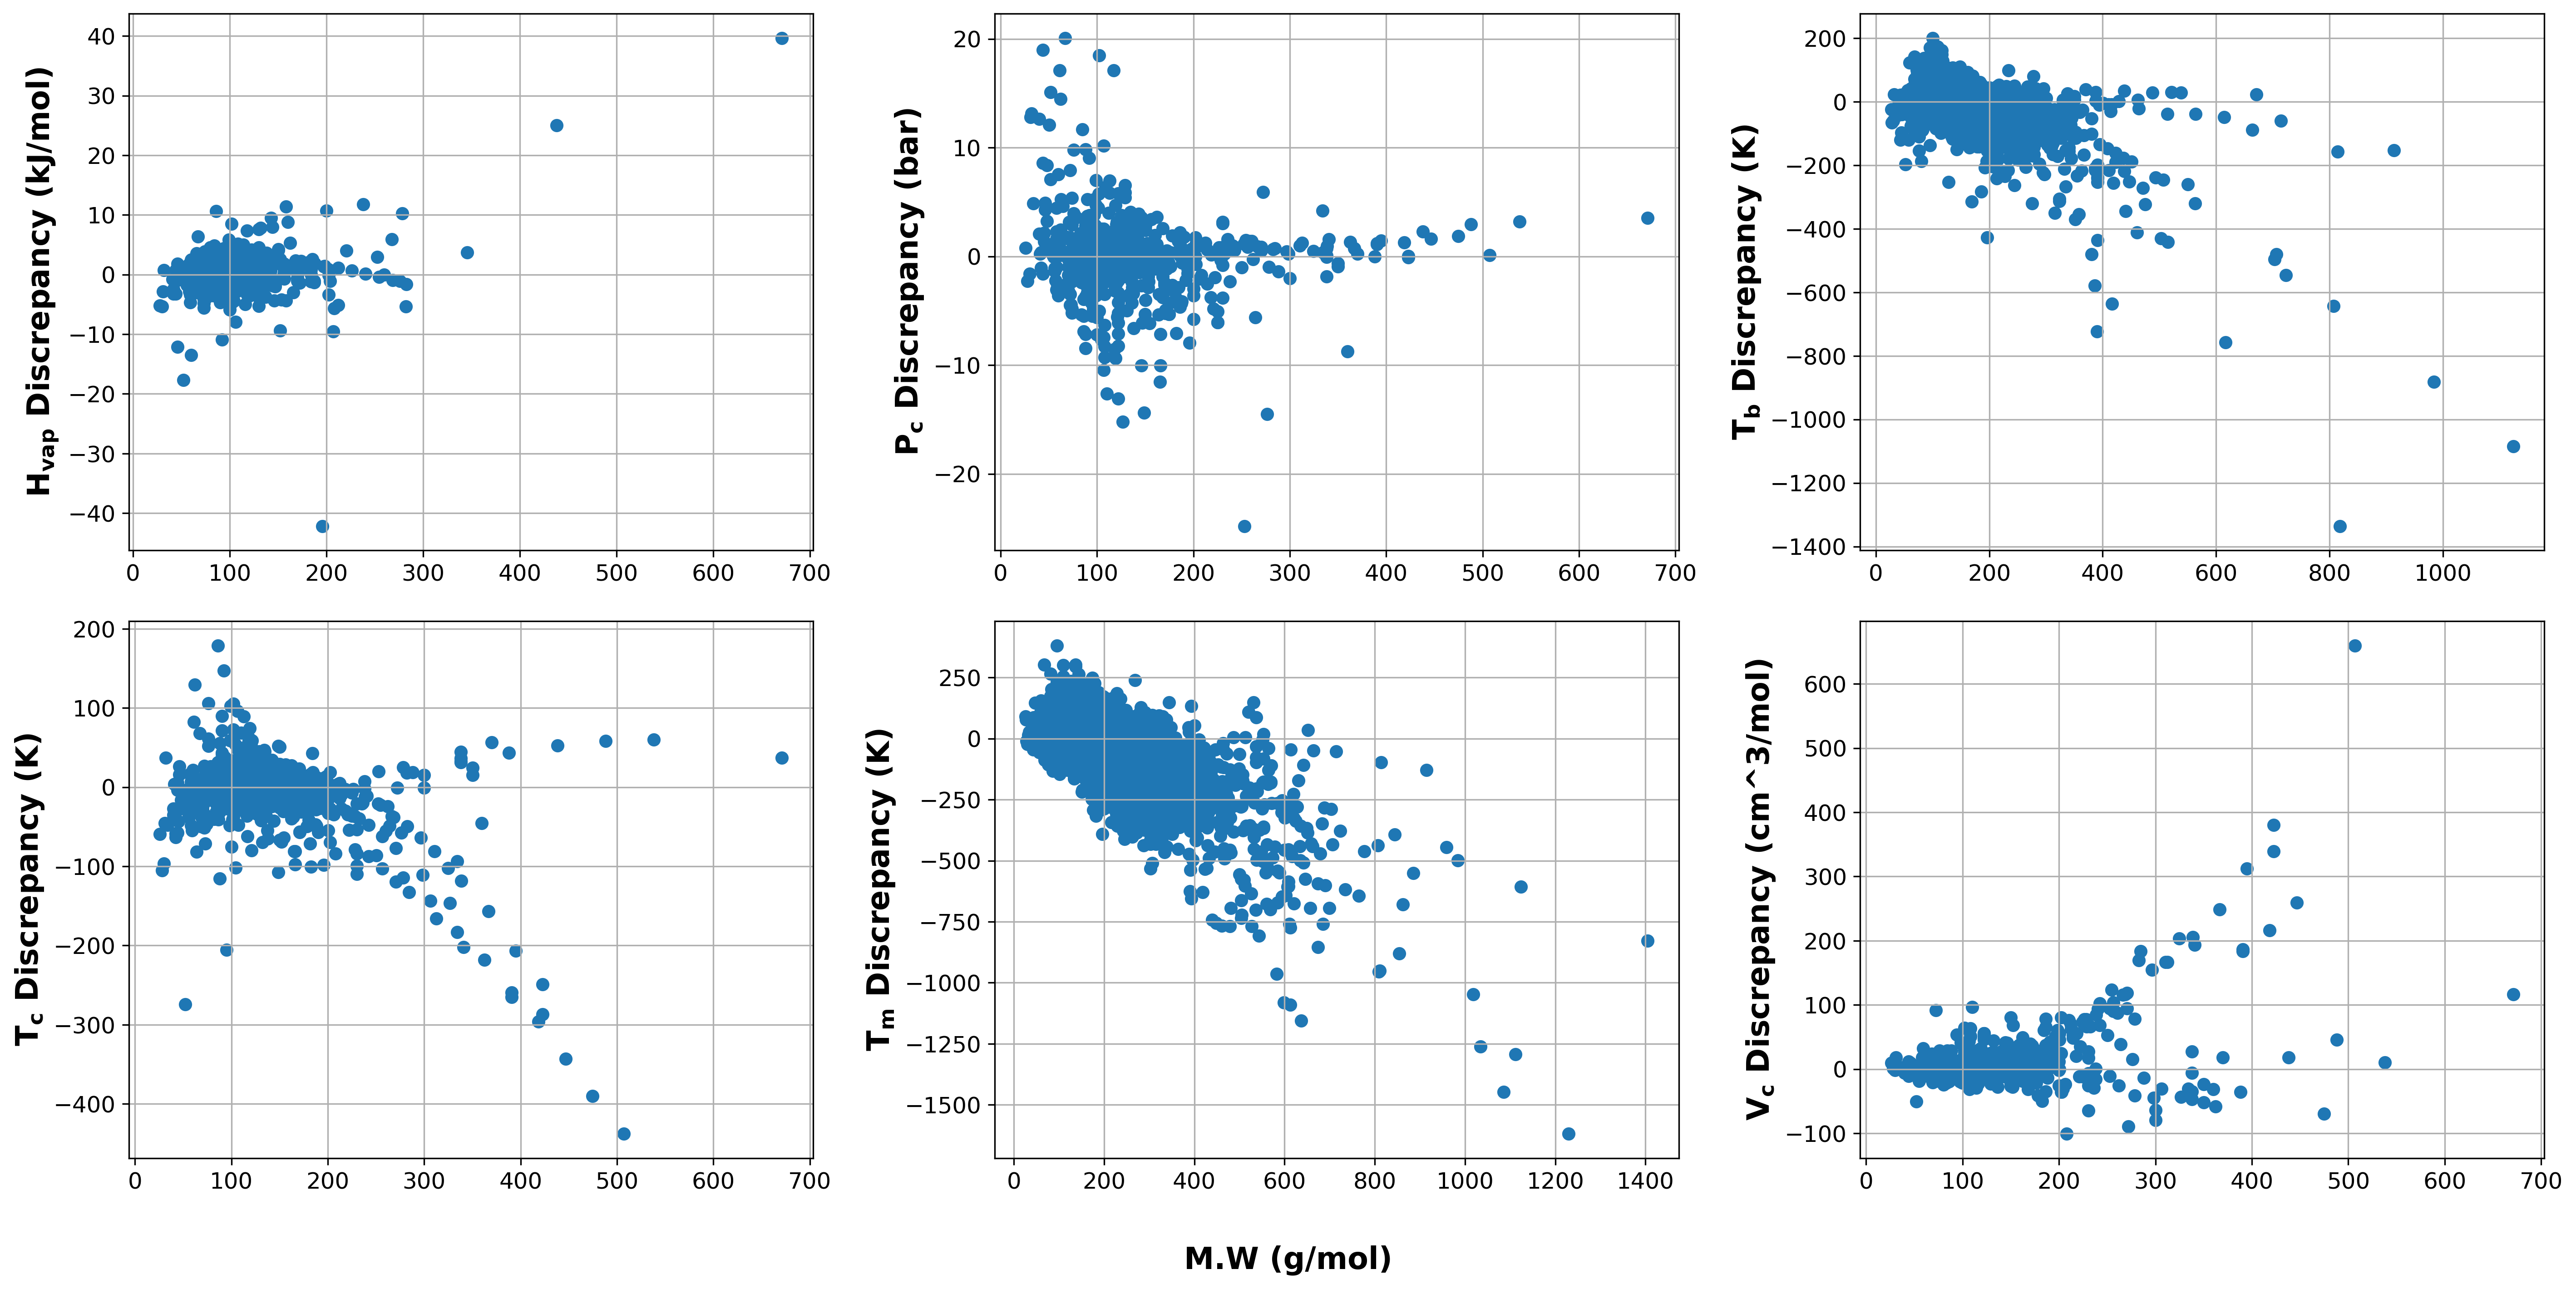
\includegraphics[width=\textwidth]{"./MW_vs_Disc.png"} %Add 6 figure 2D plots of GP Data
    \caption{Data visualization for all properties of interest. For each subplot, the x-axis is the molecular weight, the y-axis is the discrepancy between the experimental and GC predicted property value.}
    \label{fig:Data_Vis_Disc}
\end{figure}

\begin{figure}[H] %Move to SI
    \centering
    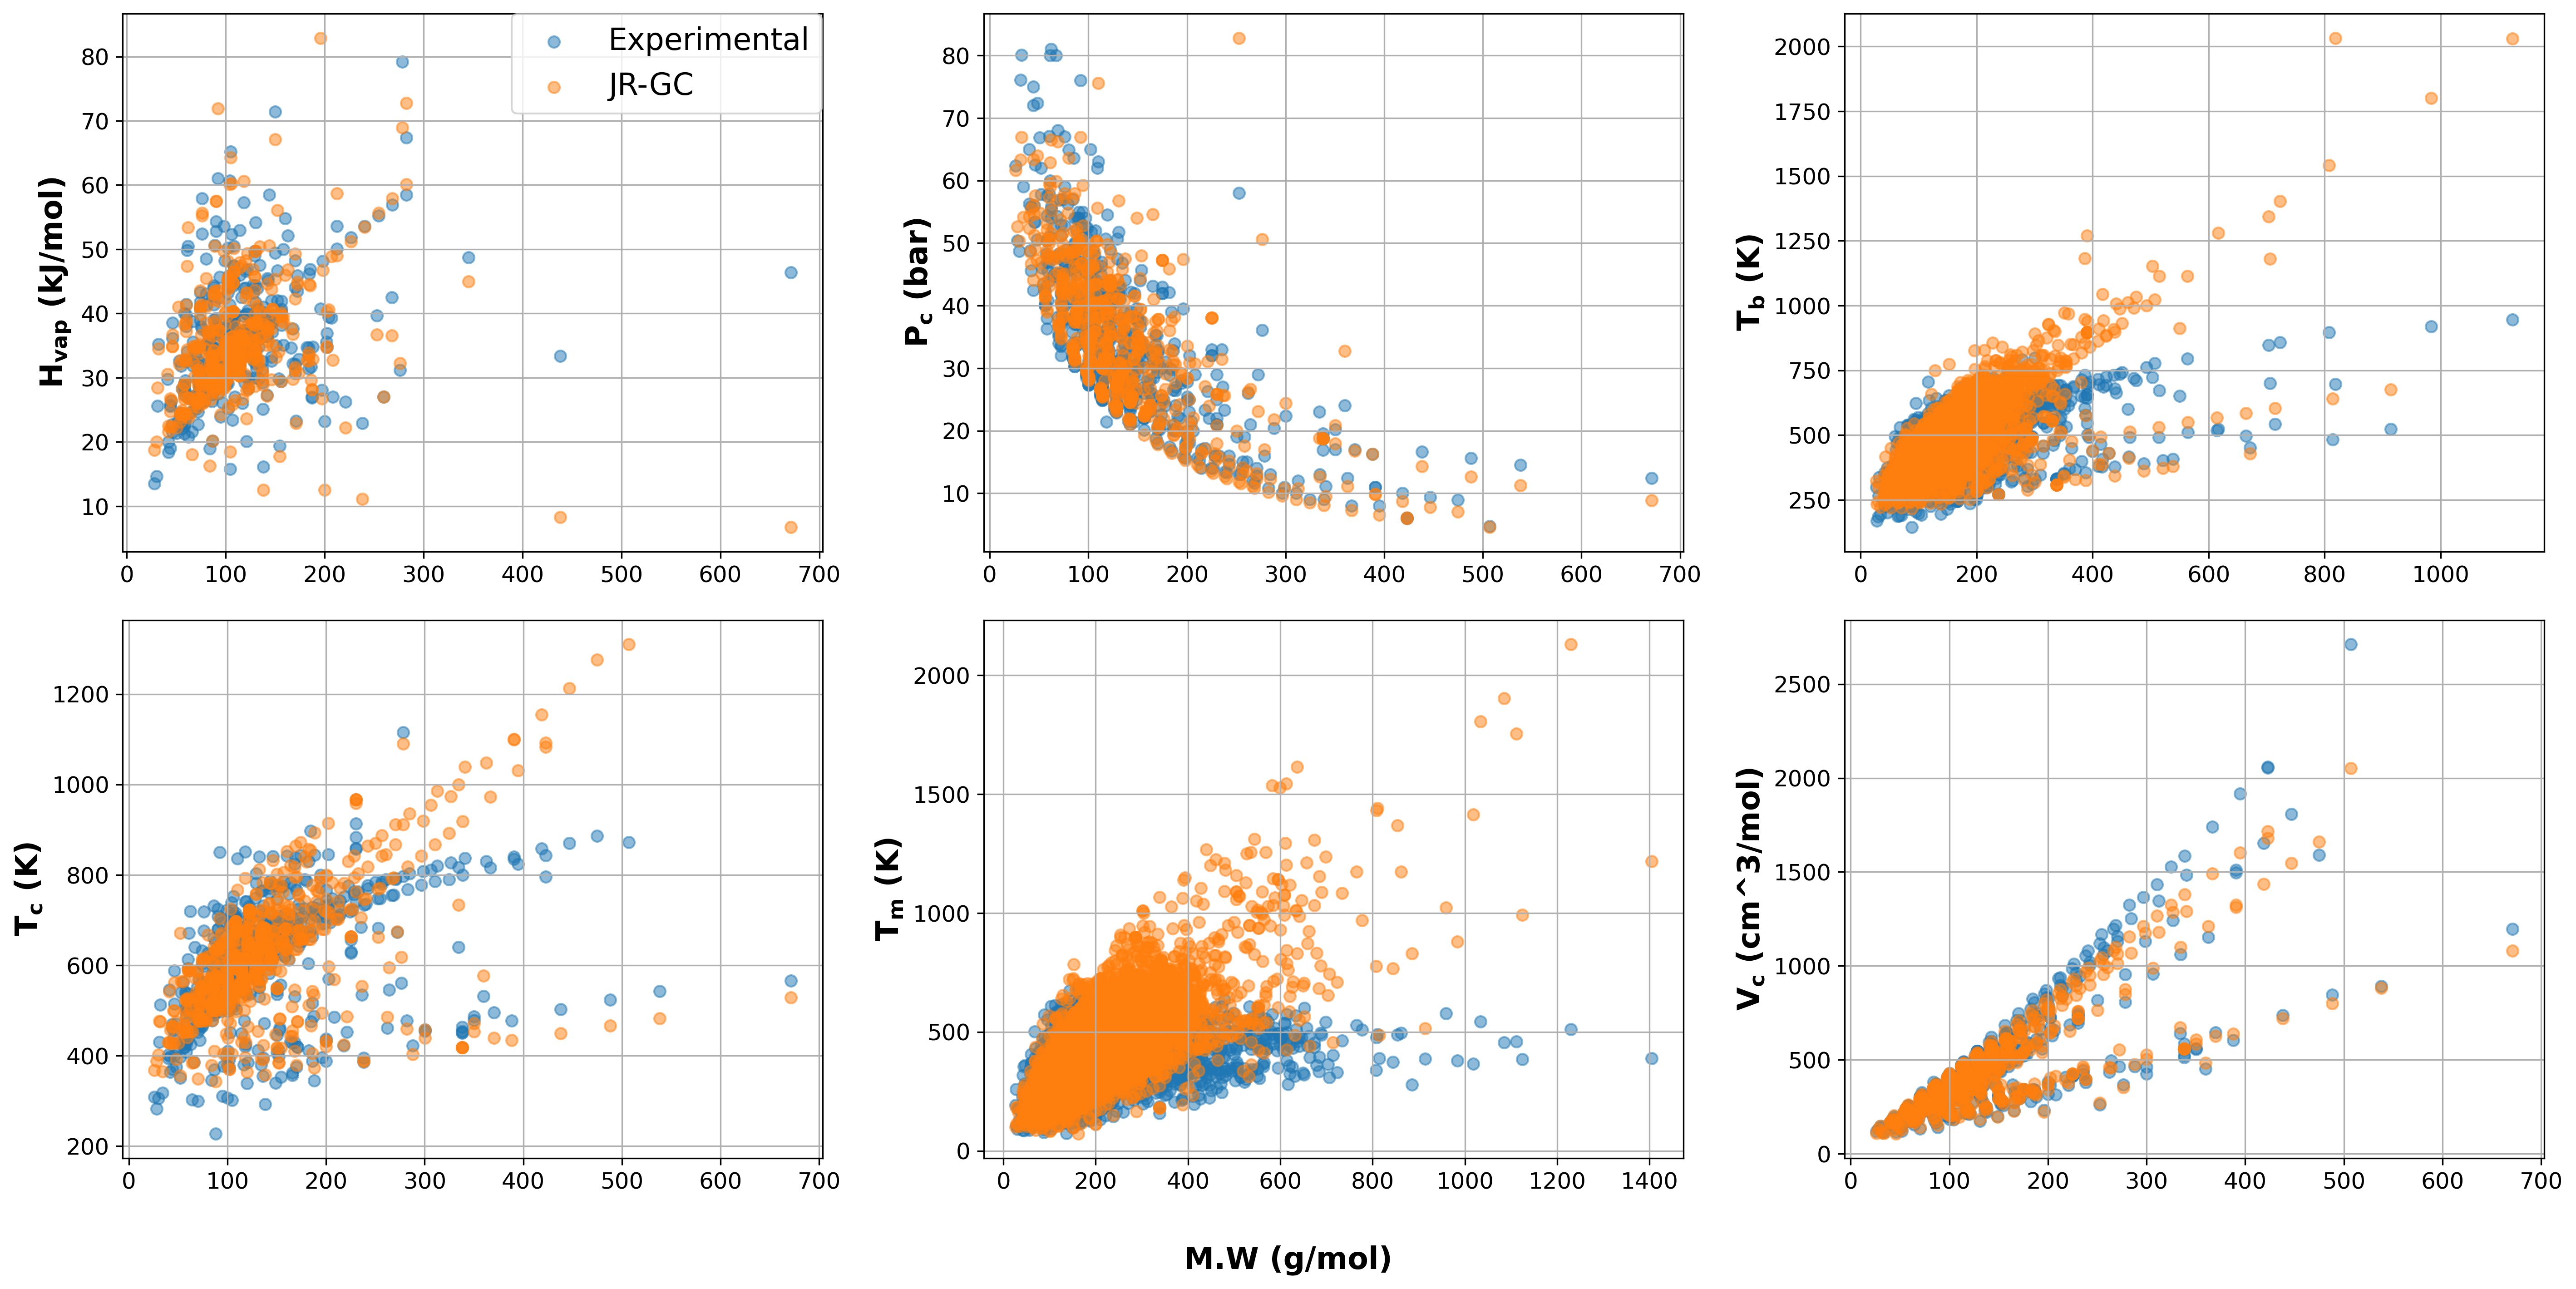
\includegraphics[width=\textwidth]{"./MW_vs_Prop.png"} %Add 6 figure 2D plots of GP Data
    \caption{Data visualization for all properties of interest. For each subplot, the x-axis is the molecular weight, the y-axis is the experimental property value (orange) or GC predicted property value (blue).}
    \label{fig:Data_Vis_Prop}
\end{figure}

\subsection{GP Modeling}

\adnote{Once the results are in place, AD will make a first pass at reconciling these two version of the GP section. The discussion in the results will drive what goes here versus in the SI.}

%Introduction to a kernel function and mean and variance predictions
\mcnote{GP Introduction. A short alternative to KJ's description below. Can be updated to match KJ notation and "GPs in the context of this work" if wanted}
To describe a Gaussian Process (GP), consider a dataset $D = \{(\xvec_i, \yexp[i]\}) \vert \xvec_i \in \mathbb{R}^d, \text{ and } \yexp[i] \in \mathbb{R}, \forall \, i \in \{1,. . ., n\}$ with inputs $\mathbf{X}$ and outputs $\yexpvec[]$. Here $\xvec$ represents the GC model predictions ($\Ygcvec$) and molecular weight ($\textbf{M.W}$) for all molecules $n$, and $\yexpvec$ represents the experimental predictions for any property \textbf{P}. If we assume that experimental data noise is independent and identically distributed with zero mean and constant variance, $\sigma_{\yexp[i]}^2$,it follows that $\yexp[i] = f(\xvec_i) + \epsilon$ where the noise is defined by $\epsilon \sim \mathcal{N}(0,\sigma_{\yexp[i]}^2)$. The GP then seeks to estimate $\yexp[i] = f(\xvec_i) + \epsilon$ as a normal distribution with mean function, $m(\xvec_i)$ for $m(\xvec_i): \mathbb{R}^d \rightarrow \mathbb{R}$, and covariance matrix, $k(\xvec_i, \xvec_i^{\prime})$ for $k: \mathbb{R}^d \times \mathbb{R}^d \rightarrow \mathbb{R}$ \cite{Frazier2018AOptimization}. We then define our GP model for all $\mathbf{X}$:
\begin{gather*}
     \yexpvec \sim \mathcal{GP} = \mathcal{N}(\boldsymbol{\mu}, \mathbf{K})
\end{gather*}

We note that this model can be classified as a hybrid model \cite{koh} since the mean function of the GP is actually a physics-based model with no stochastic component. 

\noindent where $\boldsymbol{\mu} = (m(\xvec_1), \dots, m(\xvec_n))^\intercal$ and
\begin{gather}
    \mathbf{K}= 
    \left(
    \begin{matrix}
        k(\xvec_1,\xvec_1) & \dots & k(\xvec_1,\xvec_n) \\
        \vdots & \ddots & \vdots \\
        k(\xvec_n,\xvec_1) & \dots & k(\xvec_n,\xvec_n)
    \end{matrix}\right).
\end{gather}

We note that from a purely modeling perspective, the best accuracy will be achieved by modeling each property separately with a different GP mean function and covariance matrix given the trends in the available data. However, this requires modeling expertise and given that much of the data range for each property with regards to molecular weight has already been explored, we opt to use one general model framework which is likely to capture all properties under study in this work and any future properties of interest. In the context of using JR GC predictions to train a GP model, we determined that the discrepancy of the JR GC model and experimental data is a function of molecular weight but that the relationship between the two was not always immediately obvious. However in all cases we expect that JR GC model and the experimental property data to be linearly proportional. As such, while we use both molecular weight and JR GC predictions as training data features, we implement a linear mean function which relies solely on the original JR GC predictions. We fix the hyperparameters associated with the mean function such that $\boldsymbol{\mu} = \Ygcvec$.  Other model forms which were considered can be found in SI section XX. 

The covariance matrix, often called the kernel, indicates how GP features relate to each other and the smoothness of the feature. In this work, the rational quadratic (RQ) kernel is used since it accounts for varying amounts of smoothness in each dataset through hyperparameter $\alpha$. We also add a white kernel to account for uncertainty in the experimental data. The full kernel function for any two data points is defined by \eqref{kernel_final}. Mat\`ern $\frac{1}{2}$, Mat\`ern $\frac{3}{2}$, Mat\`ern $\frac{5}{2}$, and the SE kernels are examined in section XX and are defined in SI section (reference SI section).

\begin{equation}
    k(\xvec_i,\xvec_j) = \sigma_f^2 \left(1 +\frac{1}{2 \alpha} \,\mathbf{r}^\intercal \,{\ell}^{-1} \,\mathbf{r} \right)^{-\alpha} + \sigma_w^2\delta_{i,j}
    \label{kernel_final}
\end{equation}

\noindent where  $\mathbf{r} = \xvec_i - \xvec_j$, $\sigma_f^2$ is the amplitude (variance) of the process, and $\ell$ is a length scale which controls the smoothness of the function, $\sigma_w$ is the variance of the experimental noise, applied through the Kronecker delta function $\delta_{i,j}$:
\begin{gather*}
    \delta_{i,j} = 
    \begin{cases}
        0, & i\neq j,\\
        1, & i= j.
    \end{cases}
\end{gather*}

We note that the best fitting hyperparameters $\hat{\mathbf{h}} \in [\alpha, \ell, \sigma_{f}, \sigma_{w}]$ are inferred via maximum likelihood estimation during GP training via equation \eqref{eq: lml}. This method balances maximizing model fit and minimizing model complexity. However, we note that this process should be repeated multiple times as the solution to \eqref{eq: lml} is non-convex and often has many locally optimal solutions. 
\begin{gather}
    \hat{\mathbf{h}} := \arg \min_{\mathbf{h}} \, \frac{n}{2}\log{2\pi} + \frac{1}{2}\log{|\mathbf{K}|} +  \frac{1}{2}\,(\mathbf{y}-\boldsymbol{\mu})^\intercal \, (\mathbf{K})^{-1}\,(\mathbf{y}-\boldsymbol{\mu}). \label{eq: lml}
\end{gather}

To make predictions about some new data set $\xvec^*$ using the trained GP model we note that our training and new data follow a joint multivariate normal distribution. That is,
\begin{gather*}
    \begin{bmatrix}
        \mathbf{y} \\
        \mathbf{y}_*
    \end{bmatrix}
    \sim 
    \mathcal{N}\left(
    \begin{bmatrix}
        \boldsymbol{\mu}\\
        \boldsymbol{\mu}_*
    \end{bmatrix},
    \begin{bmatrix}
        \mathbf{K}_{nn} & \mathbf{K}_{n*} \\
        \mathbf{K}_{*n} & \mathbf{K}_{**}
    \end{bmatrix} \right).
\end{gather*}

\noindent Predictions $\mathbf{y}_*$ can then be described by the conditional distribution of the new data set given the training data set.

% \begin{gather}
%     \mathbf{y}_* \,|\, \xvec, \mathbf{y} \sim \mathcal{N}(\boldsymbol{\mu}_* + \mathbf{K}_{*n}\,(\mathbf{K}_{nn})^{-1}\,(\mathbf{y}-\boldsymbol{\mu}), \mathbf{K}_{**} - \mathbf{K}_{∗n} \,(\mathbf{K}_{nn})^{-1}\,\mathbf{K}_{n*}).   
% \end{gather}

%General implementation details
GP models were implemented using GPflow \cite{Matthews2017GPflow:TensorFlow}. In this work, a white kernel is used to account for experimental noise and $\sigma_w$ is always trained starting from an initial value of 1.0. The hyperparameter tuning was implemented using scipy.optimize \cite{Virtanen2020SciPyPython} with the Limited-memory Broyden–Fletcher–Goldfarb–Shanno Bound (L-BFGS-B) algorithm to perform maximum likelihood estimation and was repeated ten times to avoid local hyperparameter solutions. On the first training pass, hyperparameters were all initialized at 1.0. On subsequent repeats, $\ell$, $\sigma^2_{rq}$, and $\alpha$ were uniformly selected from bounds $(0, 100]$, $(0, 1.0]$, and $(0, 100]$  respectively. Optimization bounds for $\ell$ and $\sigma^2_{rq}$ were set as $[10^{-5}, 10^2]$ and optimization bounds for $\alpha$ were set to $[10^{-5}, 5\times 10^3]$.

\mcnote{Commenting out condition number stuff}
% We use the condition number to determine the numerical stability of our models. The condition number is an indication of how small perturbations in the inputs can affect the outputs \cite{Foster2009}. As a rule of thumb, the number of significant digits lost in addition to those from machine precision is proportional to the logarithmic scaled value of a condition number \cite{NumMathComput}. Ideally, a condition number should be as close to one as possible and a condition number that is much greater than one (in this case we used 500 as a cutoff) is ill-conditioned. That is, a small change in the inputs has significant impact on the output.

\alltodo{Do the primary authors think the reader knows what Baysian inference is? Maybe a paragraph long section before GP basics that says what it is on a high level followed by Bayes law would be helpful for vocab like likelihood, prior, evidence, etc.}
\mcnote{The readers will not know what Bayesian inference is, but I think a whole paragraph to explain these terms might not be necessary. You've done a good job of explaining them in your sections below.}
\\
\kjnote{Begin KJ proposal for explaining GPs}
\mcnote{I have commented out KJs explanation and consolidated the GP methods to <3 pages at Barnabas's request. See above.}
\kjnote{Thanks for commenting this out as opposed to deleting. Happy to help make this shorter. When this is sent to the PI's, can you guys include what I wrote as an addendum or leave it in blue? AD can help us merge the sections. Thank you!}
\adnote{I uncommented this part from KJ so I can read and merge together.}
\subsubsection{Gaussian Process Basics}
A stochastic process is a (infinite) collection of random variables indexed by a set $\{\xvec\}$. A Gaussian process (GP) is a stochastic process where any finite number of random variables have a joint Gaussian distribution. Let $\xvec_i \in \reals^d$ denote an index and $f: \reals^d \rightarrow \reals$ denote a random variable that is indexed by $\xvec$ (i.e., the stochastic process). A GP is specified by a mean function
 \begin{gather}
     m(\xvec) := \mathbb{E}\,[f(\xvec)] \label{eq: mean}
 \end{gather}
 and a covariance function
 \begin{gather}
     k(\xvec, \xvec') := \text{Cov}\,[f(\xvec), f(\mathbf{x'})]. \label{eq: cov}
 \end{gather}
 The notation $f(\xvec)\sim \mathcal{GP}(m(\xvec), \, k(\xvec,\xvec'))$
 denotes that $f(\cdot)$ follows a GP distribution with mean function $m(\cdot)$ and covariance function $k(\cdot,\cdot)$. Equivalently, by the definition of a GP, for any finite subset $\xvec_1, \dots, \xvec_n$ of the random variables, $\mathbf{f}=(f(\xvec_1),  \dots, f(\xvec_n))^\intercal$ follows a multivariate normal distribution with a mean vector and covariance matrix governed elementwise by \eqref{eq: mean} and \eqref{eq: cov}, respectively. That is, $\mathbf{f} \sim \mathcal{N}(\boldsymbol{\mu}, \mathbf{K}),$ where $\boldsymbol{\mu} = (m(\xvec_n), \dots, m(\xvec_n))^\intercal$ and
 \begin{gather} 
     \mathbf{K} = 
     \left(
     \begin{matrix}
         k(\xvec_1,\xvec_1) & \dots & k(\xvec_1,\xvec_n) \\
         \vdots & \ddots & \vdots \\
         k(\xvec_n,\xvec_1) & \dots & k(\xvec_n,\xvec_n)
     \end{matrix}\right).
 \end{gather}

In Bayesian nonparametrics, a GP is used as a prior for a random variable indexed by an infinite set. Upon observing a finite subset of these random variables, the posterior is another GP. This is commonly applied in regression settings to recover latent functions.

\subsubsection{Model Selection and Kernels}

When deploying GPs for regression, (lack of) prior information of the latent function is encoded through the mean and covariance functions. \kjtodo{write a sentence here about the mean function} This section focuses on how to choose stationary kernel functions for modeling the covariance of the GP that are common in application literature \kjtodo{references needed}. For a more generalized perspective on classes of kernel functions, the interested reader is referred to \citeauthor{Genton} \cite{Genton}.

\adnote{Which kernel did we use for the main model? Thoughts on just keeping the main kernel here and introducing the alternate kernels in the corresponding results section? Although this is a little unorthodox, it could greatly streamline the methods.}

\kjnote{I introduced three kernels to support the model selection figure. They can be moved to wherever the primary authors think they fit best, I just need to reference them in my section.}

In mathematics, a \textit{kernel} refers to a function that defines a similarity measure between pairs of points. In the context of GPs, a kernel is a positive-definite function that defines the covariance structure. For example, the squared exponential (SE) (i.e., Gaussian) kernel is given by
\begin{gather}
     k_{\text{SE}}(\xvec_i,\xvec_j) = \sigma_f^2 \exp \left(-\frac{1}{2}\, \mathbf{r}^\intercal \,\boldsymbol{\Lambda}^{-1} \,\mathbf{r} \right), \label{eq: sekernel}
 \end{gather}
 where $\mathbf{r} = \xvec_i - \xvec_j$ is the distance between two points, $\sigma_f^2$ is the variance of the process, and $\boldsymbol{\Lambda}$ is a matrix of length scales that control the smoothness of the function. The SE kernel assumes the underlying function is infinitely differentiable. Thus, the SE kernel is widely used due to ability to model smooth functions \alltodo{advice needed: does this last sentence require a citation?}. Furthermore, a modeler can structure the length scale matrix $\boldsymbol{\Lambda}$ to encode additional smoothness assumptions of the underlying function. This is covered in detail at the end of this section. 

 A more general form of \eqref{eq: sekernel} is the rational quadratic (RQ) kernel given by
 \begin{gather}
     k_{\text{RQ}}(\xvec_i,\xvec_j) = \sigma_f^2 \left(1 +\frac{1}{2 \alpha} \,\mathbf{r}^\intercal \,\boldsymbol{\Lambda}^{-1} \,\mathbf{r} \right)^{-\alpha}. \label{eq: rationalquadkernel}
 \end{gather}
 The RQ kernel can model a wider range of functions by adjusting the parameter $\alpha$. In the limit $\alpha \rightarrow \infty$, it is approximately the SE kernel \eqref{eq: sekernel}. Thus, the RQ kernel is more flexible than the SE kernel. If the modeler wishes the function to exhibit variations at multiple length scales, the RQ kernel is more suitable than the SE kernel.

 Finally, we review the Mat\'ern kernel governed by
 \begin{gather}
     k_{\text{Mat\'ern}}(\xvec_i,\xvec_j) = \sigma_f^2 \,\frac{2^{1-\nu}}{\Gamma(\nu)} \, \left(\sqrt{2\nu} \, \mathbf{r}^\intercal \,\boldsymbol{\Lambda}^{-1} \,\mathbf{r} \right)^{\nu}\, K_\nu  \left(\sqrt{2\nu} \, \mathbf{r}^\intercal \,\boldsymbol{\Lambda}^{-1} \,\mathbf{r} \right). \label{eq: maternkern}
 \end{gather}
 Here, $\nu$ is a smoothness parameter, $\Gamma(\cdot)$ is the Gamma function, and $K_\nu(\cdot)$ is the modified Bessel function of the second kind. Like the RQ kernel \eqref{eq: rationalquadkernel}, Matérn kernels are a generalization of the SE kernel. It can be shown that in the limit $\nu \rightarrow \infty$, the Mat\'ern kernel becomes the SE kernel. Moreover, the SE kernel assumes infinitely differentiable (smooth) functions, while the Matérn kernel allows for varying degrees of smoothness through $\nu$. These kernels can be useful when modeling real-world phenomena with unknown or varying smoothness, thereby providing more flexibility. Common choices for $\nu$ in machine learning and GP regresison applications literature include 3/2 and 5/2 \alltodo{GP modeling authors: please include the citations here that motivated the decision to include these kernels}. 

 In principled inference, the structure of of the length scale matrix $\boldsymbol{\Lambda}$ is used to model (lack of) prior information about the function. In an isotropic GP, a single length scale is used for all input dimensions. Mathematically, this means the length scale matrix is written as $\boldsymbol{\Lambda} = \lambda^2 \, \mathbf{I}$. This modeling choice enforces that all input dimensions are equally important and have the same effect on the output. Alternatively, if one wanted to use separate length scales for each input dimension, one could elect kernels \eqref{eq: sekernel} - \eqref{eq: maternkern} with automatic relevance detection. This allows the kernel to capture the varying relevance of different dimensions, meaning some dimensions can be more influential than others in predicting the output. Mathematically, this means the length scale matrix is written as $\boldsymbol{\Lambda} = \text{diag}(\lambda_1^2,\dots,\lambda_d^2)$.

 \subsubsection{Gaussian Processes for Regression}
 Consider the regression setting in which a modeler is supplied with a dataset $\mathcal{D} = \{(\xvec_i, y_i)\}_{i=1}^n$ composed of $n$ pairs of regressors $\xvec_i \in \reals^d$ and observations $y_i \in \reals$. The objective is to recover the latent data generating process $f(\cdot)$. In most practical settings, the underlying process is perturbed by noise $\varepsilon$. That is,
 \begin{gather*}
     y_i = f(\xvec_i) + \varepsilon_i, \quad i \in \{1,\dots, n\},
 \end{gather*}
 where $\varepsilon_i \stackrel{\text{i.i.d.}}{\sim} \mathcal{N}(0,\sigma_n^2)$. In GP regression (GPR) \alltodo{remove this acronym if not used later on in the text}, it is assumed that $f(\cdot)\sim \mathcal{GP}(m(\cdot),k(\cdot,\cdot))$. This assumption is called the prior. By linearity of expectation,
 \begin{gather*}
     \mathbb{E}\,[y_i\,|\,\xvec_i] = m(\xvec_i)
 \end{gather*}
 and
 \begin{gather*}
     \text{Cov}\,[y_i\, | \,\xvec_i, y_j \, | \,\xvec_j] = k(\xvec_i, \xvec_j) + \sigma_n^2 \,h_{i,j},
 \end{gather*}
 where $h_{i,j}$ is the Kronecker delta function
 \begin{gather*}
     h_{i,j} = 
     \begin{cases}
         0, & i\neq j,\\
         1, & i= j.
     \end{cases}
 \end{gather*}
 The goal in the regression setting is to predict $f(\cdot)$ over a test set $\xmatrix_*$. By the GP prior on $f(\cdot)$, the finite set of training and test outputs follow a joint multivariate normal distribution. That is,
 \begin{gather*}
     \begin{bmatrix}
         \mathbf{y} \\
         \mathbf{f}_*
     \end{bmatrix}
     \sim 
     \mathcal{N}\left(
     \begin{bmatrix}
         \boldsymbol{\mu}\\
         \boldsymbol{\mu}_*
     \end{bmatrix},
     \begin{bmatrix}
         \mathbf{K} +\sigma_n^2\,\mathbf{I} & \mathbf{K}_* \\
         \mathbf{K}^\intercal_* & \mathbf{K}_{**}
     \end{bmatrix} \right).
 \end{gather*}
 Here, $\mathbf{K}_*$ is the $n \times |\text{test}|$ covariance matrix and $\mathbf{K}_{**}$ is the $|\text{test}| \times |\text{test}|$ covariance matrix. 
 To make predictions at the test points $\xmatrix_{*}$, one can leverage the conditional distribution of the test outputs given the training data $\mathcal{D}$. This is done with the finite-dimensional conditional distribution
 \begin{gather}
     \mathbf{f}_* \,|\, \xmatrix_*, \mathcal{D} \sim \mathcal{N}(\mathbf{K}_{*}^\intercal \,(\mathbf{K} +\sigma_n^2 \mathbf{I})^{-1}\,(\mathbf{y}-\boldsymbol{\mu}),  \mathbf{K}_{**} - \mathbf{K}_{*}^\intercal \,(\mathbf{K}+\sigma_n^2\,\mathbf{I})^{-1}\,\mathbf{K}_{*}).   \label{eq: gppredict}
 \end{gather}
 Note that this is the predictive distribution for $\mathbf{f}_*$. The predictive distribution for $\mathbf{y}_*$ can be obtained by adding $\sigma_n^2\, \mathbf{I}$ to the covariance in \eqref{eq: gppredict}.

 \subsubsection{Hyperparameter Estimation and Criteria for Model Selection}
 As shown in the \alltodo{Model Selection and Kernels section, rename if you change this name}, the behavior of mean and kernel functions are somewhat dictated by their parameters $\boldsymbol{\theta} = (\sigma_n, \sigma_f, \lambda_1,\dots,\lambda_d)^\intercal$. If the elements of $\boldsymbol{\theta}$ are not chosen by the practitioner, they must be inferred from the sample data $\mathcal{D}$. Furthermore, one might be interested in comparing the performance of several GP models and selecting the best performing model. The evidence (i.e., marginal likelihood) accomplishes both objectives.

 The evidence is given by
 \begin{gather*}
     p(\mathbf{y}\, | \, \xmatrix) = \int p(\mathbf{y}\, | \, \mathbf{f}) \,  p(\mathbf{f}\, | \, \xmatrix) \, \text{d}\mathbf{f},
 \end{gather*}
 where we marginalize over the the function values $\mathbf{f}$. Given that both $p(\mathbf{y}\, | \, \mathbf{f})$ and $ p(\mathbf{f}\, | \, \mathbf{X})$ are Gaussian, the marginal likelihood can be computed in closed form. Moreover, the marginal likelihood has distribution
 \begin{gather*}
     \mathbf{y}\, | \, \mathbf{X} \sim \mathcal{N}(\boldsymbol{\mu}, \mathbf{K} + \sigma_n^2 \,\mathbf{I}),
 \end{gather*}
 and the expression for the evidence is the p.d.f. of this distribution
 \begin{gather*}
     p(\mathbf{y}\, | \, \mathbf{X}) = (2\pi)^{-n/2}\,\vert \mathbf{K} + \sigma_n^2 \,\mathbf{I}\vert^{-1/2}\,\exp \left( -\frac{1}{2}\,(\mathbf{y}-\boldsymbol{\mu})^\intercal \, (\mathbf{K} + \sigma_n^2 \,\mathbf{I})^{-1}\,(\mathbf{y}-\boldsymbol{\mu})\right),
 \end{gather*}
 where $|\cdot|$ is the determinant. In practice, the negative log evidence is minimized to find the optimal $\hat{\boldsymbol{\theta}}$, that is
 \begin{gather}
     \hat{\boldsymbol{\theta}} := \arg \min_{\boldsymbol{\theta}} \, \frac{n}{2}\log{2\pi} + \frac{1}{2}\log{|\mathbf{K} + \sigma_n^2 \,\mathbf{I}|} +  \frac{1}{2}\,(\mathbf{y}-\boldsymbol{\mu})^\intercal \, (\mathbf{K} + \sigma_n^2 \,\mathbf{I})^{-1}\,(\mathbf{y}-\boldsymbol{\mu}). \label{eq: lml}
 \end{gather}
 The terms in \eqref{eq: lml} aid in model selection as follows. The first component is the normalization constant, the second component is the model complexity penalty, and the third component is the model first to the data. A smaller model fit term indicates better model fit. The determinant of the covariance matrix reflects the area or volume of the function space covered by the model \kjtodo{make sure its both area and volume}. Thus, the larger (smaller) the determinant, the greater (lesser) the complexity of the model. Thus, \eqref{eq: lml} balances the tradeoff between minimizing complexity and maximizing model fit.
 \kjnote{end of proposed text on GP modeling}


 \subsubsection{Hybrid Modeling}
 \alltodo{Feel free to move this section wherever it fits best}
 \kjnote{begin text from KJ}\\
 In their seminal work, statisticians \citeauthor{koh} \cite{koh} developed a framework for Bayesian calibration of computer models, which has become commonplace in the physical sciences. \kjtodo{write review about this}\\

 Given $n$ observations $\mathbf{y}=(y_1,\dots,y_n)^\intercal$ generated by manipulating a controlled variable $\xvec_i = (x_{i,1},\dots,x_{i,d})^\intercal$, the goal of model calibration is to find the underlying mapping $\zeta: \mathbb{R}^d \rightarrow \mathbb{R}$ that describes the physical scenario. This relationship is written as
 \begin{gather}
     y_i = \zeta(\mathbf{x}_i) + \varepsilon_i, \quad i \in \{1,\dots,n\}. \label{eq: trueprocess}
 \end{gather}

 In practice, $\zeta(\cdot)$ is unknown, and the modeler must rely on a simulation or lower-fidelity model denoted $\eta(\mathbf{x}, \boldsymbol{\theta})$. The model has parameters $\boldsymbol{\theta}=(\theta_1,\dots,\theta_p)^\intercal$ that need to be estimated from data. To account for discrepancy in the model $\eta(\cdot,\cdot)$, a model discrepancy function $\delta: \mathbb{R}^d \rightarrow \mathbb{R}$ is included. This leads to:
 \begin{gather}
      y_i = \zeta(\mathbf{x}_i) + \varepsilon_i = \eta(\mathbf{x}_i,\boldsymbol{\theta}) + \delta(\mathbf{x}_i) + \varepsilon_i, \quad i \in \{1,\dots,n\}.
 \end{gather}

 Typically, $\delta(\cdot)$ is modeled using a Gaussian Process (GP), although any nonparametric method can be used in practice. If $\eta(\cdot,\cdot)$ is computationally expensive, it can also be represented as a GP. In this work, it is assumed that $\eta(\cdot,\cdot)$ can be modeled directly and $\delta(\cdot)\sim \mathcal{GP}(m(\cdot),k(\cdot,\cdot))$. Thus, the hybrid model reduces to the GP
 \begin{gather}
     \zeta(\mathbf{x}) \sim \mathcal{GP}(\eta(\mathbf{x},\boldsymbol{\theta}) + m(\mathbf{x}), k(\mathbf{x}, \mathbf{x}'))
 \end{gather}
In this application, there are no physically-meaningful parameters $\boldsymbol{\theta}$ to estimate in the low-fidelity model. Moreover, estimation of $\zeta(\cdot)$ is accomplished by estimating the parameters in the GP mean and covariance functions.
\kjnote{end text from KJ}





\subsubsection{GPs in the context of this work}

\adnote{EM really liked this section as it helped solidify the abstract ideas in the context of the paper goal.}

In this work, we define $\mathcal{D} = \{(\Ygc[i], \text{M.W}_i), \yexp[i])\}_{i=1}^n$ for all molecules $n$ and any property of interest $y \in [H_{vap}, P_c, T_c, T_b ,T_M, V_c]$. We define $\Ygc[i] \text{ } \forall \text{ } i\in n$ as JR GC model predictions, $\text{M.W}_i \text{ } \forall \text{ } i\in n$ as the molecular weights, and $\yexp[i] \text{ } \forall \text{ } i\in n$ as the experimental values. We begin by noting that from a modeling perspective, the best accuracy will be achieved by analyzing trends in the available data and setting the GP mean and covariance functions to capture those trends. However, this requires modeling expertise and given that much of the data range for each property with regards to molecular weight has already been explored, we opt to use one general model framework which is likely to capture all properties under study in this work and any future properties of interest. The effect of model form on our results is examined in section \ref{sec:kern_sweep}.

We determined in section XX that the discrepancy of the JR GC model for each property of interest and experimental property data is a function of molecular weight but that the relationship between the two was not always immediately obvious. However in all cases we expect that JR GC model and the experimental property data to be linearly proportional. As such, while we use both molecular weight and JR GC predictions as training data features, we implement a linear mean function which relies solely on the original JR GC predictions. We fix the hyperparameters associated with the mean function such that $m(\xvec) = \Ygcvec$ where $\Ygc[i] \text{ } \forall \text{ } i\in n$ are the JR GC model predictions for $n$ molecules and any property of interest $y$. This mean function is especially appropriate when the JR GC models faithfully represent the trend of experimental data. Other model forms which were considered can be found in SI section XX. We choose the rational quadratic (RQ) kernel as the base kernel function for the GP models of every property to account for varying levels of smoothness. We add a white kernel with variance $\sigma_w$ to the RQ kernel to account for uncertainty in the experimental data such that the final covariance function used in this work is defined by \eqref{kernel_final}. 

 \begin{equation}
     k(\xvec_i,\xvec_j) = \sigma_f^2 \left(1 +\frac{1}{2 \alpha} \,\mathbf{r}^\intercal \,\boldsymbol{\Lambda}^{-1} \,\mathbf{r} \right)^{-\alpha} + \sigma_w^2\delta_{i,j} 
     \label{kernel_final}
 \end{equation} 

 GP models were implemented using GPflow \cite{Matthews2017GPflow:TensorFlow} (version \adnote{fill in}). The hyperparameter tuning was implemented using scipy.optimize \cite{Virtanen2020SciPyPython} (version: \adnote{fill in}) with the Limited-memory Broyden–Fletcher–Goldfarb–Shanno Bound (L-BFGS-B) algorithm to perform maximum likelihood estimation and was repeated ten times to avoid local hyperparameter solutions. On the first training pass, hyperparameters were all initialized at 1.0. On subsequent repeats, $\ell$ and $\alpha$ were uniformly selected from bounds $(0, 100]$ and $(0, 100]$ respectively. $\sigma^2_f$ was selected from a log-normal distribution with bounds $[0,1.0]$ and $\sigma_w$ was always initialized at $1.0$. A more nuanced method would be to initialize $\sigma_w$ as the scaled experimental uncertainty when available. Optimization bounds for $\alpha$ were set to $[10^{-5}, 10^2]$ and all other hyperparameters were optimized within bounds $[10^{-5}, 5\times 10^3]$.

 We use the condition number to determine the numerical stability of our models. The condition number is an indication of how small perturbations in the inputs can affect the outputs \cite{Foster2009}. As a rule of thumb, the number of significant digits lost in addition to those from machine precision is proportional to the logarithmic scaled value of a condition number \cite{NumMathComput}. Ideally, a condition number should be as close to one as possible and a condition number that is much greater than one (in this case we used 500 as a cutoff) is ill-conditioned. That is, a small change in the inputs has significant impact on the output.



%Stratified sampling (Dinis)
\subsubsection{Stratified sampling}
When splitting data into training and testing sets, an 80/20 split was used, and all features and labels were standardized to have zero mean and unit variance using the sci-kit-learn StandardScaler \cite{scikit-learn}. Feature-based stratified sampling was used to split the data.

\subsection{Error Metrics}
We use mean absolute error (MAE), mean absolute percent error (MAPE), coefficient of determination ($R^2$), and root mean squared error (RMSE) to quantify and critically analyze the error of our GP models. This section gives an overview of the definition of these error metrics. Note that in \eqref{eq:COD}, $\overline{y_{\text{exp}}}$ is the average value of $\mathbf{y}_{\text{exp}}$. 

\begin{equation}
    \text{MAE} = \frac{1}{N} \sum_{i=1}^{N} \left| y_{\text{exp}_i} - \mu(\mathbf{x}_i) \right|
    \label{eq:MAE}
\end{equation}

% \begin{equation}
%     \alltodo{\text{MAPE}} = \frac{1}{N} \sum_{i=1}^{N} \left| \frac{y_{\text{exp}_i} - \mu(\mathbf{x}_i)}{y_{\text{exp}_i}} \right|
%     \label{eq:MAPE}
% \end{equation}

\begin{equation}
    \text{MAPE} = \frac{1}{N} \sum_{i=1}^{N} \left| \frac{y_{\text{exp}_i} - \mu(\mathbf{x}_i)}{y_{\text{exp}_i}} \right| \times 100\%
    \label{eq:MAPD}
\end{equation}

\begin{equation}
    R^2 = 1 - \frac{\sum_{i=1}^{N} \left( y_{\text{exp}_i} - \mu(\mathbf{x}_i) \right)^2}{\sum_{i=1}^{N} \left( y_{\text{exp}_i} - \overline{y_{\text{exp}}} \right)^2}
    \label{eq:COD}
\end{equation}

\begin{equation}
    \text{RMSE} = \sqrt{\frac{1}{N} \sum_{i=1}^{N} \left( y_{\text{exp}_i} - \mu(\mathbf{x}_i) \right)^2}
    \label{eq:RMSE}
\end{equation}

\section{Results and Discussion}

\subsection{JR GC method has systematic bias and limited accuracy}

\adnote{Move Figures \ref{fig:2D_JRGC_bias} and \ref{fig:JRGC_Hvap_bias_molecules} into the introduction. This will help setup the main goal of the paper and reduce some redundancy.}

Figure \ref{fig:2D_JRGC_bias} shows the systematic bias of the JR GC predictions when compared against experimental data. Deviations from the experimental data are most pronounced for $T_m$ and $T_b$, especially at higher molecular weights. Similar but less pronounced systematic deviation of JR GC predictions from experimental data is observed for $T_c$ and $V_c$.   

\begin{figure}[H]
    \centering
    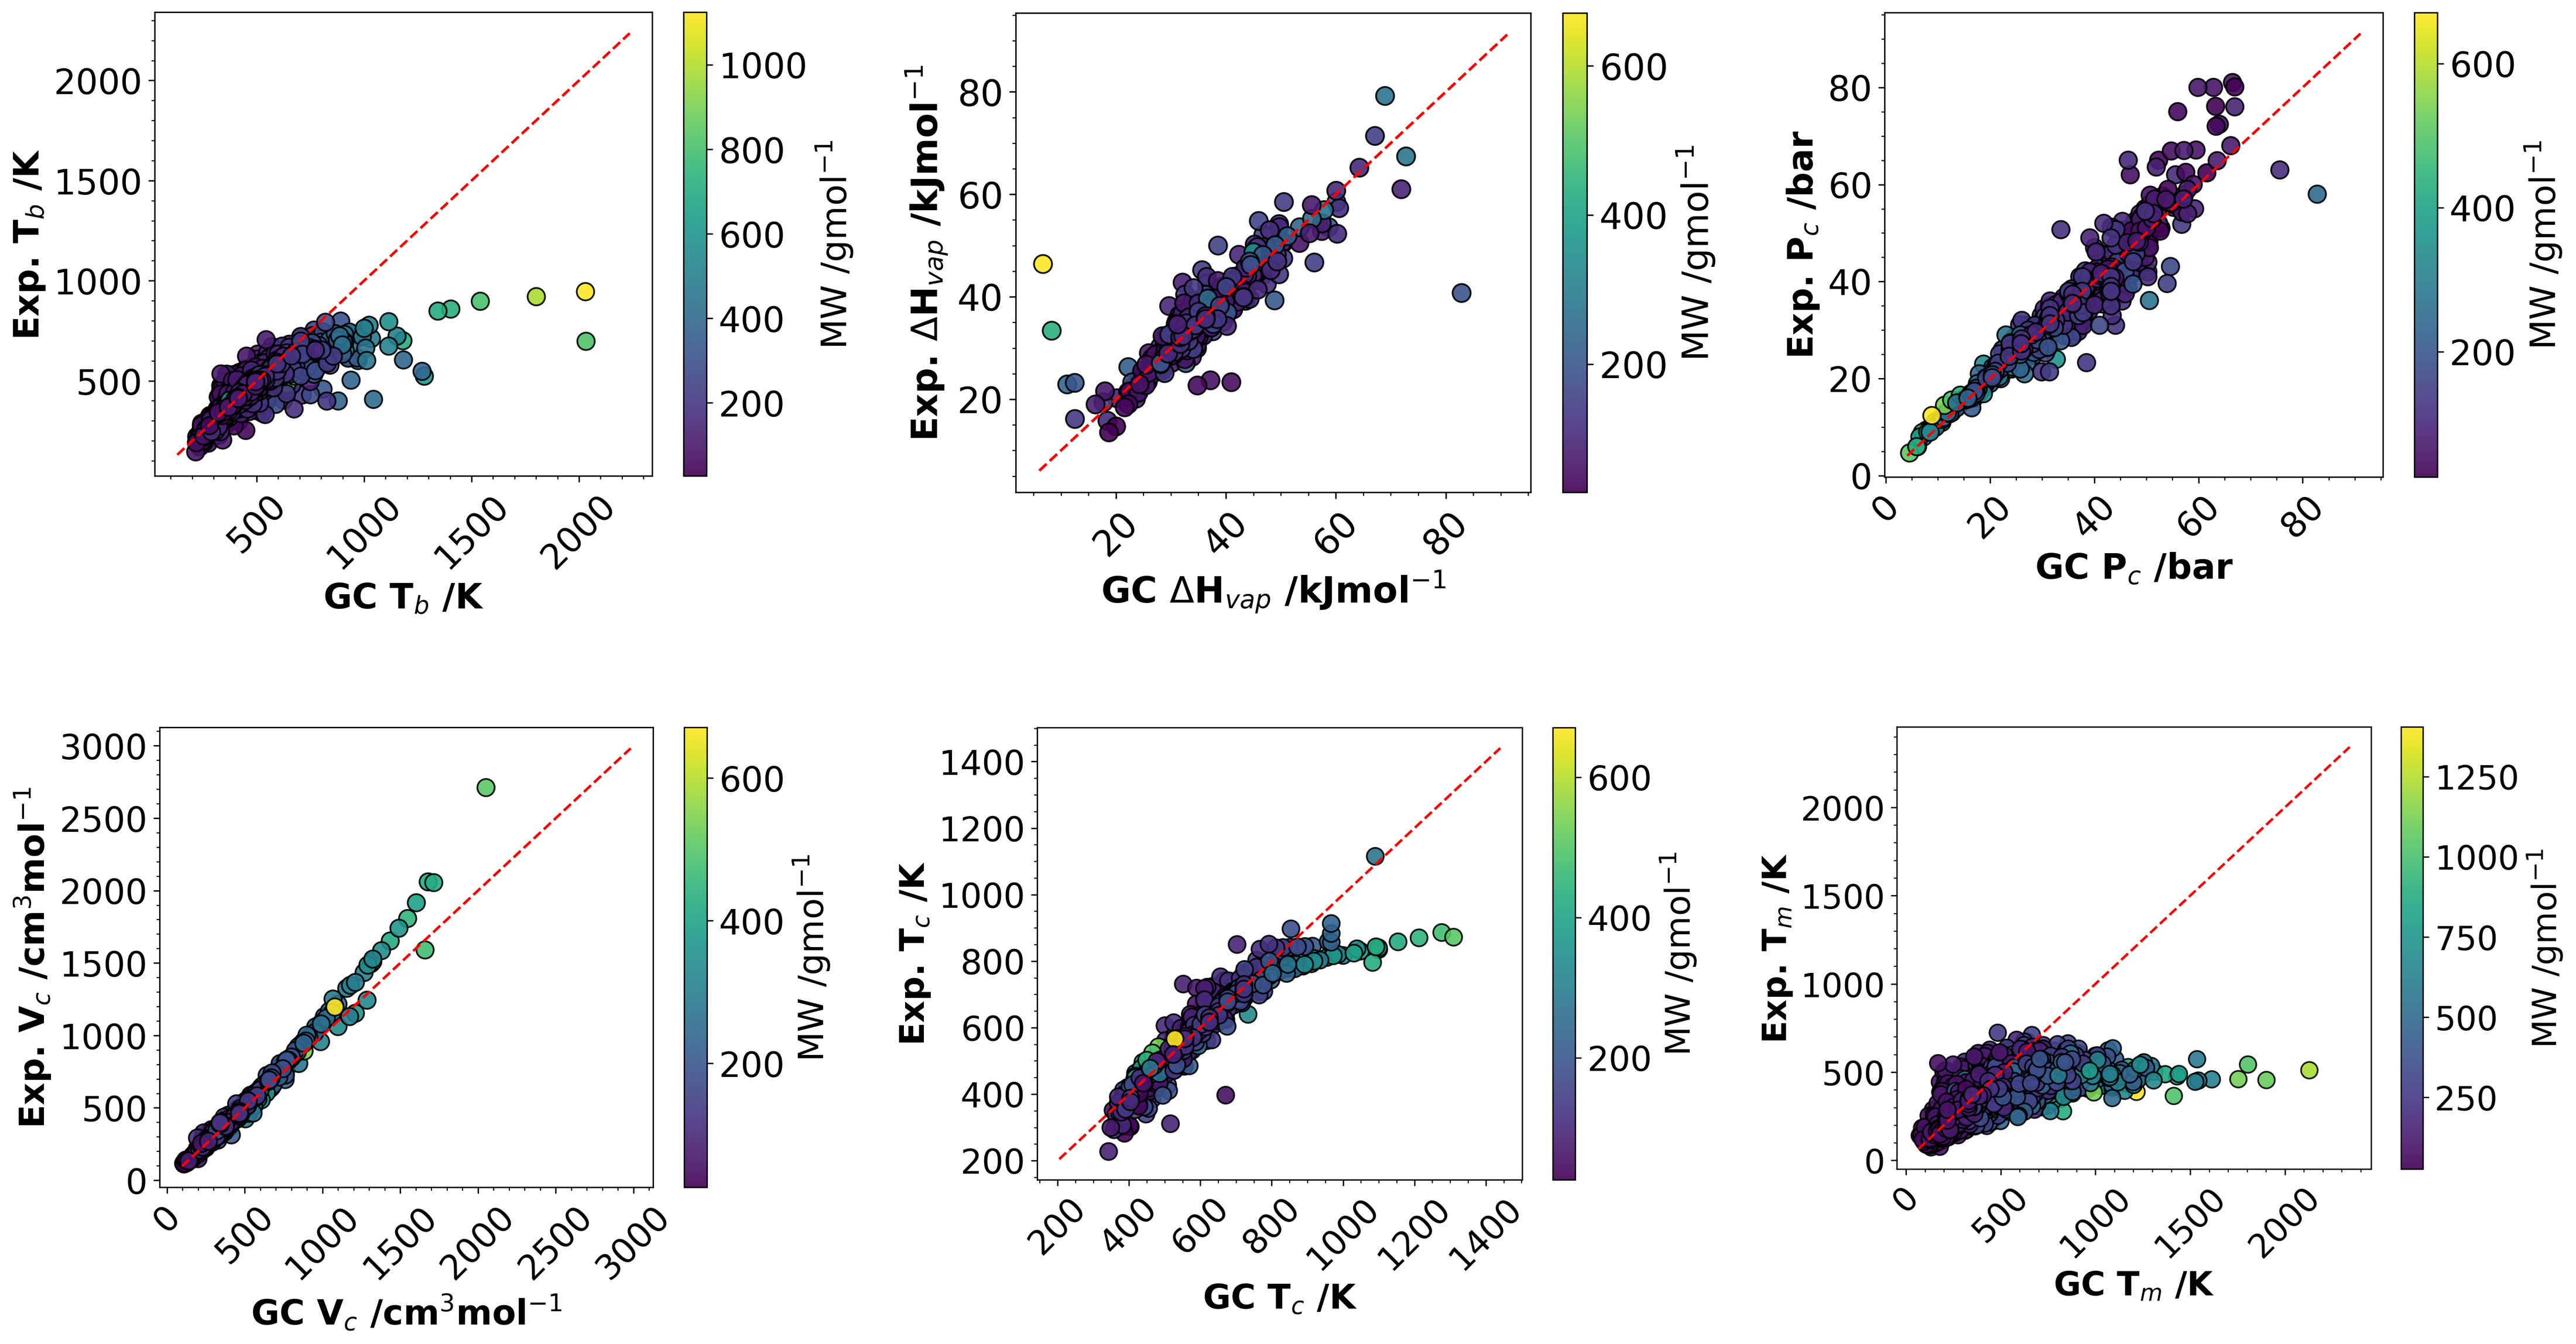
\includegraphics[width=1.1\linewidth]{images/2D_GC_bias.png}
    \caption{Parity plot of experimental data against JR GC predictions.}
    \label{fig:2D_JRGC_bias}
\end{figure}

This systematic bias is due to one of the flaws of the JR GC method, which assumes that structural units contribute to the value of these properties in a monotonous manner. Thus, we observe, for example, that the JR GC method predicts that several organic molecules would have $T_m$ values greater than 1500 $K$, which is not the case in nature. Molecules do not monotonously and boundlessly melt at higher temperatures as the structural units are added.
The systematic bias of the JR GC predictions for $\Delta H_{vap}$ and $P_c$ is more nuanced. Unlike the other properties for which the JR GC method shows systematic bias that is generally correlated with molecular weight, the systematic bias of the JR GC method for $\Delta H_{vap}$ and $P_c$ is for specific classes of molecules.
We found from our outlier detection analysis, presented in detail in the SI, that the JR GC method shows significant systematic bias in it's $\Delta H_{vap}$ predictions for highly fluorinated and highly nitrated molecules. In Figure \ref{fig:2D_JRGC_bias}, there are two points with conspicuously low JR GC $\Delta H_{vap}$ predictions. 

\adnote{Likely move Figure \ref{fig:JRGC_Hvap_bias_molecules} to the SI.}

\begin{figure}[H]
    \centering
    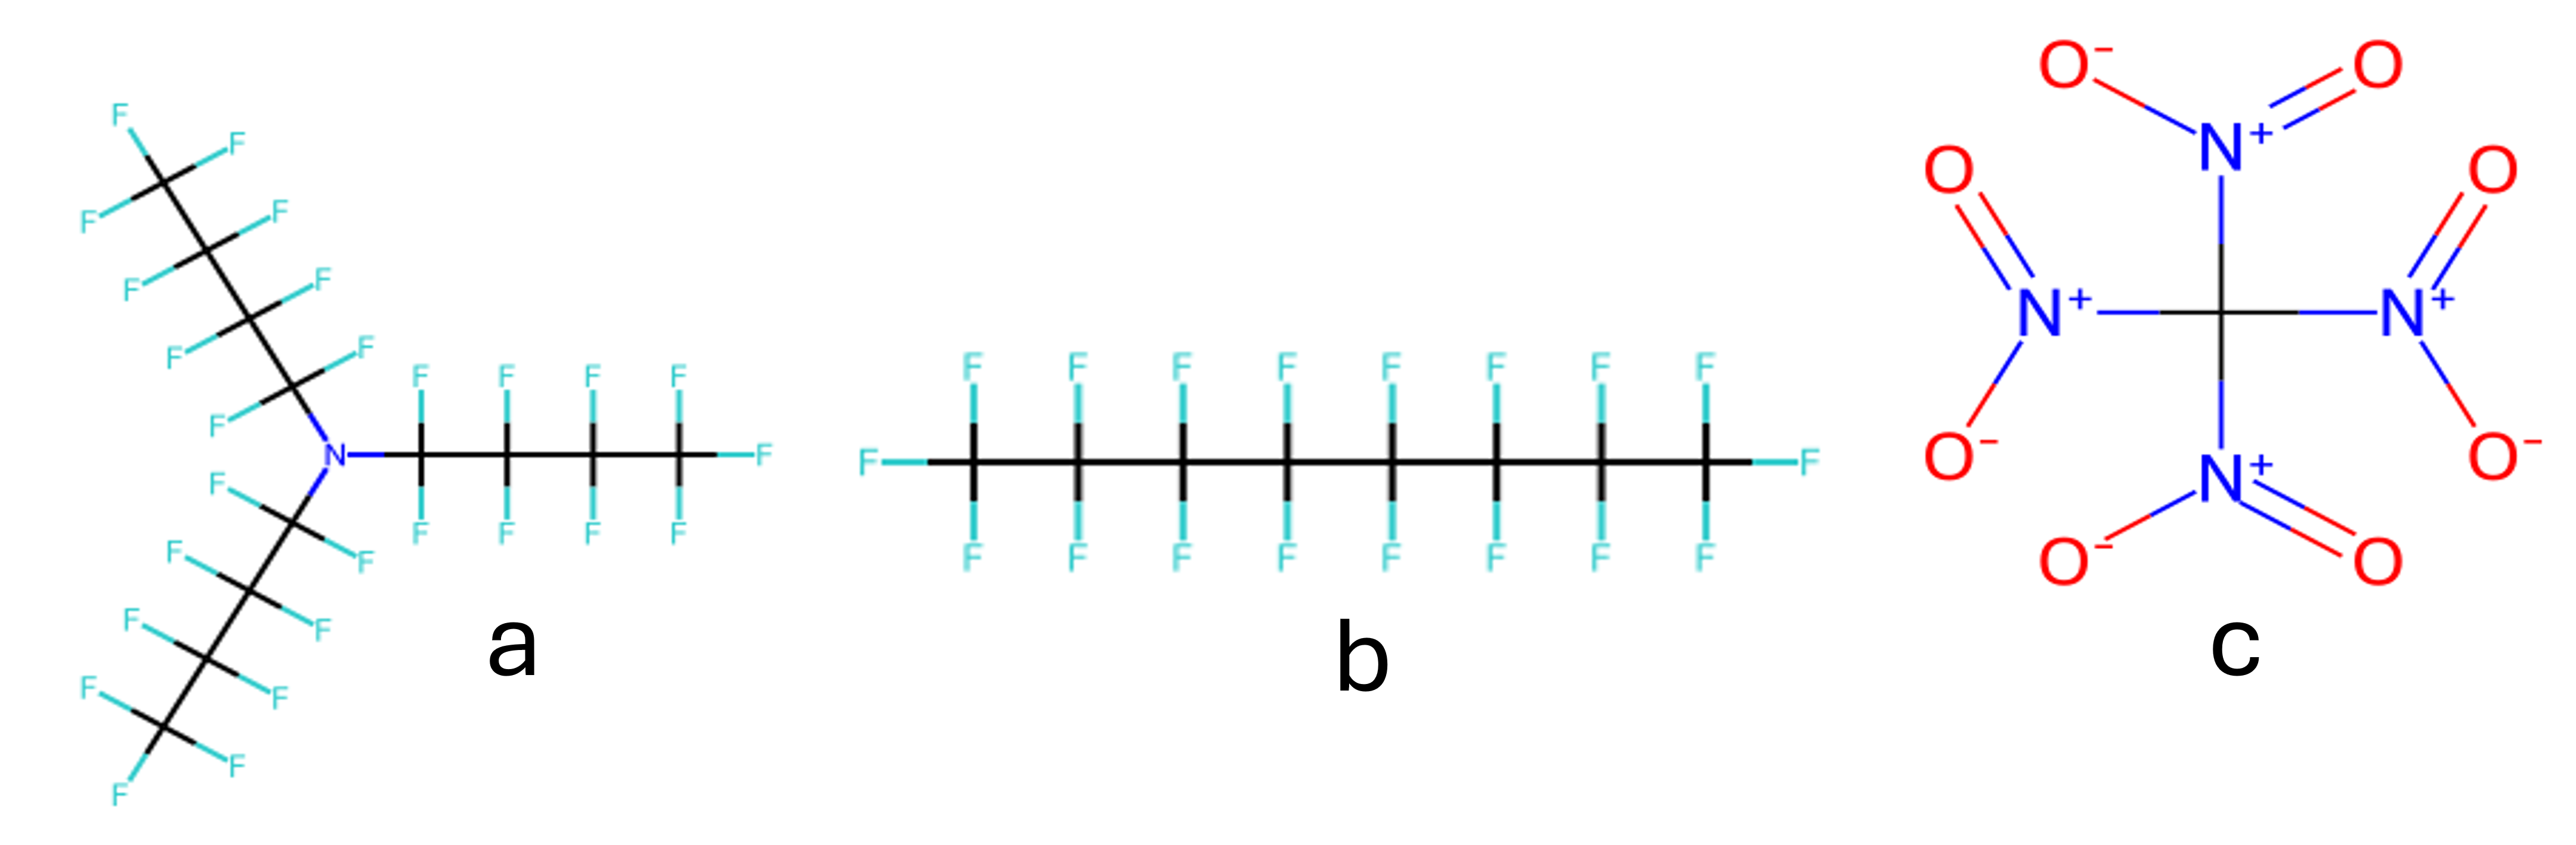
\includegraphics[width=0.8\linewidth]{images/Hvap_molecules_with_large_bias.png}
    \caption{Molecules with large bias in JR GC $\Delta H_{vap}$ predictions}
    \label{fig:JRGC_Hvap_bias_molecules}
\end{figure}

These two points correspond to molecules with moderate to high MW. The two molecules with this large underestimation in  $\Delta H_{vap}$ using the JR GC method are shown in Figure \ref{fig:JRGC_Hvap_bias_molecules} a and b. They are both highly fluorinated molecules. The group contribution of the fluorine group to $\Delta H_{vap}$ according to the JR GC method is -0.67 $kJ/mol$. This explains why, for highly fluorinated molecules, the JR GC method predicts very low values of $\Delta H_{vap}$ contrary to experimental or true values. The JR GC method could predict negative $\Delta H_{vap}$ values for sufficiently fluorinated molecules, which would be unphysical. Figure \ref{fig:JRGC_Hvap_bias_molecules} c shows another class of molecules for which the JR GC method has a large systematic bias in its $\Delta H_{vap}$ predictions. They are highly nitrated compounds like tetranitromethane shown in Figure \ref{fig:JRGC_Hvap_bias_molecules} c. The JR GC $\Delta H_{vap}$ predictions for tetranitromethane is 82.89 $kJ/mol$ and can be observed in Figure \ref{fig:2D_JRGC_bias} as the highest JR GC $\Delta H_{vap}$ prediction in our data. The JR GC method predicts that every $-NO_2$ structural unit in a molecule should contribute 16.738 $kJ/mol$ to the $\Delta H_{vap}$ of the molecule. This contribution is high and much higher than those of most other structural units in the JR GC method parameter set for $\Delta H_{vap}$. This leads to an overestimation in $\Delta H_{vap}$ for highly nitrated molecules.
A similar scenario is observed for JR GC $P_c$ predictions for highly brominated molecules.  


\begin{figure}[H]
    \centering
    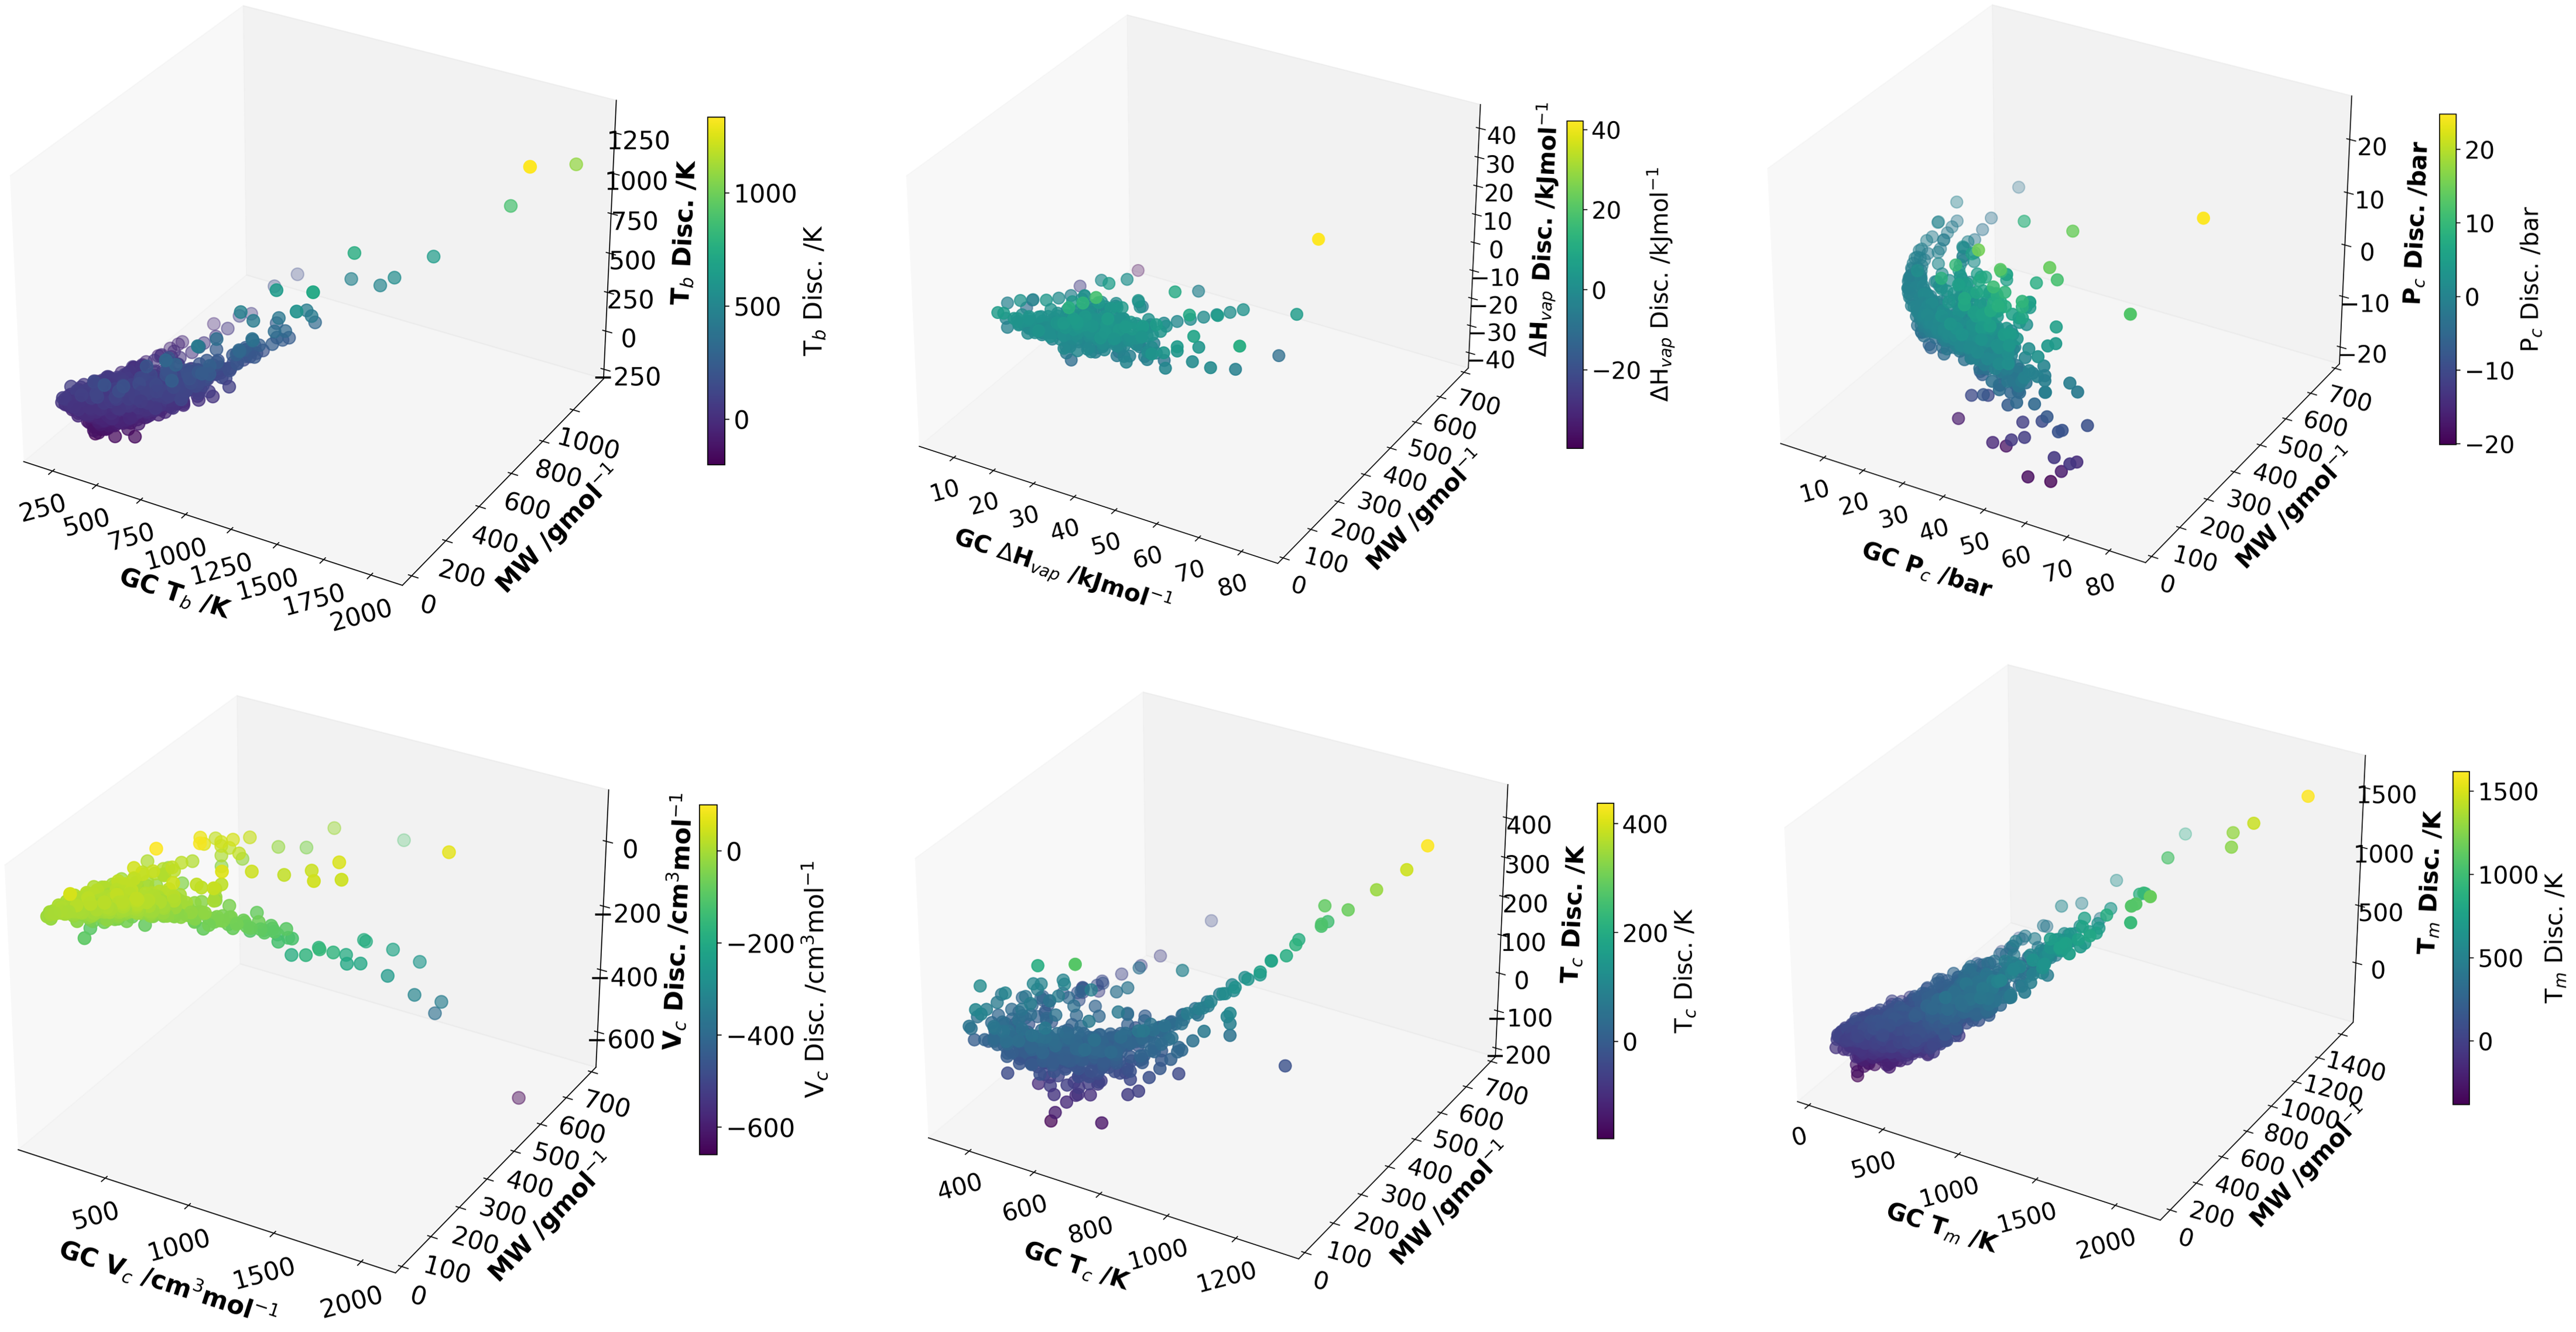
\includegraphics[width=1.1\linewidth]{images/3D_gc_mw_exp.png}
    \caption{3D surface plot of MW, JR GC predictions, and discrepancy of JR GC predictions from experimental data.}
    \label{fig:3D_JRGC_MW_disc}
\end{figure}

\adnote{This idea goes into the introduction.} Figure \ref{fig:3D_JRGC_MW_disc} shows the surfaces that we learn using a GP for each property. It also further helps to visualize the systematic bias of the JR GC method and how this bias is correlated with MW. We observe a strong correlation between the JR GC predictions discrepancy and MW for $T_m$, $T_b$, $T_c$, and $V_c$. The surfaces in Figure \ref{fig:3D_JRGC_MW_disc} generally possess a navigable structure rather than random collections of points in 3D space. This provides additional justification for why GPs are suitable for learning these surfaces.


\subsection{GCGP method accurately predicts properties and corrects systematic bias}

In this work, we used a GP to correct the systematic bias of the JR GC method. The results are presented in Figure \ref{fig:GCGP_final_results}. Figure XX in the SI show these results only for GP predicted values with 95 \% confidence interval error bars. Table XX in the SI shows the final values of the optimized GP hyperparameters for each property.
Applying the GCGP method almost doubled (0.44 to 0.86) the coefficient of determination ($R^2$) between predictions and experimental values of the testing set for $T_b$. The MAE reduced from 28.8 $K$ for the JR GC predictions to 19.5 $K$ for the GCGP predictions. 
Similarly, we also observed correction of systematic bias and significant improvement in predictive accuracy for $T_c$ as shown in Figure \ref{fig:GCGP_final_results}.

\adnote{Refactor Figure \ref{fig:GCGP_final_results} into a full-page figure with 6 rows (properties) and two columns (GC versus GCGP). EM and AD are concerned the 'black blob' hides the main point.}

\begin{figure}[H]
    \centering
    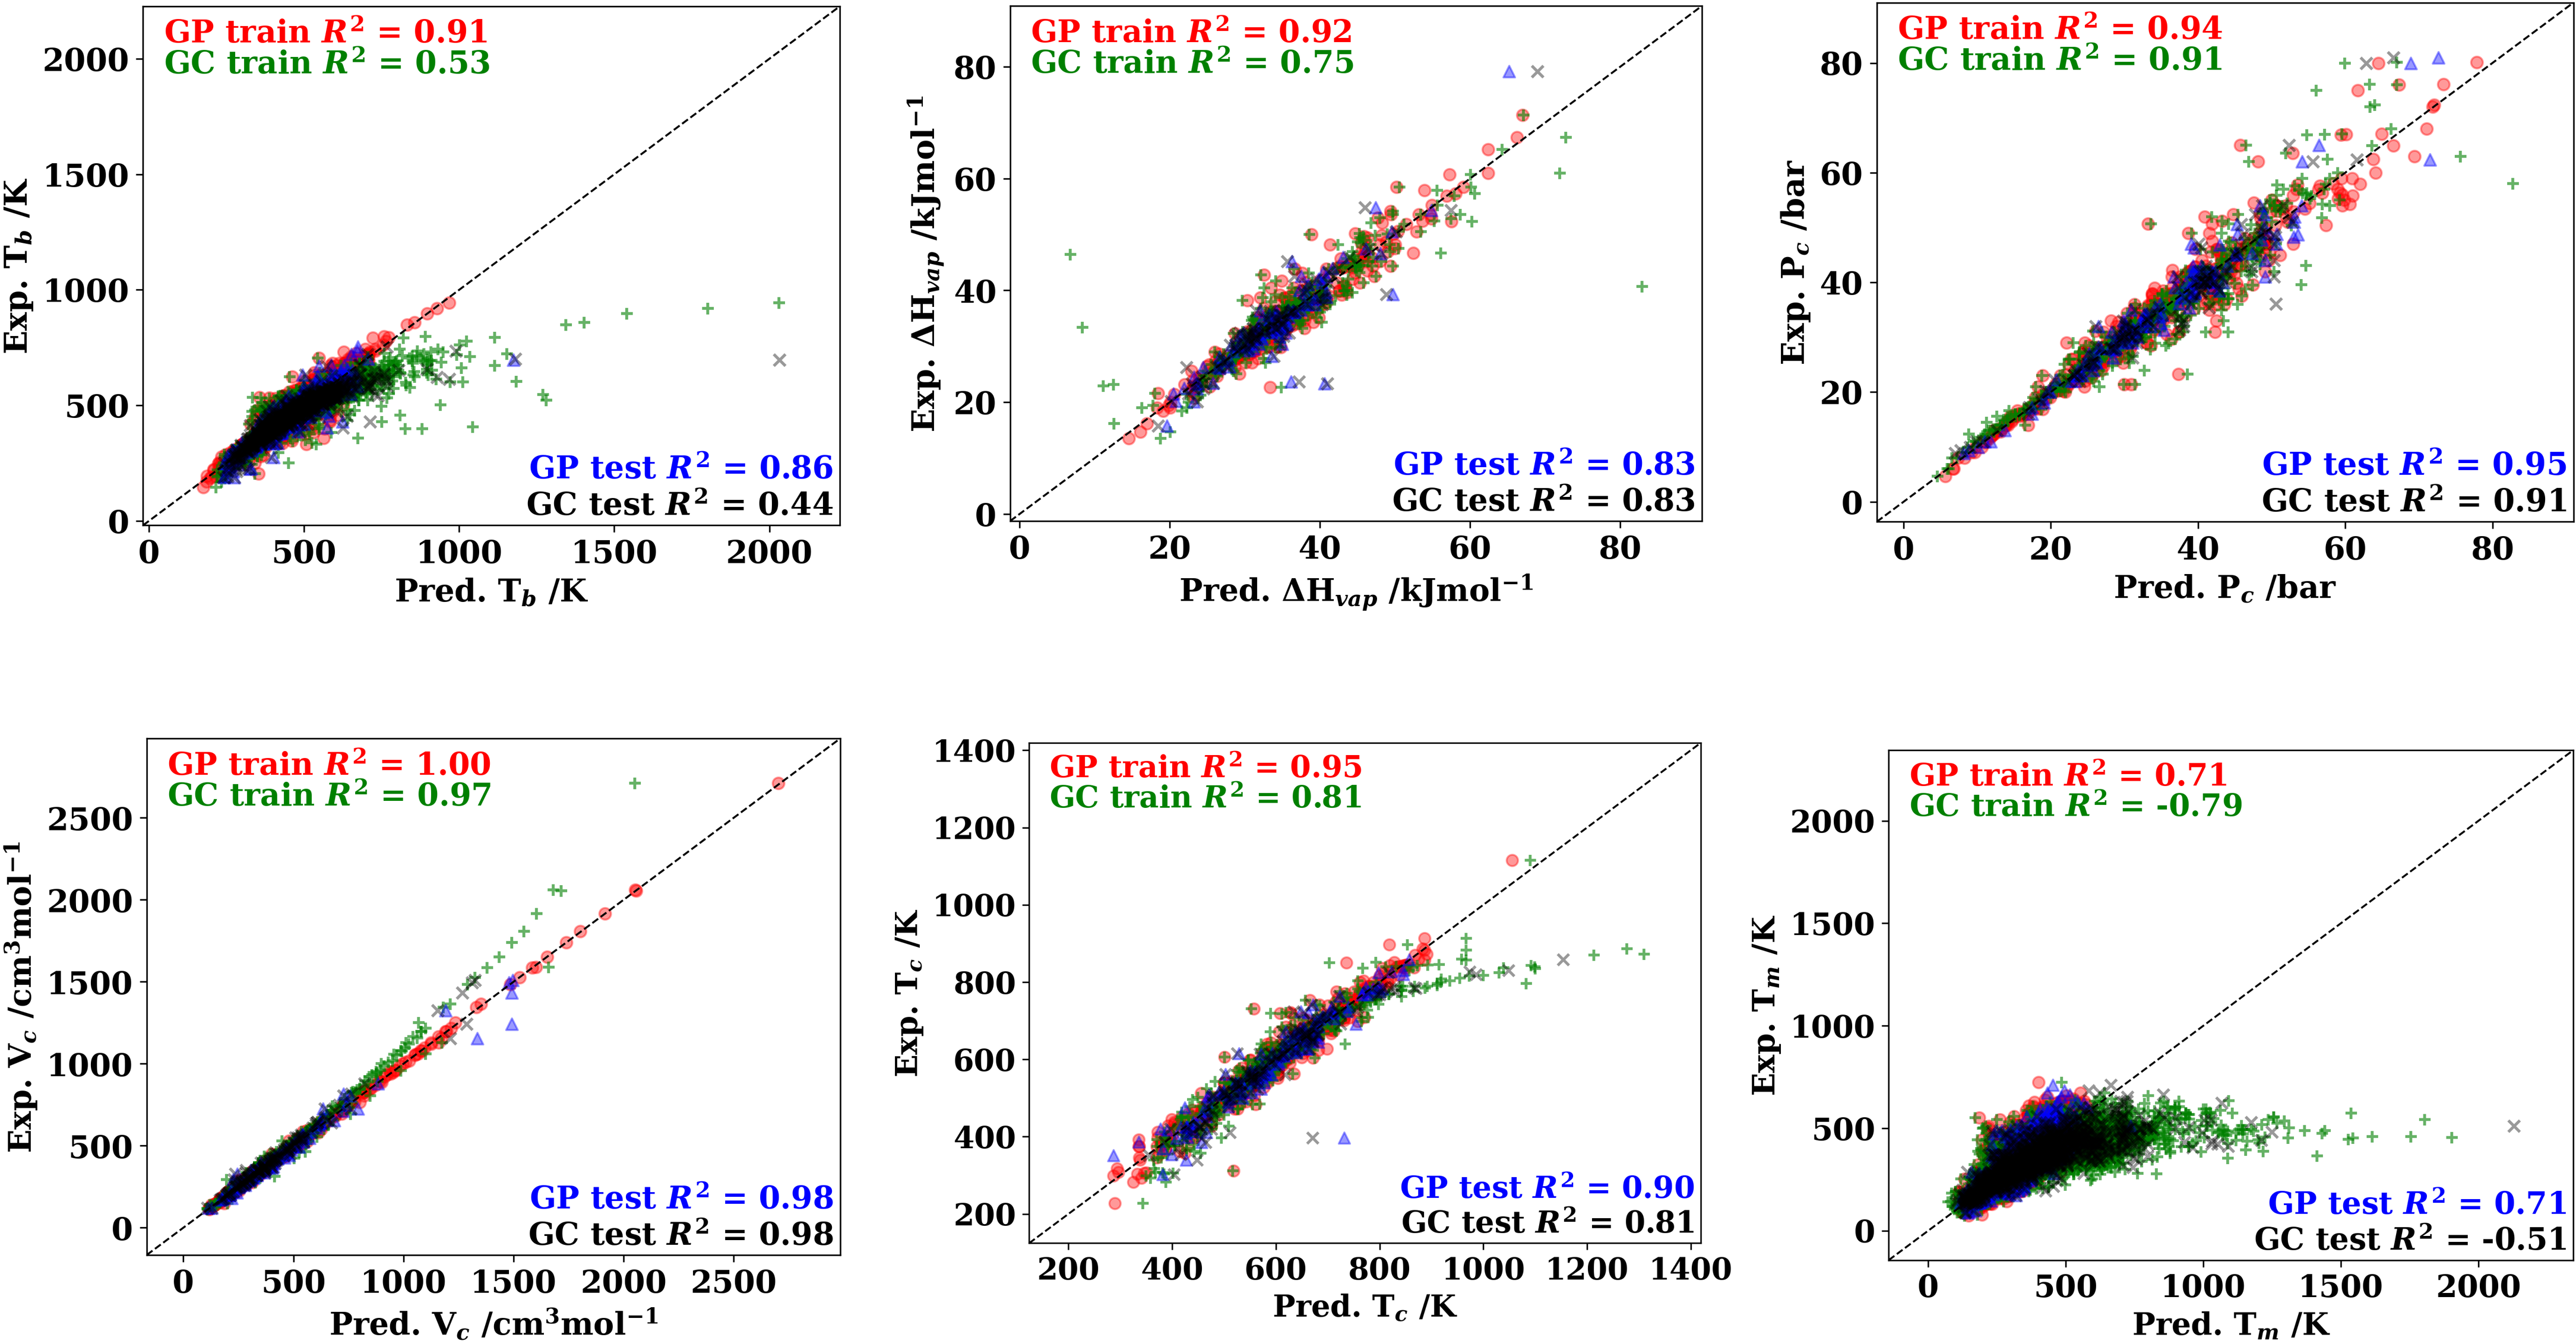
\includegraphics[width=1.1\linewidth]{images/GCGP_final_results.png}
    \caption{GCGP corrections of systematic bias in JR GC model}
    \label{fig:GCGP_final_results}
\end{figure}

 
The largest correction in systematic bias was observed for the property for which the JR GC method had the highest systematic bias - $T_m$. The testing set $R^2$ was 0.71, which is not as high as that for the other properties modeled in this work. However, it is noteworthy that the $R^2$ for the JR GC predictions is -0.51, which is very poor. This very low $R^2$ value limits the predictive accuracy that can be obtained using the GCGP method. $T_m$ represents an extreme case scenario for the GCGP method. We see that even when the GC method, which is used as one of the two input features as well as the mean function of the GP, is extremely systematically biased, the GCGP method is still able to provide decent results. The MAE of the GCGP predictions for $T_m$ is about 42 $K$, which is almost half the MAE for the JR GC predictions with an MAE of about 79 $K$. Furthermore, the MAPE improved from 21.8 \% to 12.6 \%. The $T_m$ data collected from the CRC Handbook of Chemistry and Physics had several entries for which the $T_m$ values were exactly the same even for molecules with widely differing structural units, functional groups, and molecular weight. Of the about 6200 experimental $T_m$  values collected, over 4000 molecules shared the same value of $T_m$ with at least one other molecule. In some cases, more than ten molecules shared the same value of $T_m$. This unusual nature of the $T_m$ data makes it difficult for the corrector GP to learn and correct the systematic bias in the JR GC predictions for $T_m$. This also explains why the GP training $R^2$ is significantly lower than those for other properties as well as why the training and testing sets $R^2$ are similar for $T_m$. Table XX in the SI shows the effect of different settings of the white kernel variance on the model training metrics for $T_m$. In any case, the $T_m$ results show that the GCGP method provides a route to hugely improve the predictive accuracy of simple GC-based models, even (and especially) for scenarios when the GC models have extremely poor predictive performance. One other extreme scenario explored in this work is for the case when the GC models have high predictive accuracies with only a small observable systematic bias. $V_c$ is our example for this other extreme. The testing set $R^2$ for the JR GC prediction of $V_c$ is 0.98. The GCGP method could only give a similar $R^2$ for the testing set, and it may thus seem that there was no correction of bias gained by applying the GCGP method. However, a visual observation of the $V_c$ results in Figure \ref{fig:GCGP_final_results} shows that GCGP method indeed corrects the systematic bias in $V_c$, which is observable for molecules with high experimental $V_c$ values. This is more glaring from the training set results but can also be observed from the testing set results. The systematic deviations in $V_c$ in the testing set JR GC predictions became small random deviations after correction using a GP.
$\Delta H_{vap}$ and $P_c$ represent special cases, as already discussed in the preceding section. The $\Delta H_{vap}$ results, as shown in Figure \ref{fig:GCGP_final_results}, may appear to suggest that the GCGP method did not provide any improvements in predictive accuracy and correction of systematic bias for the testing set. However, the systematic bias in the JR GC predictions for $\Delta H_{vap}$ for a given molecule is dependent on the presence and number of certain chemical moieties in the molecule. The systematic bias for $\Delta H_{vap}$ applied to highly fluorinated or highly nitrated molecules. There were only two highly fluorinated molecules that had the lowest JR GC $\Delta H_{vap}$ predictions and one highly nitrated molecule that had the highest JR GC $\Delta H_{vap}$ predictions in our data set. Our use of stratified sampling based on the input features ensured that the data for these three molecules were placed in the training set. To demonstrate that the GCGP method indeed learned and is able to correct for the unique chemical constituent based systematic bias for $\Delta H_{vap}$, we obtained additional experimental data for five highly fluorinated molecules from Yaws' Critical Property Data for Chemical Engineers and Chemists as available in the Knovel database.
We obtained JR GC $\Delta H_{vap}$ predictions for these molecules and then applied the GCGP method to also predict $\Delta H_{vap}$ for the molecules with GCGP predicted uncertainties. The results are shown in Table \ref{tab:Hvap_pred_fluorinated_mols}

\vspace{0.3cm}

\begin{table}[H]
\centering
\begin{tabular}{p{2.9cm}p{1.8cm}p{1.6cm}p{1.5cm}p{1.6cm}p{1.6cm}p{1.6cm}p{1.6cm}} 
Substance Name&  Molecular Formula&  CAS No.&  MW /$gmol^{-1}$&  JR GC $\Delta H_{vap}$ /$kJmol^{-1}$&  Exp. $\Delta H_{vap}$ /$kJmol^{-1}$&  GCGP $\Delta H_{vap}$ /$kJmol^{-1}$& GCGP Pred. Unc. /$kJmol^{-1}$ 

%\hline 

\\
         perfluorodecalin&  $C_{10}F_{18}$&  306-94-5&  462.08&  9.68&  35.80&  35.77& 12.45
\\
         perfluorononane&  $C_{9}F_{20}$&  375-96-2&  488.07&  7.62&  34.22&  35.84& 15.09
\\
         perfluoro-2-methylpentane&  $C_{6}F_{14}$&  355-04-4&  338.05&  9.74&  27.89&  25.73& 16.37
\\
         pentadecafluoro-octanoic acid&  $C_{8}HF_{15}O_{2}$&  335-67-1&  414.07&  29.24&  40.40&  41.34& 18.08
\\
         heptadecafluoro-nonanoic acid&  $C_{9}HF_{17}O_{2}$&  375-95-1&  464.08&  28.54&  43.03&  45.15& 19.30
\\
\end{tabular}
\caption{Comparison of GCGP and JR GC $\Delta H_{vap}$ predictions for highly fluorinated molecules. GCGP Pred. Unc. represent GP predicted 95 \% confidence intervals magnitude on the property predictions}
\label{tab:Hvap_pred_fluorinated_mols}
\end{table}

\adnote{Check number of significant digits in Table \ref{tab:Hvap_pred_fluorinated_mols}. EM pointed out we should not be reporting more significant digits past the uncertainty. AD suggests using $\pm$ symbol to help emphasize the GCGP has uncertainty.}

Table \ref{tab:Hvap_pred_fluorinated_mols} shows how excellently the GCGP method corrects systematic bias and significantly improves predictive accuracy for $\Delta H_{vap}$ predictions for highly fluorinated molecules. \adnote{Can this become a new results subsection focused on out-of-sample predictions.} None of the five molecules in Table \ref{tab:Hvap_pred_fluorinated_mols} were present in the original $\Delta H_{vap}$ data set (both training and testing) used in this work. Furthermore, only two highly fluorinated (12 or more fluorine atoms in a molecule) were present in the original data, which were placed in the training set using feature-based stratified sampling. No highly fluorinated molecule was in the testing set in the original data set. Interestingly and almost surprisingly, the GP learned from only two data points and is able to correct the systematic bias in JR GC $\Delta H_{vap}$ predictions with high accuracy. This further underscores the power of the GCGP method. GP Predicted uncertainties are shown in Table \ref{tab:Hvap_pred_fluorinated_mols}. These predicted uncertainties are unsurprisingly higher than the average uncertainties in the training and testing set predictions for the original $\Delta H_{vap}$ data. However, these uncertainties are not available using the JR GC method only. The ability to conveniently obtain predicted uncertainties is another key gain from the GCGP method. 
Similar results can be expected for $\Delta H_{vap}$ predictions for highly nitrated compounds and for $P_c$ predictions for highly brominated compounds. The GCGP method provides a small increase in predictive accuracy for $P_c$. However, similarly to $\Delta H_{vap}$, the limitation of the JR GC method for predicting $P_c$ is dependent on the presence and number of certain chemical moieties, specifically, Bromine atoms, in the molecule. As already demonstrated for $H_vap$ predictions for highly fluorinated compounds, the GCGP method can correct nuanced systematic bias associated with the presence of specific structural units in molecules. This is particularly interesting when we consider that unlike most ML methods in the literature, which use input features that encode in detail the chemical identity of molecules, our approach does not explicitly provide the chemical identity of molecules to the GPs. 
Our GPs are not explicitly informed about the presence or absence of certain chemical moieties, yet they perform excellently well in correcting systematic bias that arises from the presence and quantity of these chemical moieties in molecules.


\subsection{Validation, Verification, and Uncertainty Quantification of GC-GP Predictions}
\adnote{Below is a note BA left on August 4 in Overleaf. I copied it below to review when I print the manuscript on paper.}

\banote{By error bar charts do you mean the plots showing the percentage of predicted values that are within a given number of standard deviations from true values?

If yes, then they should only be implemented for the single final model we have selected for each property. So a total of six plots for  the single final gp architecture used in this work

Please note that we are not using the LML and other metrics from the kernel sweep for model selection. We already concluded on this about 2-3 months ago. 
We are using that information to show that the GCGP approach is robust to a variety of gp architecture with very similar results for all reasonable gp architectures. This will then help to further justify why we chose a single "most general purpose" gp architecture for all properties. }

\adnote{This is incorrect. We've discussed from the last ~1 month how LML (or BIC) provides a more principled approach for comparing models.}

\adnote{KJ is working on a figure for uncertainty estimates. We have some ideas.}

\subsubsection{GC-GP is significantly more accurate than JR methods alone}

\adnote{Move Figure \ref{fig:enter-label} to previous section. Also convert this into a two panel figure that constracts GCGP error and GC only error.}

For every thermophysical property, the MAE (eq.~\eqref{eq:MAE}) and RMSE (eq.~\eqref{eq:RMSE}) were assessed for both the JR model and GC-GP models. In order to assess model performance, these metrics were compared across training and testing datasets. Figure \ref{fig: errorbarchart} summarizes these findings.

\begin{figure}
    \centering
    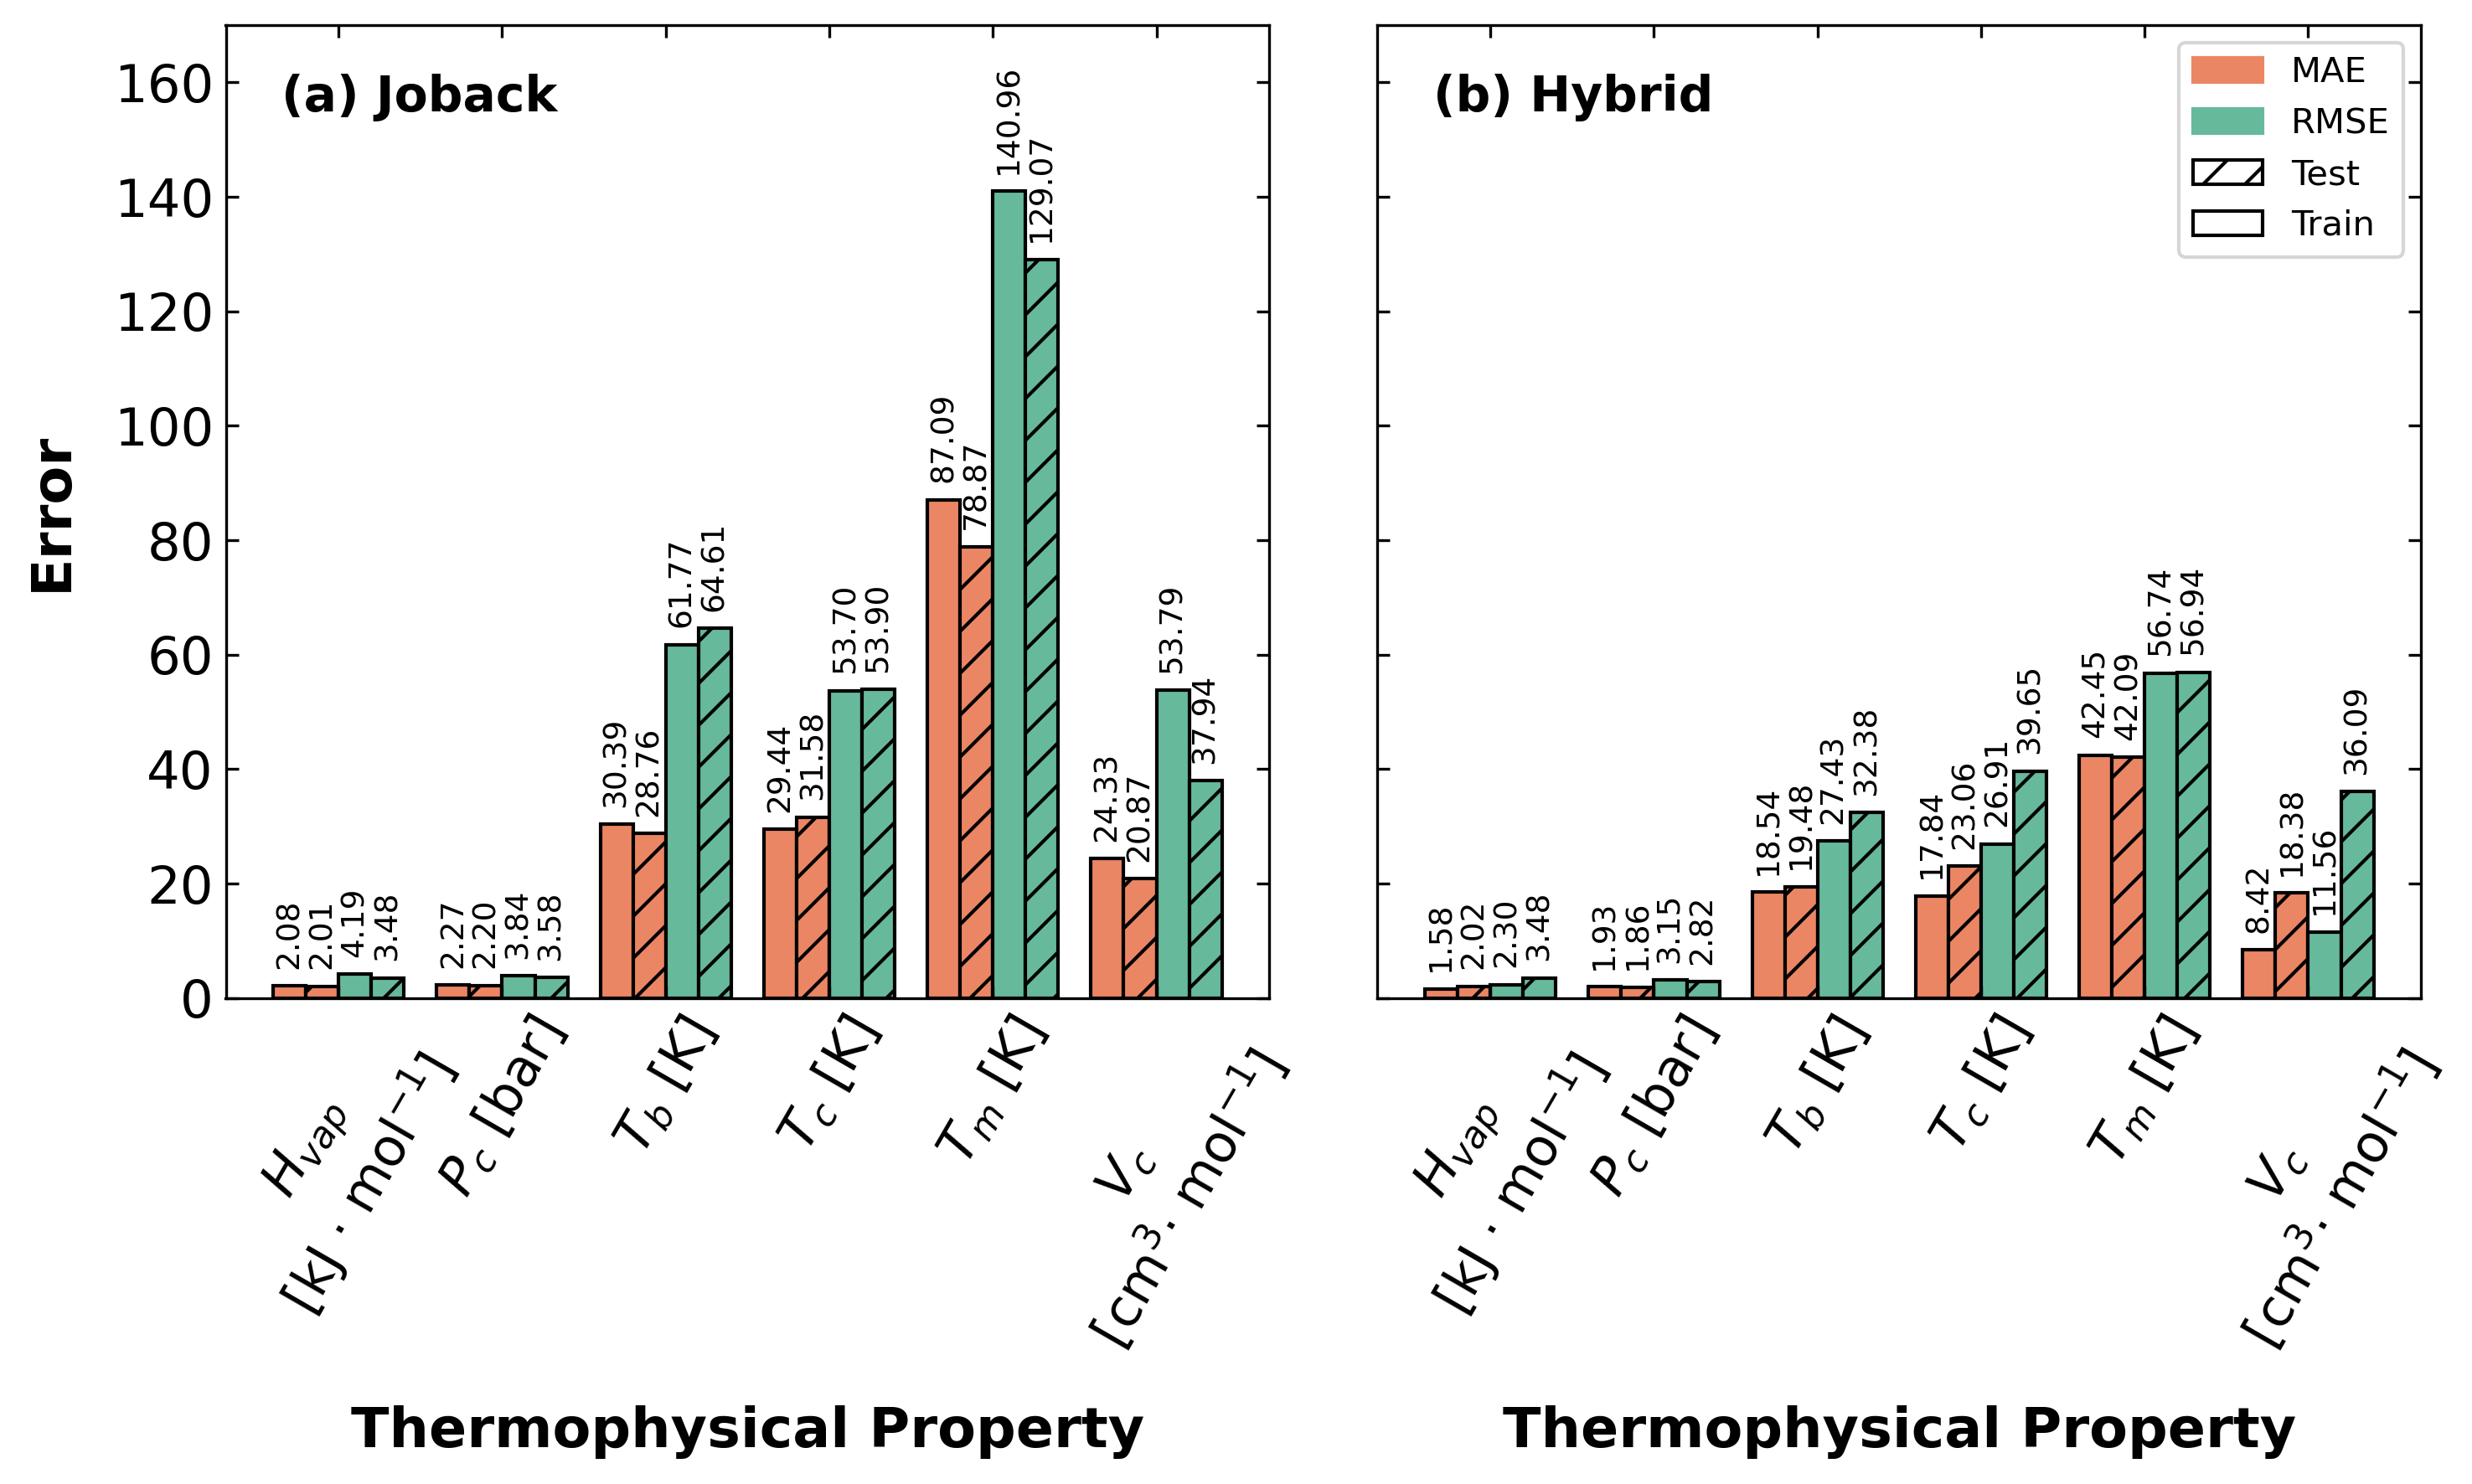
\includegraphics[width=\linewidth]{images/error_bar_chart_shared_yaxis.png}
    \caption{Error vs. thermophysical property of selected GP models for (a) JR and (b) GC-GP models. Salmon (green) represents MAE (RMSE). Solid colors (stripes) represent the training (testing) data.}
    \label{fig: errorbarchart}
\end{figure}

Figure \ref{fig: errorbarchart} shows that GC-GP models significantly reduced the error in JR predictions alone for all models. The only exception appears to be that the test error metrics in JR model (Fig. \ref{fig: errorbarchart} (a)) are marginally less than those of the GC-GP model for $\Delta H_{\text{vap}}$. The explanation for this behavior is straightforward: for both $\Delta H_{\text{vap}}$ and $P_c$, the JR model already makes fairly accurate predictions. As such, adding a GP can increase error since there is uncertainty in estimating the additional parameters in the GP. 

Figure \ref{fig: errorbarchart} (b) shows that for all models except $P_c$ and $T_m$, there is more error in the test set than the training set. This trend is intuitive, as one would expect to see slightly more error in out-of-sample predictions. That being said, significantly higher error rates in out-of-sample predictions could be a result of overfitting. Further analysis is needed to make statements for or against this phenomena in this case study.

\kjnote{I know I've made this a recommendation in meetings several times (see minutes), but I'll just say it one more time. These results would be more robust if we re-generated them with different seeds for a large enough sample of seeds (e.g., 100). This ensures that we didn't get lucky when we did stratified sampling. Ideally, we want the bars of the same color in the LHS plot to be even before we interpret those on the RHS. This bar chart would then report the empirical mean MAE and RMSE across these samples. This would also allow us to add error bars to the top of each bar, thereby accomplishing the uncertainty quantification objective of this paper. If this is not done, I recommend removing the paragraph above.}

\subsubsection{Model selection provides a framework for building robust GC-GP models}
\adnote{Move these plots to the SI. In the discussion above, we observe a handful of interesting issues with the GCGP models. For example, does the LOWER testing versus training error for Pc go away with the best alternative model?}
\kjnote{Im not married to any of my section headings. Feel free to wordsmith or reshape the narrative as the primary authors see fit.}

\adnote{Below is a note from BA in Overleaf on August 4}
\banote{This subsubsection is not present in the outline for this paper for the results section. Please kindly remove all of this.}

\adnote{What is the key to decipher the model name strings?} \kjnote{False means isotropic, True means anisotropic. The main text only looks at isotropic, the si text has anisotropic}

\adnote{Which bar corresponds to the "baseline" GCGP model used throughout the paper?} \kjnote{Model 4}

In order to assess the best performing GC-GP model architecture for each thermophysical property, the (log) evidence model selection criterion (eq.~\eqref{eq: lml}) was calculated. The interpretation of the (log) evidence is straightforward: for each thermophysical property, the model with the greatest (log) evidence is the best model at balancing the trade off between model bias (i.e., how well the model fits the data) and variance (i.e., model complexity). 

Figure \ref{fig: lmlbarchart} shows the log evidence for each thermophysical property investigated (a)-(f). For five model architectures, five isotropic parameterizations of different kernel functions were assessed. The results for the anisotropic kernels can be found in the SI text \kjtodo{Add  reference}. On average, we found that anisotopic parameterizations of the kernel functions did not significantly impact results. As such, the discussion in the main text focuses solely on isotropic kernels. 

Figure \ref{fig: lmlbarchart} shows that model two \kjtodo{reference si} is the worst performing model across all thermophysical properties. This result makes sense, as model two is not complex enough to be informative. Furthermore, model two is the only model that uses only one descriptor (molecular weight). Thus, molecular weight alone is not a good enough descriptor to model GC discrepancy. Taken as a whole, these results confirm our decision to include both molecular weight and GC prediction as descriptors.

Figure \ref{fig: lmlbarchart} shows that model five (eq.~\siref{eq: Model_5}) is the best performing model for all cases except the melting temperature. This result is again explained by the structure of model five. Moreover, model five is the only model that includes a non-stationary mean function. As such, model five is the most flexible and informative model for 5/6 thermophysical properties considered.

\kjnote{I'm not sure how to defend why model four was chosen over model five to generate the results in the main text. I'm also not sure how to explain why the RQ kernel was chosen since the Matern 3/2 kernel was the best performing kernel for 3/6 cases while the RQ kernel was the best performing in only 2/6 cases. I also cannot defend why the Matern 1/2 kernel was not considered for boiling temperature since I did not make this decision. I also cant support the claim that kernel choice doesn't matter, since the results show they are different, if only sometimes marginally.}

\begin{figure}
     \centering
     \begin{subfigure}[b]{0.75\textwidth}
         \centering
         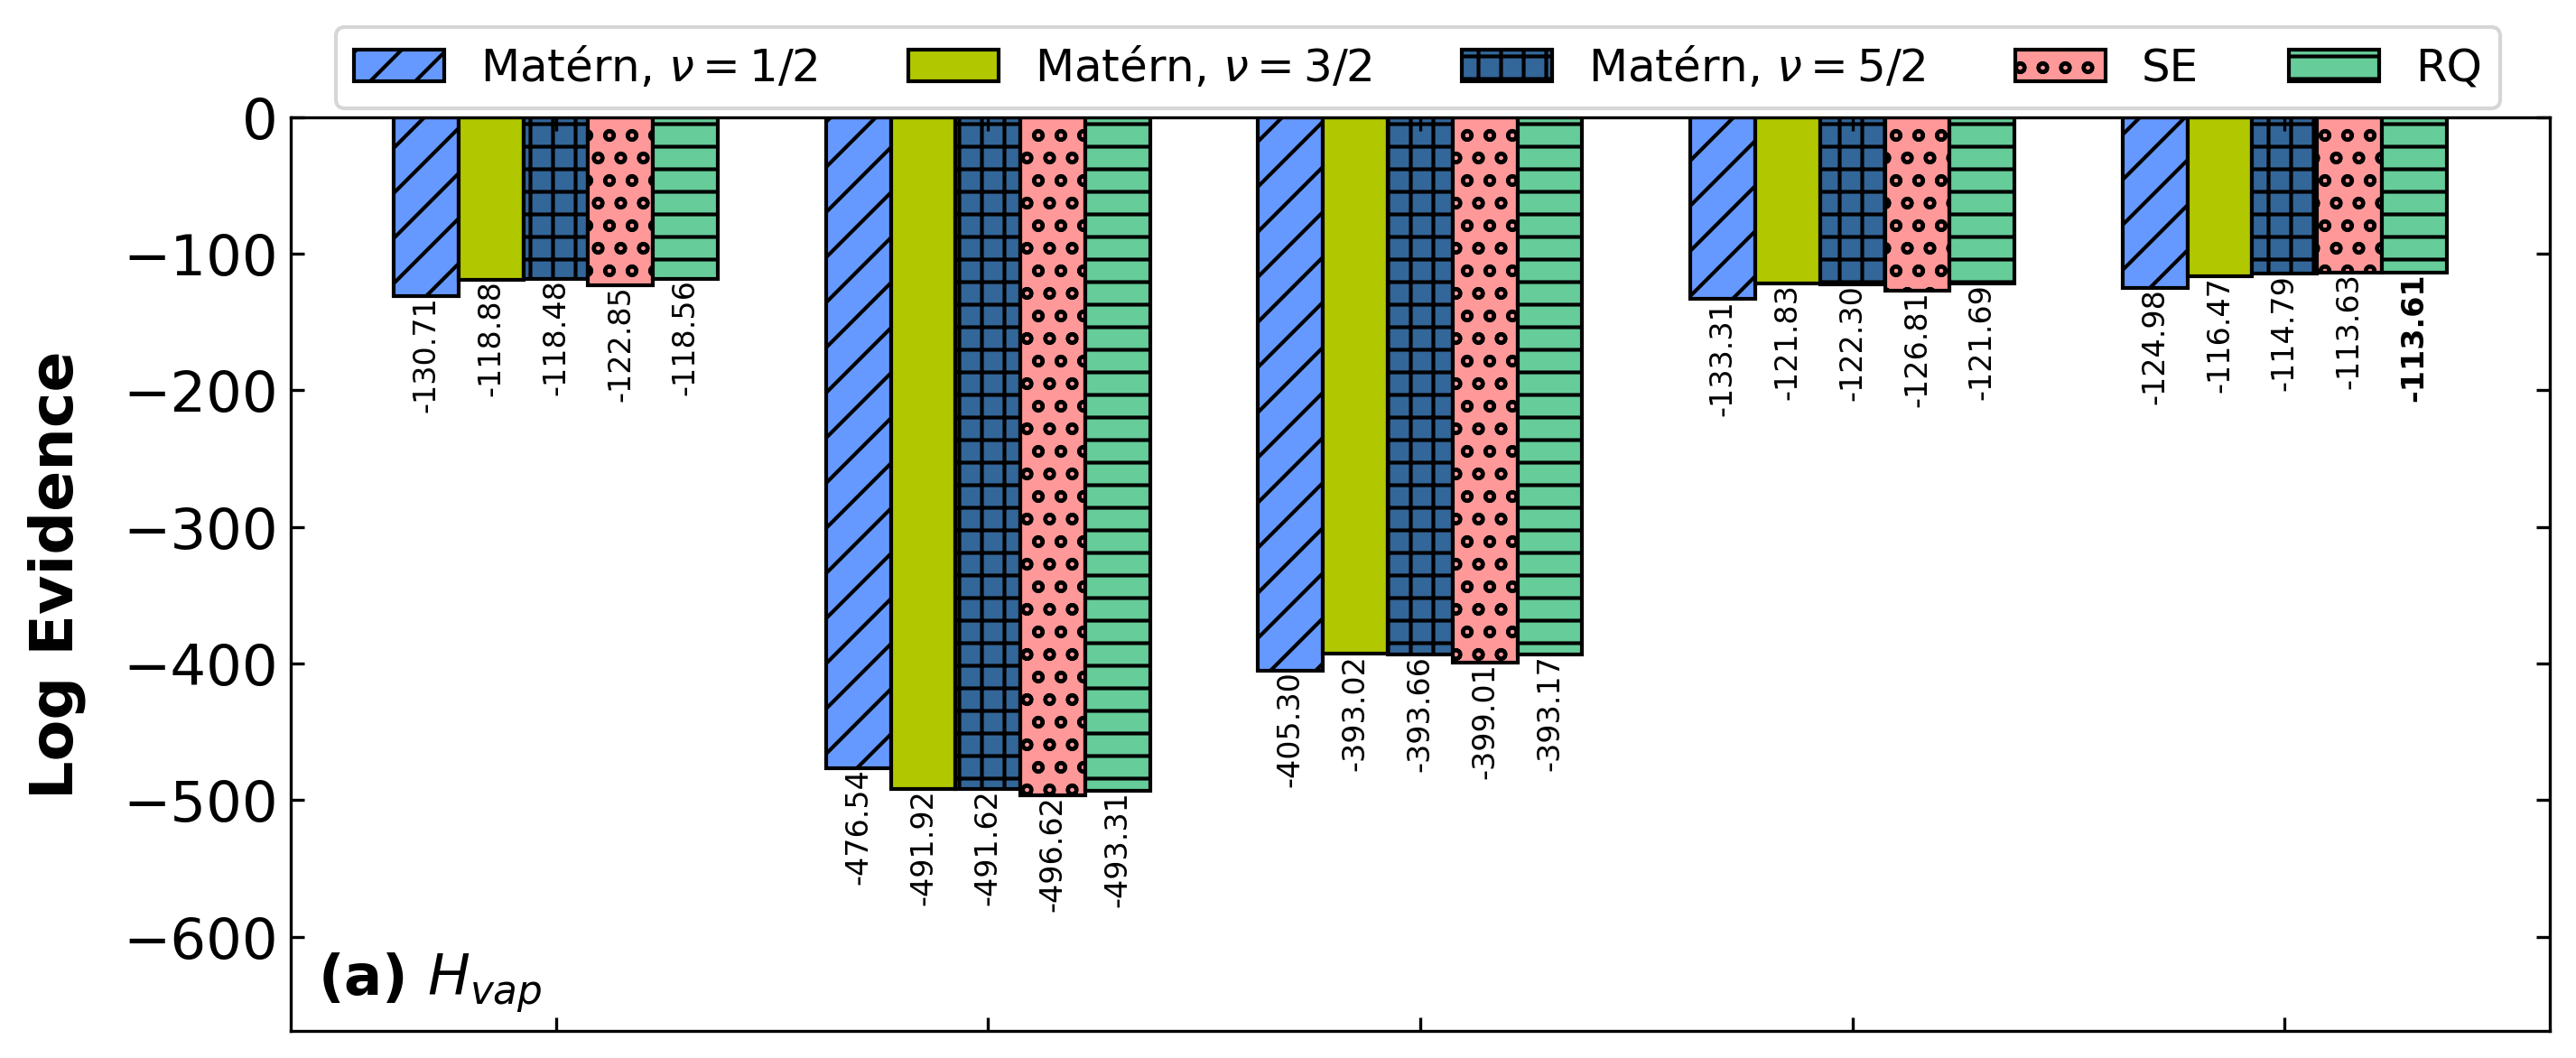
\includegraphics[width=\textwidth]{images/lml_bar_chart_Hvap.png}
     \end{subfigure}
     \hfill
     \begin{subfigure}[b]{0.75\textwidth}
         \centering
         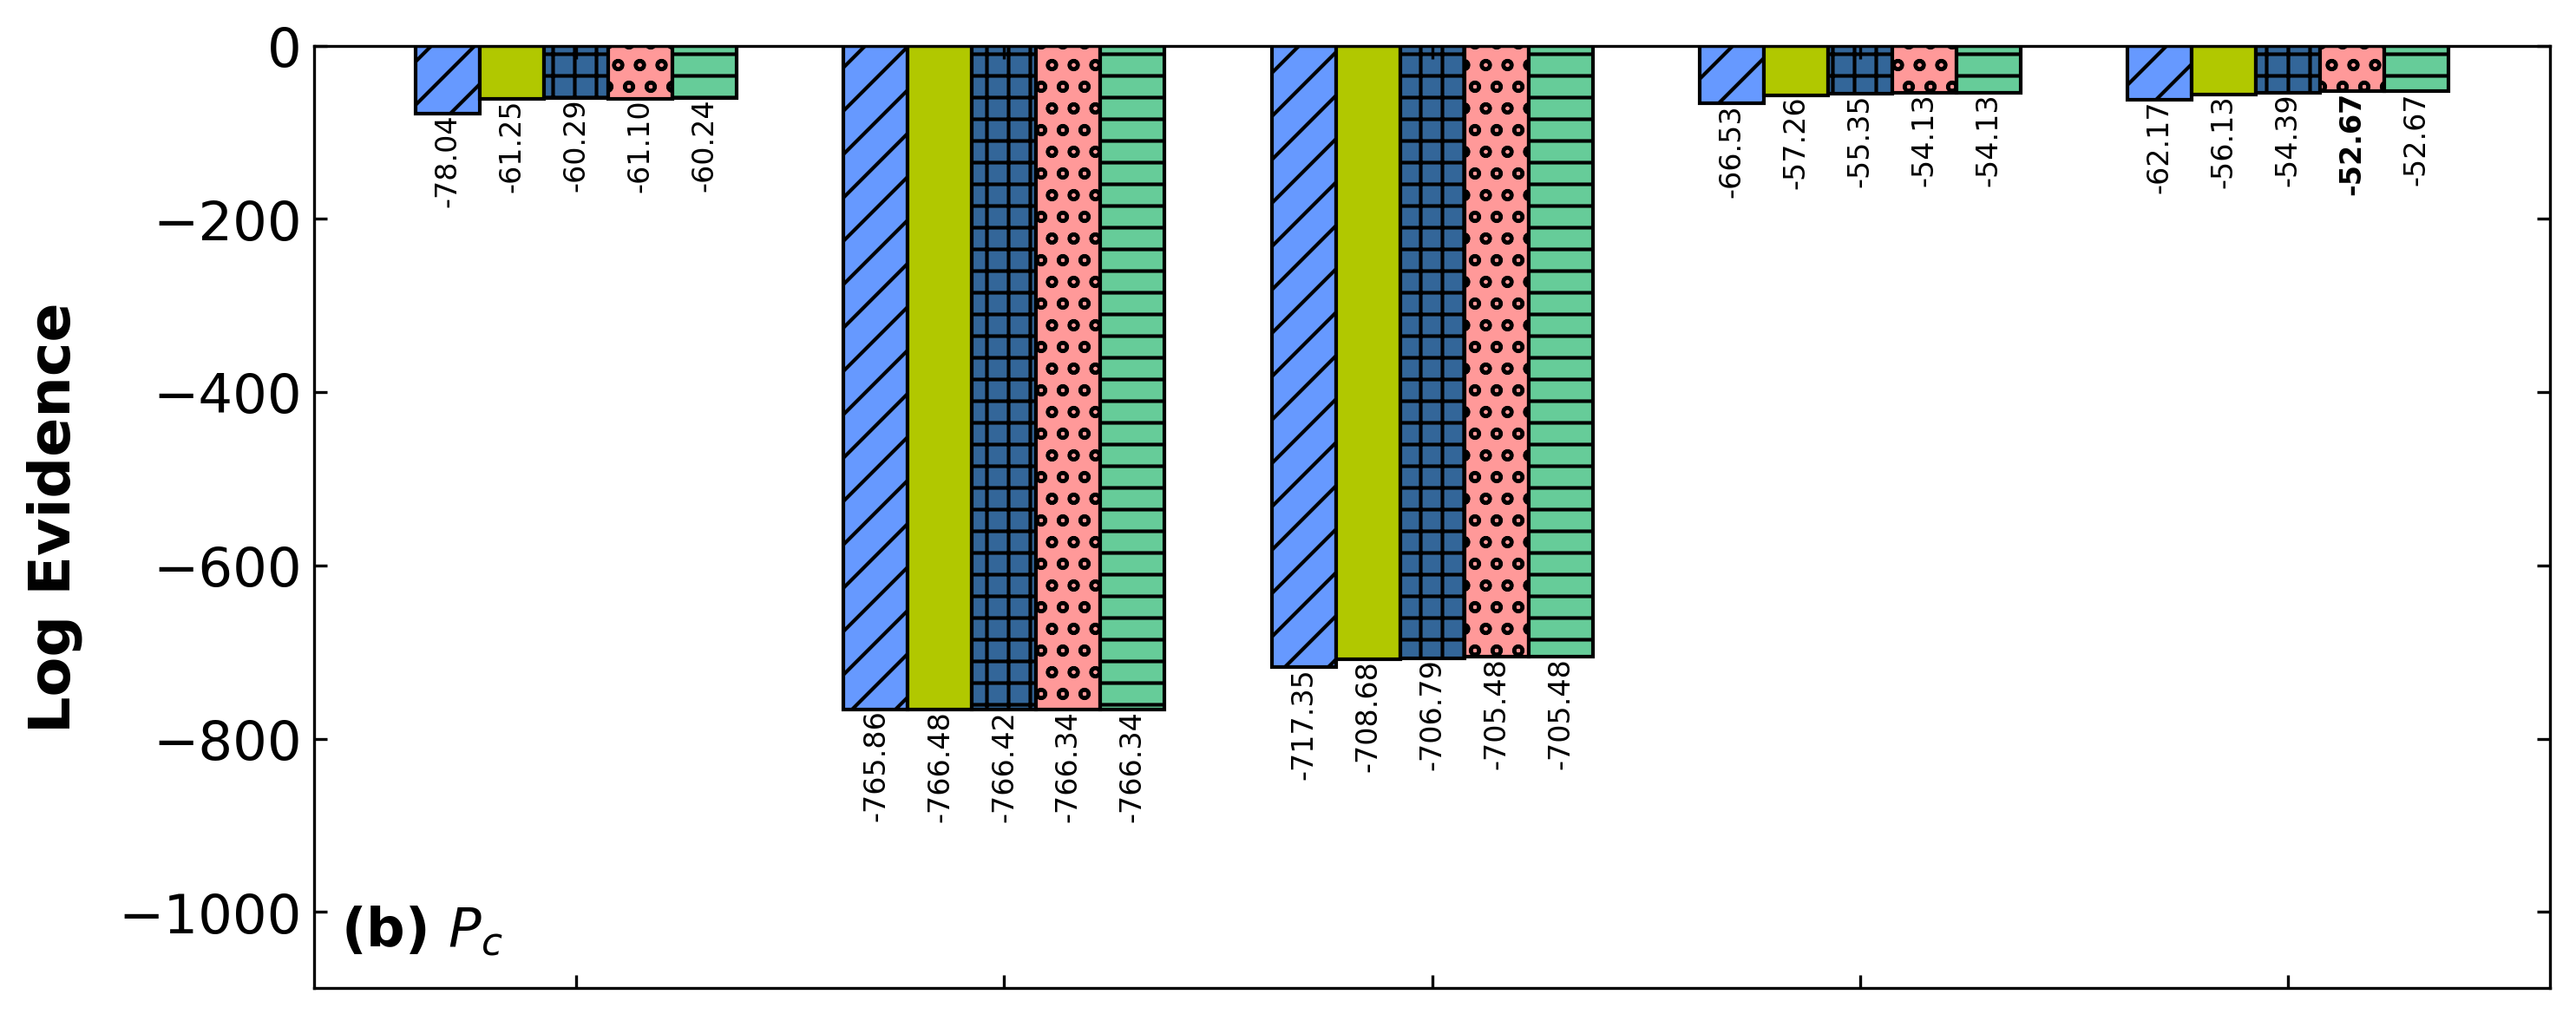
\includegraphics[width=\textwidth]{images/lml_bar_chart_Pc.png}
     \end{subfigure}
     \hfill
     \begin{subfigure}[b]{0.75\textwidth}
         \centering
         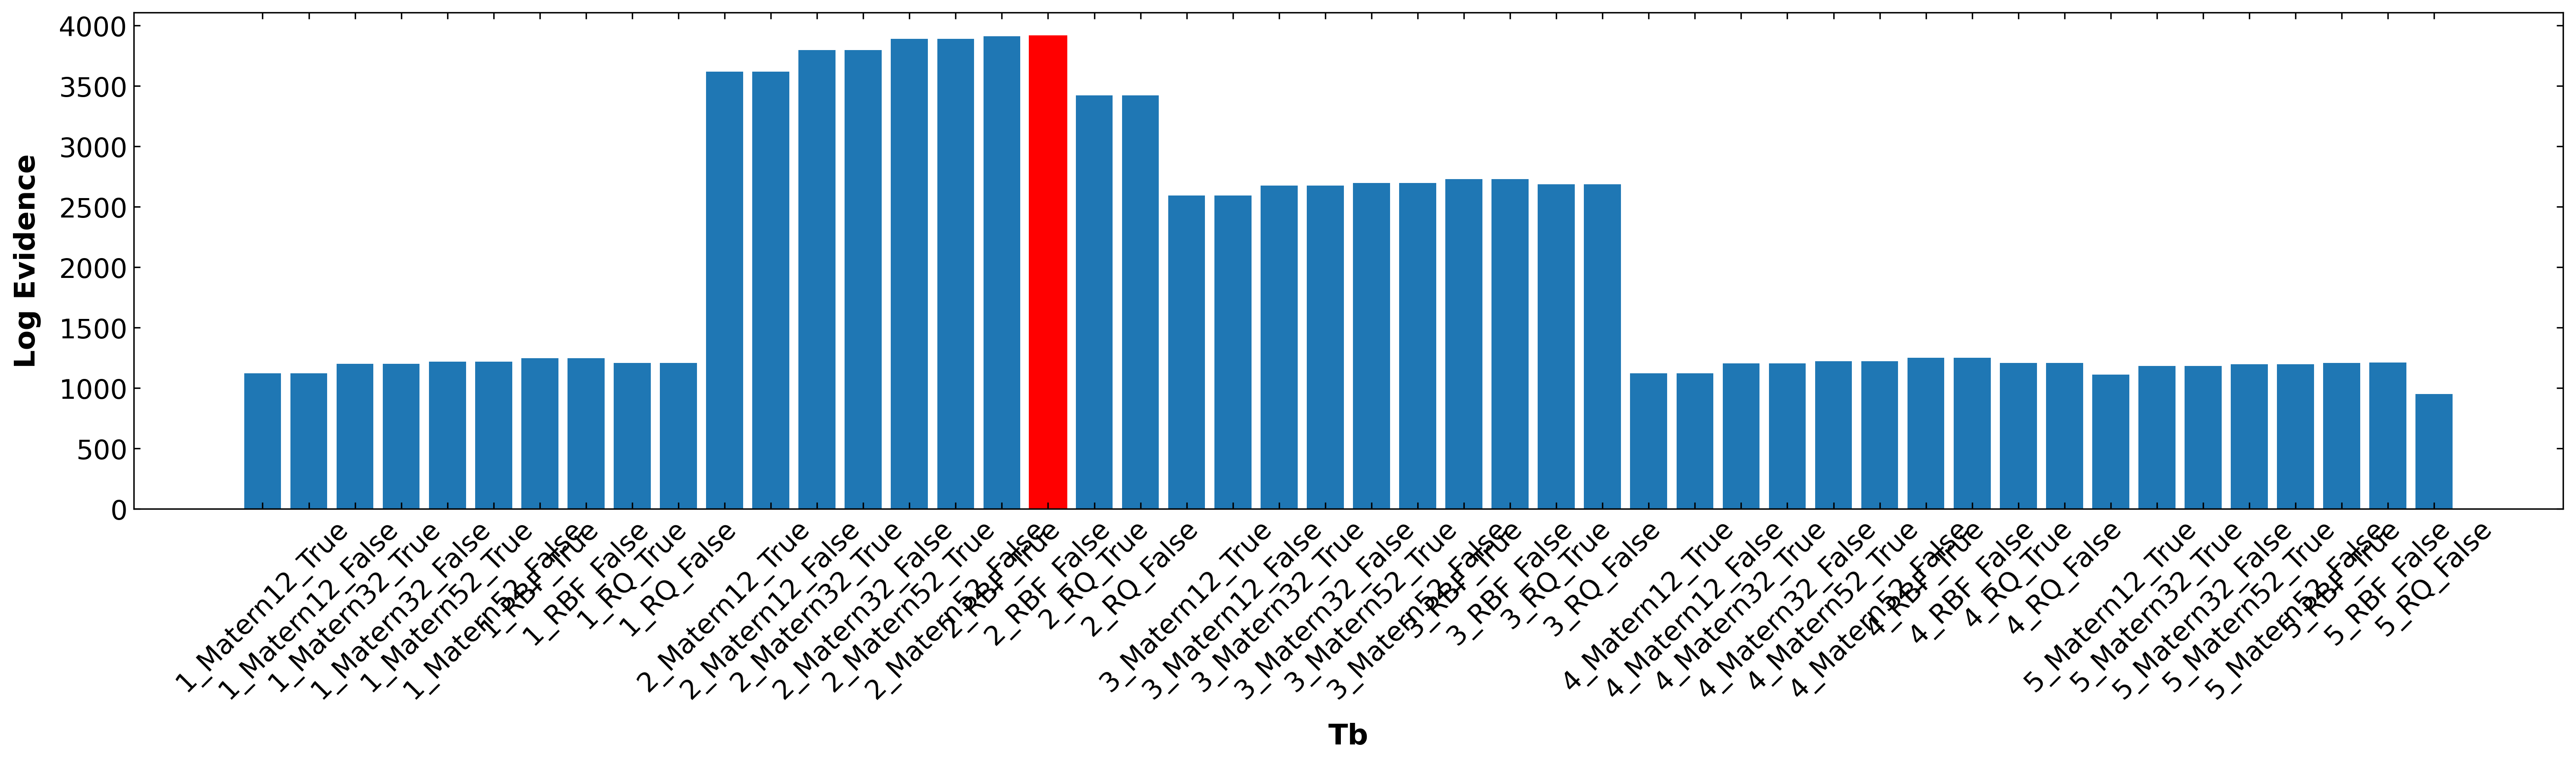
\includegraphics[width=\textwidth]{images/lml_bar_chart_Tb.png}
     \end{subfigure}
     \hfill
     \begin{subfigure}[b]{0.75\textwidth}
         \centering
         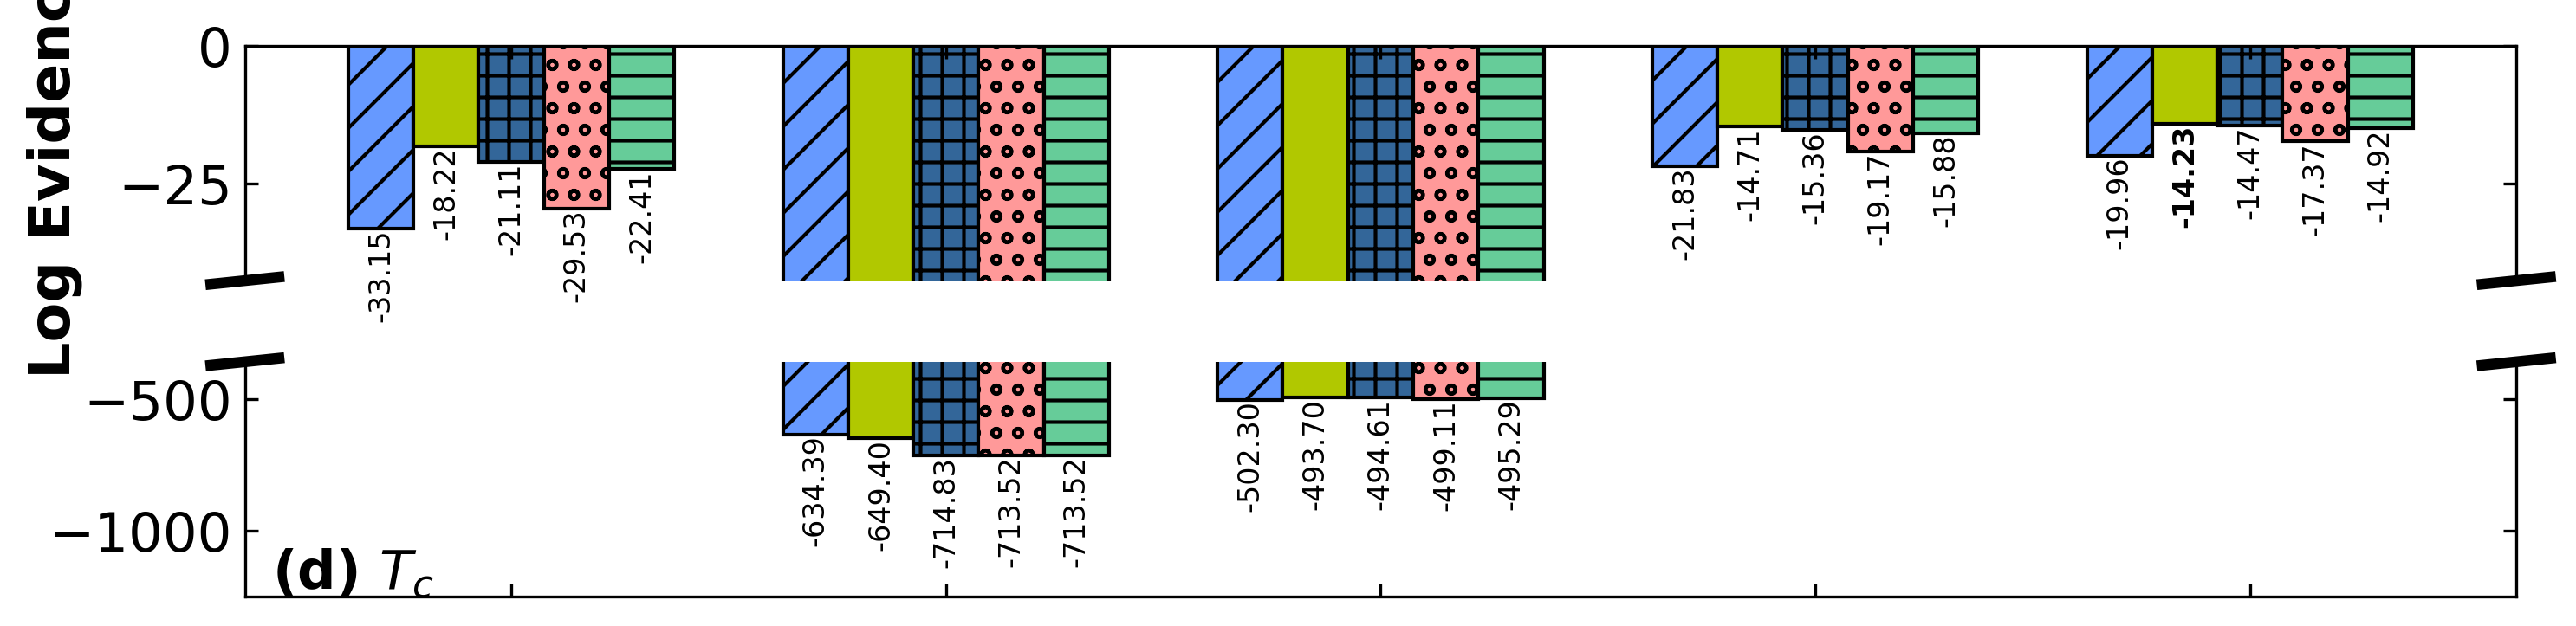
\includegraphics[width=\textwidth]{images/lml_bar_chart_Tc.png}
     \end{subfigure}
     \hfill
     \begin{subfigure}[b]{0.75\textwidth}
         \centering
         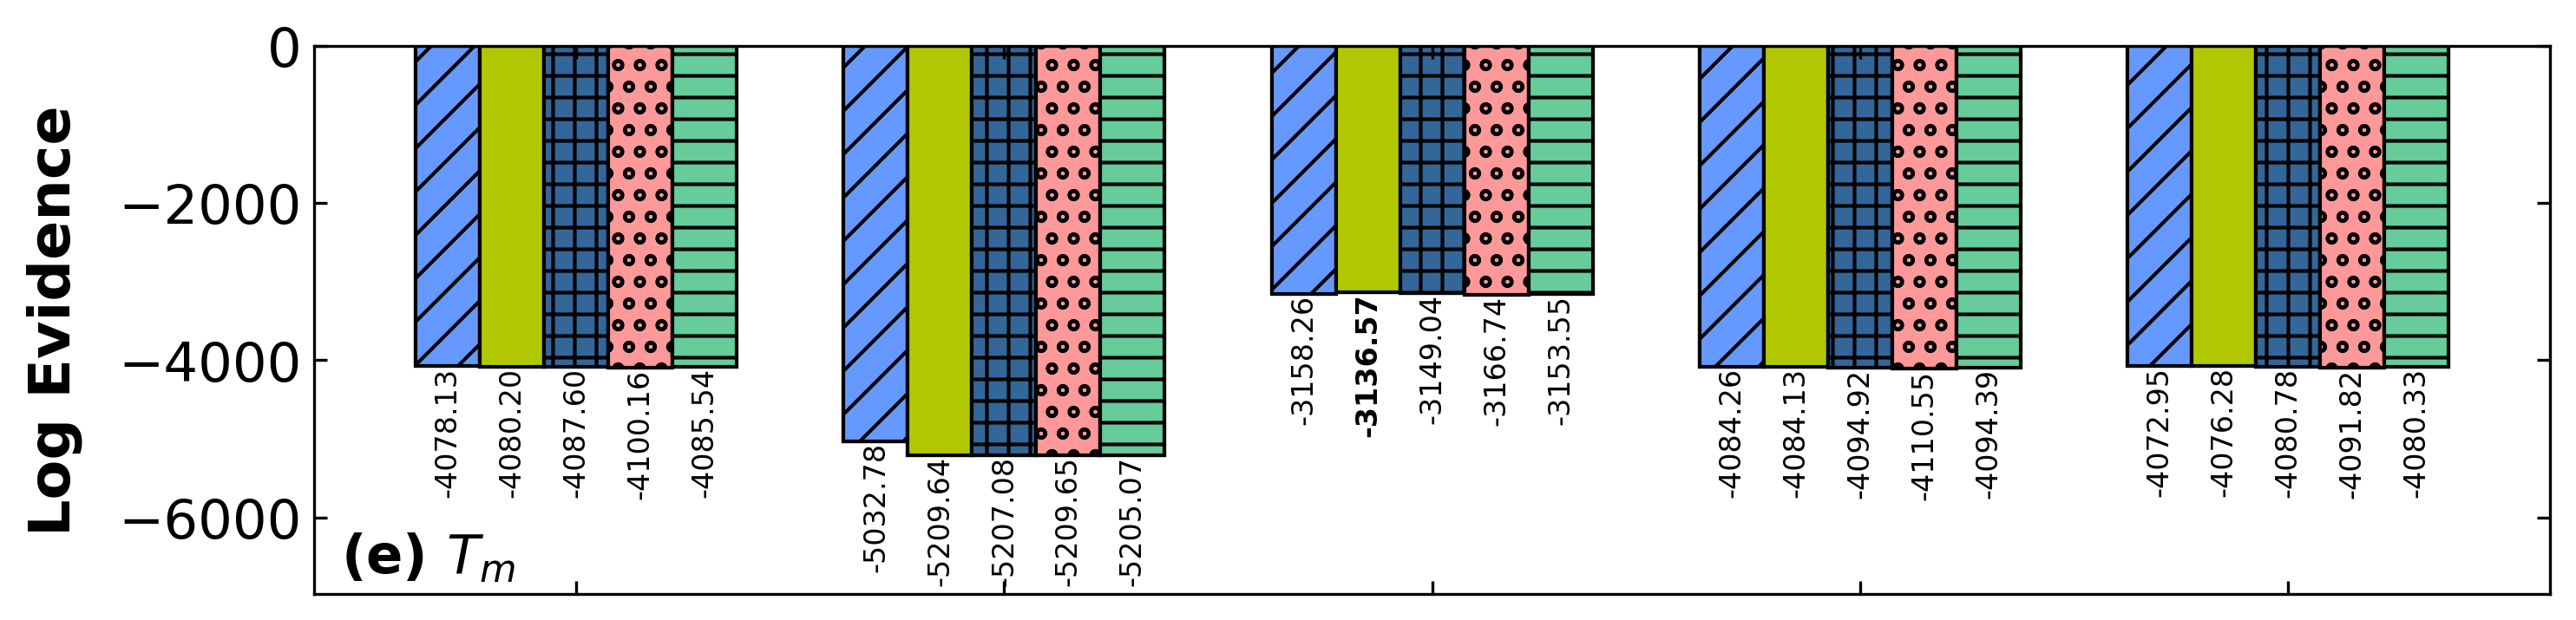
\includegraphics[width=\textwidth]{images/lml_bar_chart_Tm.png}
     \end{subfigure}
     \hfill
     \begin{subfigure}[b]{0.75\textwidth}
         \centering
         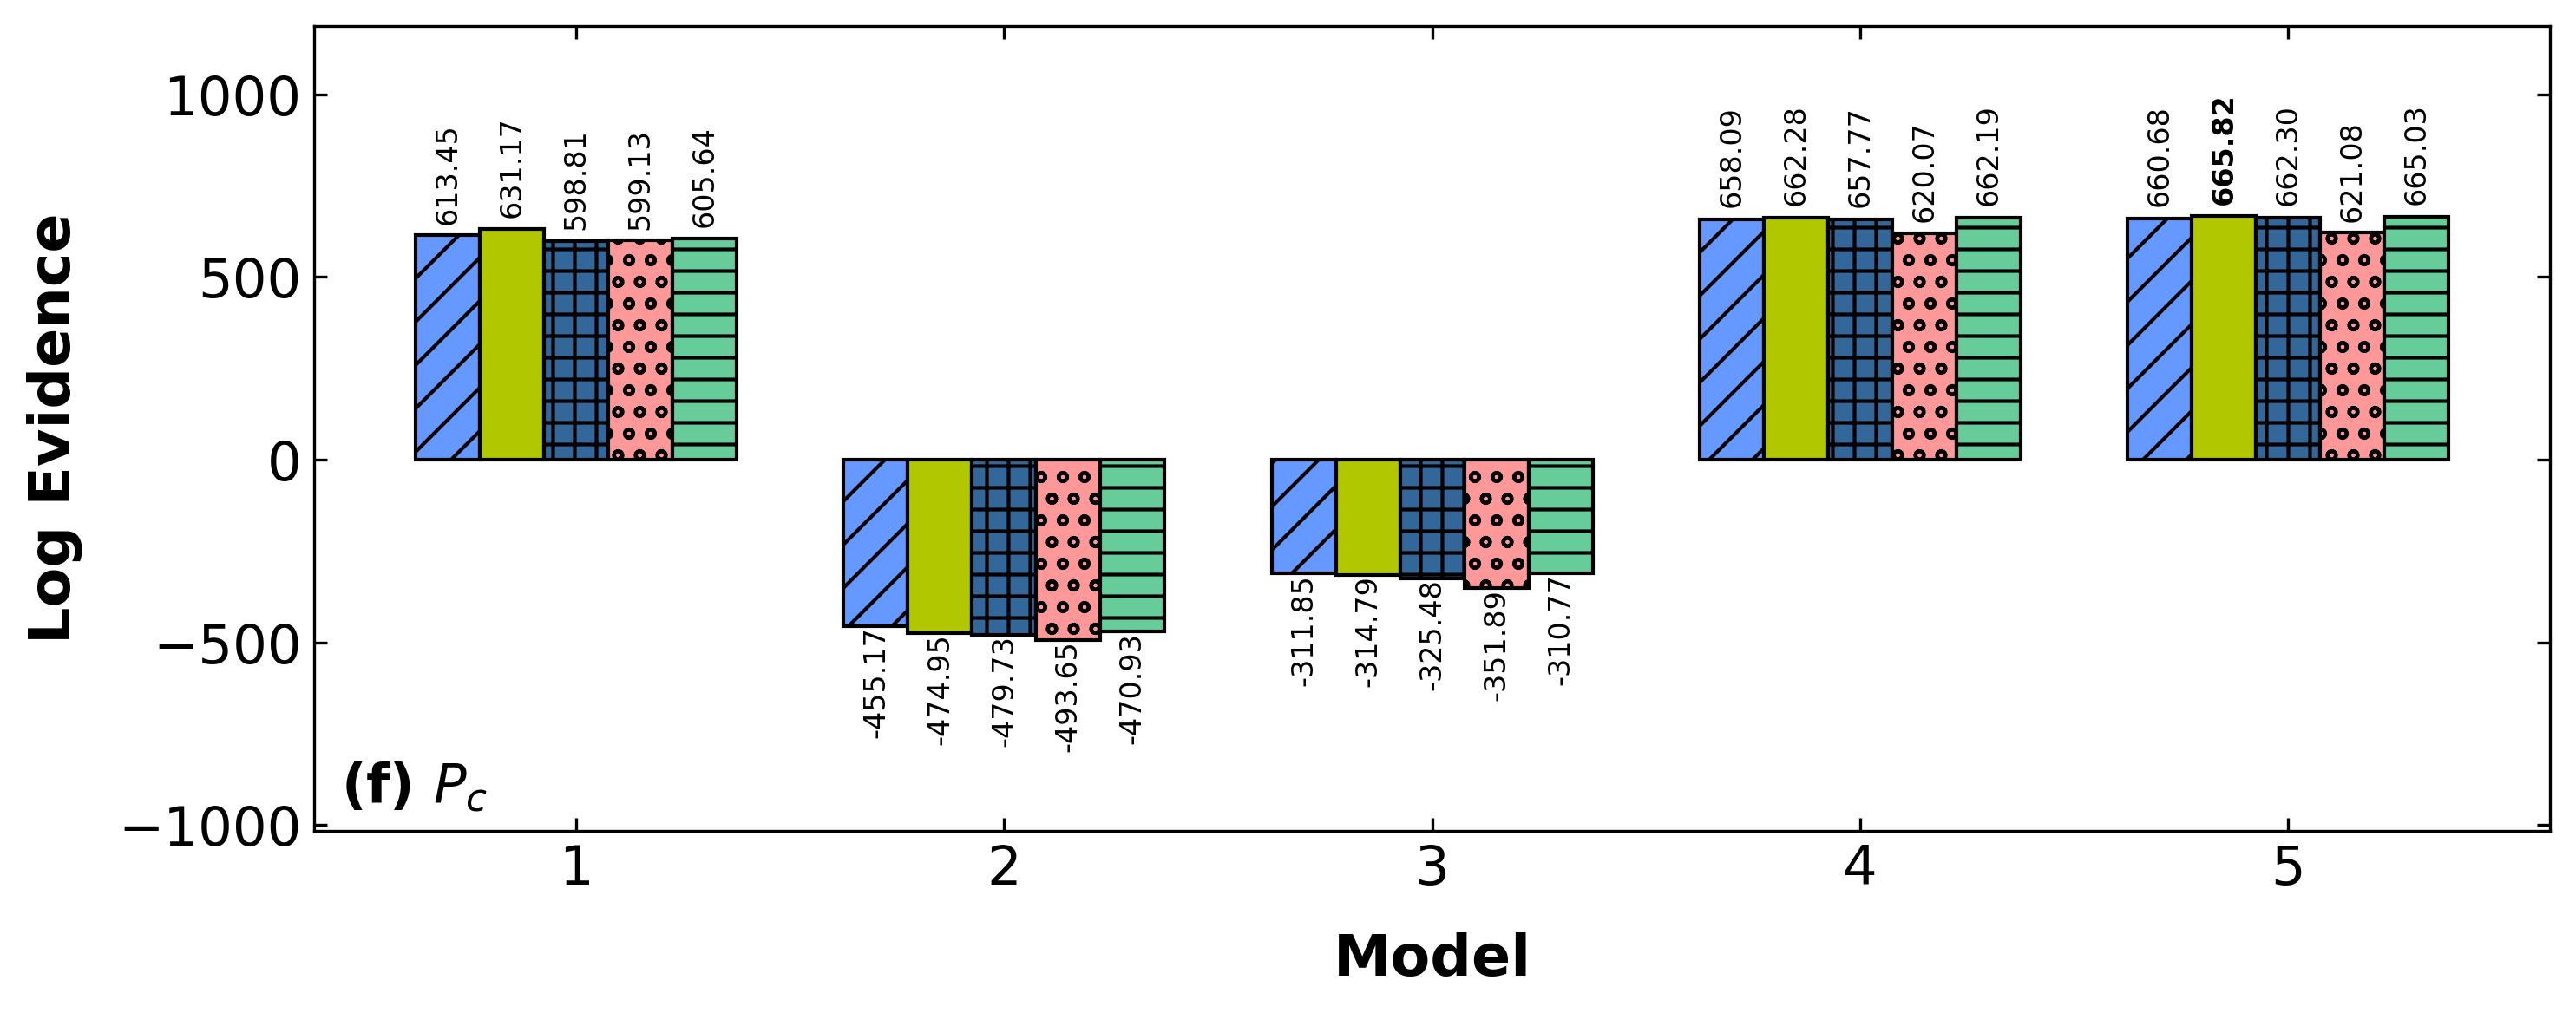
\includegraphics[width=\textwidth]{images/lml_bar_chart_Vc.png}
     \end{subfigure}
     \caption{Log evidence (eq.~\eqref{eq: lml}) vs. model architecture 1-5 (eqs. \siref{eq: Method_1}-\siref{eq: Method_5}) for different isotropic kernels. For each thermophysical property, (a) heat of vaporization, $\Delta H_{\text{vap}}$, (b) critical pressure, $P_c$, (c) boiling temperature, $T_b$, (d) critical temperature, $T_c$, (e) melting temperature, $T_m$, and (f) critical column, $V_c$, the maximum log evidence value is bolded. The blue diagonal striped bars, green solid bars, and navy grid pattern bars represent the Mat\'ern kernel (eq.~\eqref{eq: maternkern}) parameterized by $\nu = 1/2, \, 3/2,$ and $5/2$, respectively. Pink spotted and mint horizontal striped bars represent the squared exponential (eq.~\eqref{eq: sekernel}) and rational quadratic (eq.~\eqref{eq: rationalquadkernel}) kernels, respectively. For boiling temperature (c), the Mat\'ern 1/2 kernel was not tested.
     \alltodo{please explain why or provide this result}. \\
     \kjnote{if the authors use the broken axes when models 6 is added, the y-axis labels will need to be centered manually}
     \kjtodo{put a similar figure for anisotropic kernels in the SI}}
     \label{fig: lmlbarchart}
\end{figure}
\FloatBarrier

\subsection{GCGP approach is robust across kernel and model structure choices} \label{sec:kern_sweep}

\adnote{Shorten this down to one paragraph. Does the sensitivity analysis of kernel and model structure choices fix some of the oddities noted earlier? What is the main take away message from this section?}

\begin{table}[htbp]
    \centering
    \begin{tabular}{l>{\centering\arraybackslash}p{1.0cm}>{\centering\arraybackslash}p{0.9cm}>{\centering\arraybackslash}p{0.9cm}>{\centering\arraybackslash}p{1.8cm}>{\centering\arraybackslash}p{0.9cm}>{\centering\arraybackslash}p{0.9cm}>{\centering\arraybackslash}p{1.8cm}>{\centering\arraybackslash}p{0.9cm}>{\centering\arraybackslash}p{0.9cm}>{\centering\arraybackslash}p{1.8cm}}
          &&  \multicolumn{3}{c}{\textbf{Model 1}}&  \multicolumn{3}{c}{\textbf{Model 4}}&  \multicolumn{3}{c}{\textbf{Model 5}}\\
  && Test $R^2$& Train $R^2$& LML& Test $R^2$& Train $R^2$& LML& Test $R^2$& Train $R^2$&LML
\\
  \textbf{$T_b$} &Mt12& 0.895& 0.953& -1122.618& 0.881& 0.953& -1123.100& 0.886& 0.957&-1113.437
\\
  &Mt32& 0.896& 0.903& -1202.503& 0.839& 0.902& -1205.319& 0.882& 0.907&-1184.224
\\
  &Mt52& 0.893& 0.897& -1219.688& 0.808& 0.897& -1223.621& 0.882& 0.901&-1197.708
\\
  &RBF& 0.888& 0.891& -1247.278& 0.783& 0.890& -1252.692& 0.880& 0.897&-1211.300
\\
  &RQ& 0.892& 0.907& -1209.425& 0.859& 0.908& -1207.450& 0.892& 0.991&-950.841
\\
  &RQ(2)& 0.892& 0.907& -1209.425& 0.860& 0.908& -1207.412& 0.893& 0.991&-949.739
\vspace{0.23cm} \\
  \textbf{$\Delta H_{vap}$} &Mt12& 0.823& 0.956& -130.712& 0.824& 0.956& -133.307& 0.824& 0.952&-124.982
\\
  &Mt32& 0.828& 0.925& -118.881& 0.827& 0.925& -121.832& 0.827& 0.927&-116.466
\\
  &Mt52& 0.830& 0.923& -118.483& 0.828& 0.922& -122.304& 0.829& 0.925&-114.786
\\
  &RBF& 0.821& 0.914& -122.182& 0.821& 0.913& -125.880& 0.832& 0.925&-113.634
\\
  &RQ& 0.832& 0.924& -118.556& 0.830& 0.924& -121.687& 0.832& 0.925&-113.605
\\
  &RQ(2)& 0.847& 0.919& -102.830& 0.850& 0.919& -105.169& 0.851& 0.919&-99.402  
\vspace{0.23cm} \\
  \textbf{$P_c$} &Mt12& 0.941& 0.957& -78.037& 0.942& 0.950& -66.534& 0.942& 0.949&-62.170
\\
  &Mt32& 0.945& 0.938& -61.249& 0.945& 0.938& -57.264& 0.945& 0.938&-56.134
\\
  &Mt52& 0.945& 0.937& -60.290& 0.945& 0.937& -55.354& 0.945& 0.937&-54.387
\\
  &RBF& 0.945& 0.937& -61.097& 0.945& 0.937& -54.133& 0.946& 0.937&-52.668
\\
  &RQ& 0.945& 0.937& -60.240& 0.945& 0.937& -54.133& 0.946& 0.937&-52.669
\\
          &RQ(2)&  0.944&  0.937&  -58.714&  0.945&  0.937&  -54.133&  0.946&  0.937& -52.664     
\vspace{0.23cm} \\
          \textbf{$V_c$} &Mt12&  0.982&  0.999&  613.446&  0.982&  0.999&  658.085&  0.982&  0.999& 660.683
\\
          &Mt32&  0.972&  0.998&  631.173&  0.976&  0.998&  662.275&  0.976&  0.999& 665.821
\\
          &Mt52&  0.981&  0.996&  606.056&  0.974&  0.998&  657.775&  0.975&  0.998& 662.298
\\
  &RBF& 0.984& 0.995& 599.129& 0.982& 0.996& 620.065& 0.982& 0.996&621.083
\\
  &RQ& 0.982& 0.996& 605.638& 0.978& 0.998& 662.185& 0.979& 0.998&665.027
\\
  &RQ(2)& 0.981& 0.996& 605.956& 0.981& 0.998& 664.668& 0.981& 0.998&667.604
\vspace{0.23cm} \\
  \textbf{$T_c$} &Mt12& 0.908& 0.972& -33.151& 0.907& 0.967& -21.828& 0.907& 0.966&-19.964
\\
  &Mt32& 0.897& 0.951& -18.218& 0.898& 0.952& -14.714& 0.898& 0.952&-14.226
\\
  &Mt52& 0.896& 0.950& -21.114& 0.896& 0.951& -15.356& 0.896& 0.951&-14.470
\\
  &RBF& 0.901& 0.942& -28.508& 0.898& 0.950& -19.174& 0.897& 0.951&-17.372
\\
  &RQ& 0.895& 0.951& -22.412& 0.895& 0.951& -15.877& 0.896& 0.951&-14.920
\\
  &RQ(2)& 0.897& 0.951& -21.634& 0.896& 0.951& -15.759& 0.896& 0.951&-14.736 
\vspace{0.23cm} \\
  \textbf{$T_m$} &Mt12& 0.711& 0.731& -4078.129& 0.710& 0.733& -4084.262& 0.712& 0.729&-4072.946
\\ 
  &Mt32& 0.710& 0.711& -4080.198& 0.709& 0.709& -4084.134& 0.711& 0.712&-4076.282
\\
          &Mt52&  0.709&  0.709&  -4087.603&  0.706&  0.706&  -4094.918&  0.711&  0.711& -4080.782
\\
          &RBF&  0.707&  0.705&  -4100.160&  0.701&  0.703&  -4110.552&  0.710&  0.710& -4091.815
\\
          &RQ&  0.711&  0.711&  -4085.540&  0.707&  0.710&  -4094.385&  0.711&  0.711& -4080.326
\\
          &RQ(2)&  0.711&  0.711&  -4085.038&  0.707&  0.709&  -4093.798&  0.711&  0.711& -4080.029
    \end{tabular}
    \caption{Abridged kernel choice and model structure sweep results.}
    \label{tab:kern_sweep}
\end{table}

In Table \ref{tab:kern_sweep}, Mt12, Mt32, Mt52 mean the Mat\'ern 1/2, Mat\'ern 3/2, and Mat\'ern 5/2 kernels. RQ(2) and RQ mean anisotropic and isotropic rational quadratic kernels respectively. RBF mean the radial basis function kernel. LML means the log-marginal likelihood.
Table \ref{tab:kern_sweep} shows that the GCGP method is robust to kernel choice and model structure. The primary difference between models 1, 4, and 5 is in the choice of mean functions. Model 1 has a zero mean function, model 4 has the JR GC predictions as its mean function, and model 5 has a linear function of MW and JR GC predictions with three additional trainable parameters as its mean function.
We find that model 5, with three additional trainable parameters for its mean function, generally does not give significantly higher $R^2$ values on the testing sets compared to model 1 with a zero mean function and model 4 (the model form used in final implementation). Model form 4 is chosen for the final implementation as using the JR GC predictions as the mean function generally makes more physical sense than using a zero mean function. Furthermore, model 4 has a small number of trainable parameters compared to model 5.
The LML, training, and testing $ R2$ values are also similar across various kernel choices in general. The differences between these metrics are generally too small to determine which kernel choice is the 'best' overall for modeling all properties in this work. Thus, we have chosen to maintain a single generally applicable kernel choice and model structure for the final implementation of the GCGP method in this work.
Furthermore, we see that using automatic relevance determination (anisotropic kernels) does not significantly improve model performance.
In this work, we chose the rational quadratic (RQ) kernel with a single length scale as a kernel that is generally applicable for all properties modeled in this work. The RQ kernel has a shape parameter which makes it flexible for use in modeling a variety of data with different or unclear smoothness trends. In summary, the GCGP method gives generally good performance for all properties irrespective of kernel choice. The choice of model structure may have a bigger impact on performance.  \textcolor{red}{Tables AA - ZZ} in the SI show the complete results of the effects of kernel choice and model structure on predictive performance. Model 2, which uses MW as the only input feature to a  GP that models the discrepancy with the JR GC predictions as the mean function, is seen to consistently have the poorest performance among all the model forms. Model 3, another discrepancy model but with a zero mean function and with MW and JR GC predictions as the two input features to the GP, shows comparable performance to models 1, 4, and 5. In summary, the GCGP method gives generally similar performance irrespective of kernel choice and mean function choice. However, the JR GC predictions must be used as one of the input features (and not just as the mean function as is the case for model 2) to obtain good performance.


\subsection{Extensibility and Opportunities for Future Work}
\adnote{Merge this with next section, "Conclusions and Future Work"}

%Barnabas to provide specific examples
Although this work focuses on six properties and a Joback and Reid group contribution method, the technique for creating models is directly applicable to other properties and other GC methods. 
%A GP model can be built using the same steps as in this work as long as the GC method can provide the property prediction. GC prediction and property data must be rigorously analyzed to determine appropriate features for the model. Their relationships should be analyzed to collect and apply a priori information including well-known physical correlations. With appropriate scaling, a model can then be trained and validated to produce improved accuracy results with uncertainty information.
The GCGP method may be considered a tunable method for improved predictive accuracy. As an example, we observed in this work that the GCGP method gave the least performance in terms of predictive accuracy for $T_m$. This was mainly attributed to the extreme bias in the JR GC predictions of $T_m$ which was used as input to the corrector GP model. A simple way to improve the prediction of $T_m$ using the GCGP approach is to switch to a more accurate but still simple GC method for predicting GC $T_m$. Indeed, such a method already exists \cite{perezponceNewGroupContribution2013}. Alternatively, we can use the same structural unit definition as the JR GC method but design a more accurate GC model functional form and parameterize the more advanced GC model functional form using collected data. This likely more accurate GC model can then be used to obtain input GC predictions in the GCGP method. This later approach is more likely to lead to significant improvement in predictive accuracy for $T_m$. Molecules that cannot have their properties predicted due to the limitations of unavailable parameters in a given GC method can have their properties predicted by switching the GC method to another one that is able to predict their properties. The above recommendations are examples of how the GCGP method may be easily tuned to obtain even better predictive accuracy or extended to other properties and molecule types not considered in this work. 
Furthermore, one opportunity for future contribution will be to extend the GCGP method to predict properties at varying conditions of temperature and possibly pressure. This may be achieved by adding temperature as an input feature to the GP and training against sufficient data to capture the temperature dependence of the target property. There are very likely several other and probably more effective ways to achieve this.
It would be interesting to see what nuances may be encountered and how the GCGP method performs when applied to GC-based thermodynamic models.
Another contribution that would be highly valuable is integrating the GCGP method with CAMD workflows. The improved predictive accuracies and easily accessible uncertainty estimates from the GCGP method could result in significant improvement in the reliability and robustness of CAMD workflows in identifying optimal molecules and processes for a variety of applications.


\section{Conclusions}
We have developed and demonstrated a property prediction method that integrates the strengths of GC-based molecular models for property predictions with GPR for high predictive accuracy with reasonable uncertainty estimates. The GCGP method corrects systematic bias in GC-based property modeling and offers significant improvement in predictive accuracy over the GC-only predictions. The GCGP approach is robust to choice of GP kernels and model structure provided the GC predictions are used as one of the input features to the GP. Furthermore, the GCGP method has a high potential to be tunable to give even better predictive accuracies and can be conveniently extended to other properties, GC models, and molecule types not considered in this work. 
The GCGP method developed in this work thus offers a fast, simple, reliable, generalizable, and tunable property prediction method that gives predicted uncertainties for the property predictions. The GCGP method therefore offers a key tool for reliable property prediction for materials screening in material discovery tasks. 
Several opportunities exist for future contributions, such as integrating the GCGP method into CAMD workflows, applying the GCGP method to GC-based thermodynamic models and engineering correlations in general, and extending the method for predicting temperature and pressure-dependent properties as well as mixture properties.

\adnote{More future work paragraph to here. Edit to tighten and remove redundancies.}


\section{Nomenclature}

%%%%%%%%%%%%%%%%%%%%%%%%%%%%%%%%%%%%%%%%%%%%%%%%%%%%%%%%%%%%%%%%%%%%%
%% The "Acknowledgement" section can be given in all manuscript
%% classes.  This should be given within the "acknowledgment"
%% environment, which will make the correct section or running title.
%%%%%%%%%%%%%%%%%%%%%%%%%%%%%%%%%%%%%%%%%%%%%%%%%%%%%%%%%%%%%%%%%%%%%
\begin{acknowledgement}
The authors acknowledge funding from the National Science Foundation (NSF) EFRI DChem: Next-generation Low Global Warming Refrigerants, Award no.~2029354. BA \& KJ acknowledge the Notre Dame Lucy Institute for Data and Society. BA acknowledges the Notre Dame Energy for graduate research fellowships. Computational resources were provided by the Center for Research Computing (CRC) at the University of Notre Dame. MC \& KJ acknowledge support from the Graduate Assistance in Areas of National Need fellowship from the Department of Education via grant number P200A210048, the National Science Foundation via Award numbers CBET-1917474 and EFRI-2029354, and the University of Notre Dame College of Engineering and Graduate School.  

\end{acknowledgement}

%%%%%%%%%%%%%%%%%%%%%%%%%%%%%%%%%%%%%%%%%%%%%%%%%%%%%%%%%%%%%%%%%%%%%
%% The same is true for Supporting Information, which should use the
%% suppinfo environment.
%%%%%%%%%%%%%%%%%%%%%%%%%%%%%%%%%%%%%%%%%%%%%%%%%%%%%%%%%%%%%%%%%%%%%
\begin{suppinfo}
The Supporting Information is available free of charge.

%Calculated properties, sample input scripts, and post-processing codes used in this work are available to the public on the project's \href{https://osf.io/t9265/}{Open Science Framework} and \href{https://github.com/MaginnGroup/Validation-of-HFC-FFs}{GitHub} repository at \\
%https://osf.io/t9265/ and https://github.com/MaginnGroup/Validation-of-HFC-FFs, respectively.
\end{suppinfo}

%%%%%%%%%%%%%%%%%%%%%%%%%%%%%%%%%%%%%%%%%%%%%%%%%%%%%%%%%%%%%%%%%%%%%
%% The appropriate \bibliography command should be placed here.
%% Notice that the class file automatically sets \bibliographystyle
%% and also names the section correctly.
%%%%%%%%%%%%%%%%%%%%%%%%%%%%%%%%%%%%%%%%%%%%%%%%%%%%%%%%%%%%%%%%%%%%%

\bibliography{GCGP_refs}

\end{document}
